%!TEX root = ../thesis.tex

\chapter{Results}
\label{chap:r}

In the previous chapter, I described the theoretical structure of my processing pipeline, giving a detailed account of the algorithms and procedures relevant to each pipeline step. Being the result of a process of iterative refinement and revision, these were partly based, in fact, on my practical experience at implementing them and testing how effective they are at fulfilling their roles. As a result, the final methods and results of this research are interlinked and were thus difficult to separate into two chapters.

In this section, I will not dedicate much attention to the changes introduced during development, as I already addressed this topic in the previous chapter. Instead, I will restrict the discussion to focus only on the relationship between the final version of the code and the outputs it produces. In this chapter, I will only mention the challenges that lead to changes in the system design, where figures are shown that illustrate them well.

In the following sections (\ref{sec:manualpreprocessing}, \ref{sec:results}), I will show the intermediate results of each step of the pipeline visually in figures, as well as describe them in the text. This showcase and description of the results will focus primarily on the effectiveness of the final implementation and system design, and the quality of the results it produces.

The last sections of the chapter (\ref{sec:accuracy}, \ref{sec:r_comparison}) contains a section in which the results of quantifying the quality and accuracy of the output are shown and discussed, followed by a section in which the commercial results and the present academic results are compared, especially in terms of the overall quality of the results they produce.

\section{Manual pre-processing}
\label{sec:manualpreprocessing}

\subsection{Producing the testing datasets}
\label{sub:testingdataproduction}

\begin{figure}
    \centering
    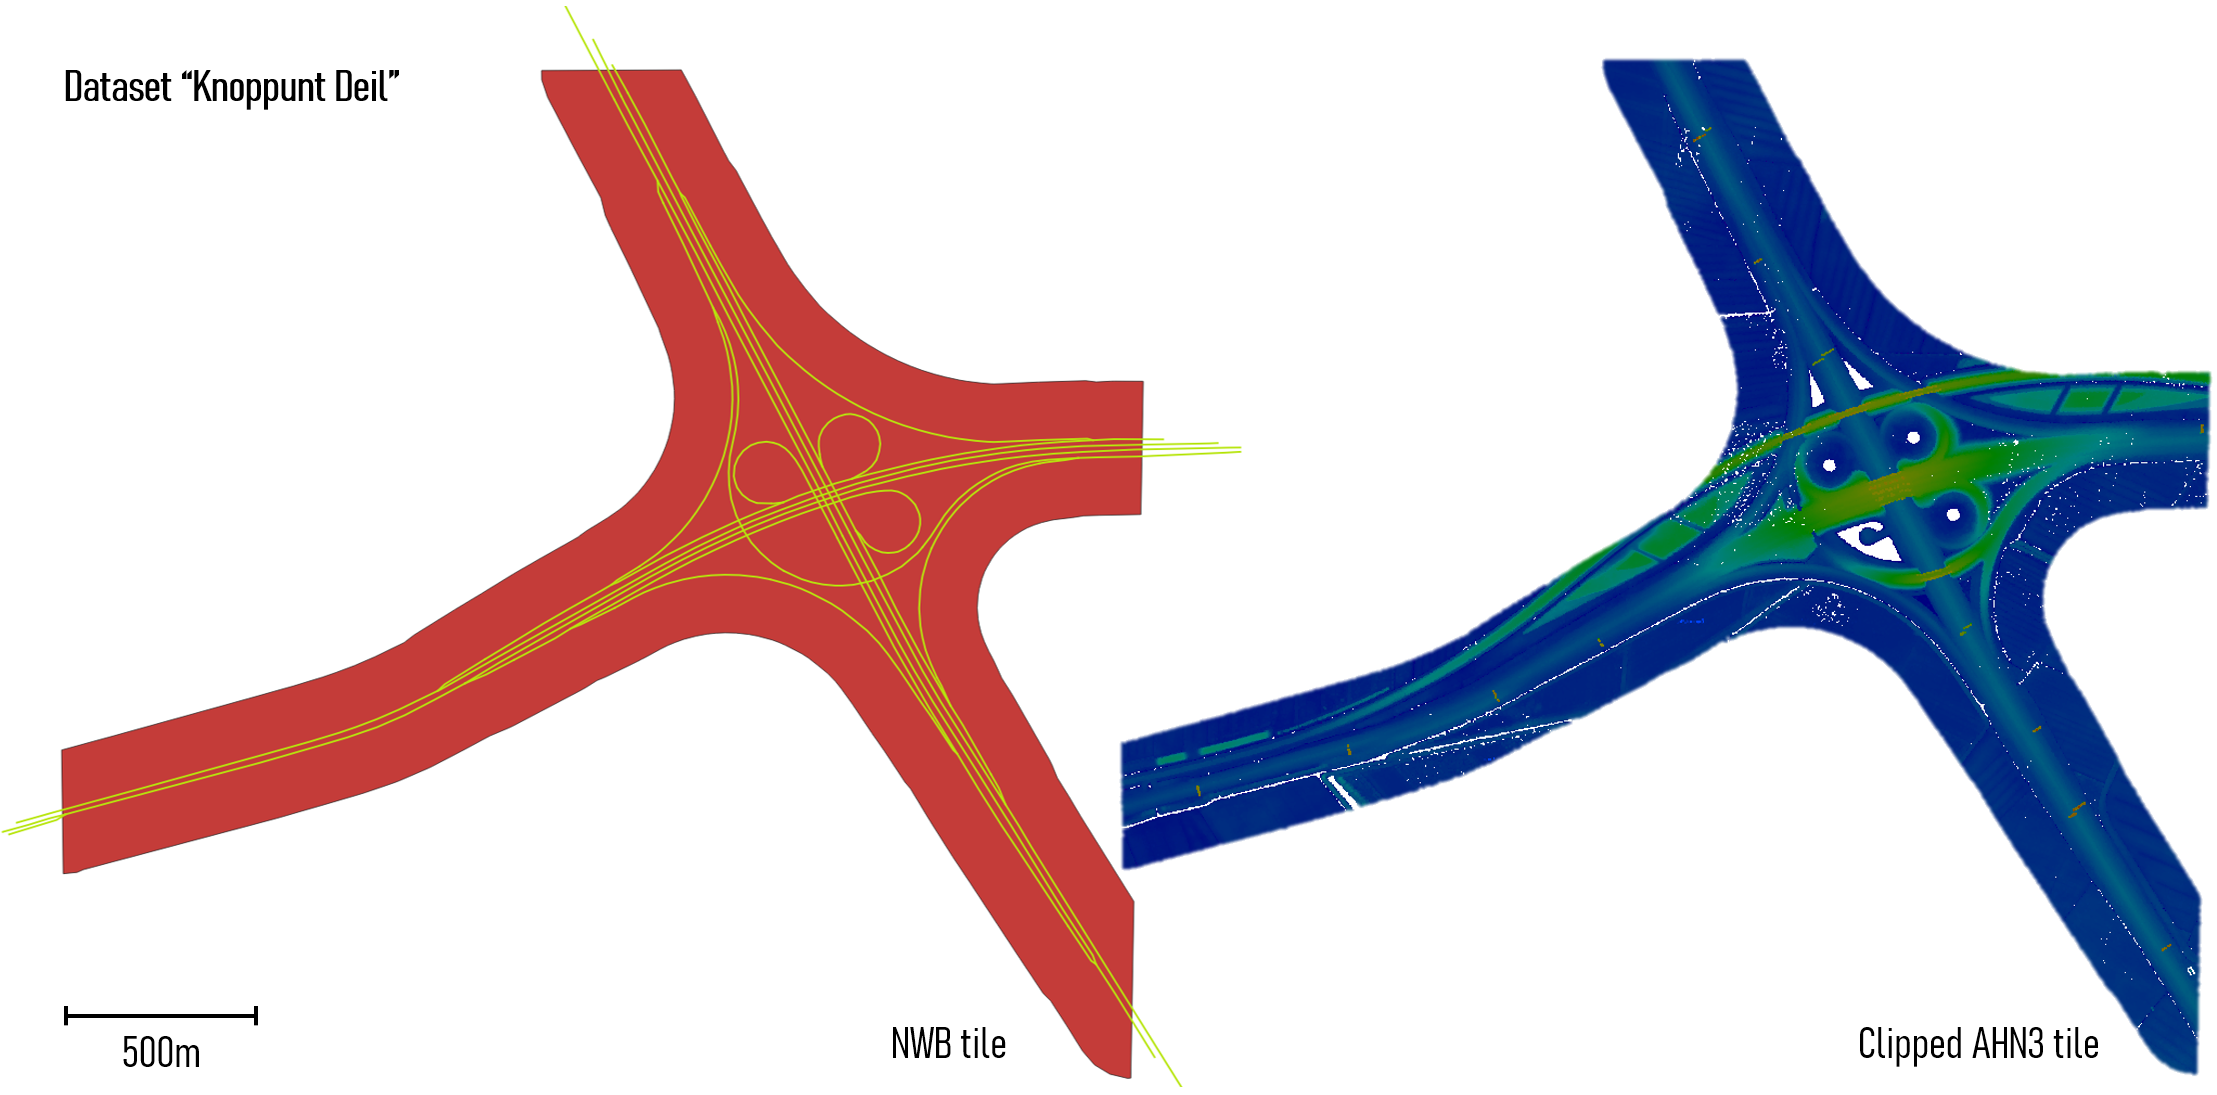
\includegraphics[width=\linewidth]{final_report/figs/manualpreprocessing.png}
    \caption{Visualisations illustrating the results of manual pre-processing.}
    \label{fig:manualpreprocessing}
\end{figure}

Implementing a scaling solution was not part of this project, although all parts of the implementation were designed in a way that a scaling framework could be added to it with a relatively small amount of effort. Among other things, scaling in this project concerns the need to subdivide the input data in a way that the software never runs out of memory while processing it. These subdivisions could be generated, in the simplest case, based on tiling, i.e. overlaying a 2D raster on the extents of the data and examining which cell certain features fall into.

As scaling was not part of this project, the task of creating manageable subsets of the input data was carried out manually. The procedure consisted of cropping the input vector datasets (\ac{nwb}, \ac{dtb}) into tiles showing interesting and representative road layouts, and for each of them, creating an \ac{ahn3} file with those points, which are a set maximum distance from any relevant roads (\ac{r_roads} and \ac{p_roads}) in their respective \ac{nwb} tiles. For vector data processing, I used \textit{QGIS}, and for Lidar processing I used \textit{LASTools}.

I derived the area of interest in which to keep Lidar points by buffering the centrelines in the \ac{nwb} tiles by 150 metres, and passing these geometries on to LASTools to use to \textit{clip} the relevant \ac{ahn3} tiles. \ac{ahn3} itself comes tiled in the official release (on a much larger scale), and I derived each testing dataset from a single \ac{ahn3} tile to keep the manual procedure simple. I also discarded \ac{ahn3} points not classed as ground or bridge points at this stage (2 and 26 respectively), as they are not relevant to our methods.

Visualisations are shown in Figure \ref{fig:manualpreprocessing} in which an \ac{nwb} tile and the Lidar clipping polygon (on the left) is shown alongside the clipped point cloud tile (on the right). The clipping polygon was manually edited to have sharp, linear boundaries and \ac{nwb} \textit{wegvakken} (yellow lines) intersecting its interior (red areas) were included in the testing dataset. The resulting occasional overshoots of \ac{nwb} centrelines (relative to \ac{ahn3}) allowed me to test how well the procedure performs in areas where \ac{ahn3} is completely unavailable for a short distance, but where \ac{dtb} coverage is present - hence, I kept them. They also caused unforeseen issues in the accuracy assessment, which I will discuss in Section \ref{sub:accuracytabulated}. On the right, the point cloud is shown in its original density, not a derived \ac{dtm}. Darker areas represent lower elevations, the total elevation range shown in the image is about ten metres.

I created 11 testing datasets in total, each with its own cropped \ac{nwb}, \ac{dtb} and \ac{ahn3} files, which are described in the next section. The dataset shown in this figure is \textit{Knooppunt Deil} (from \ac{ahn3} tile \codeword{39CZ1}).

I picked 150 metres as a buffer distance for point cloud clipping not because I expected road surfaces to be so wide, but because I found that it reduced the volume of points to manageable levels in my testing tiles, while retaining plenty of neighbourhood information which I found to be useful for debugging purposes, and for the assessment of how well my algorithms perform in various environments next to roads - in other words, they provided context for the interpretation of intermediate results. Using a smaller buffer distance would lead to slightly reduced runtimes, but only by a small margin.

\subsection{Description of testing datasets}
\label{sub:testingdata}

The set of chosen areas needed to be representative of the whole country to provide an insight into the effectiveness and performance of the algorithm in as many scenarios as possible. Furthermore, I also deliberately included areas which I thought would prove especially challenging, such as roads with many stationary vehicles, roads in multi-level 3D relationships (in motorway junctions), as well as tunnels.

Table \ref{tab:inventory} provides an inventory of these datasets. The tile identifier in the first column refers to those used in \cite{ahn3_download}; each dataset is found within a single \ac{ahn3} tile as I mentioned in the last section. The resulting datasets fit into memory easily even on a mediocre computer, and are also small enough to allow intermediate results to be visualised and interpreted quickly.

\clearpage

\begin{longtable}[c]{@{}p{2.8cm}p{6.8cm}c@{}}
\toprule
Title, tile  & Features & Render \\ \midrule
Markerwarddijk, \codeword{20BN1} & provincial road on a dike in the Markermeer. Very limited amount of terrain around the road. Road consistently build on ground, there are no bridge structures. & \raisebox{-0.94\totalheight}{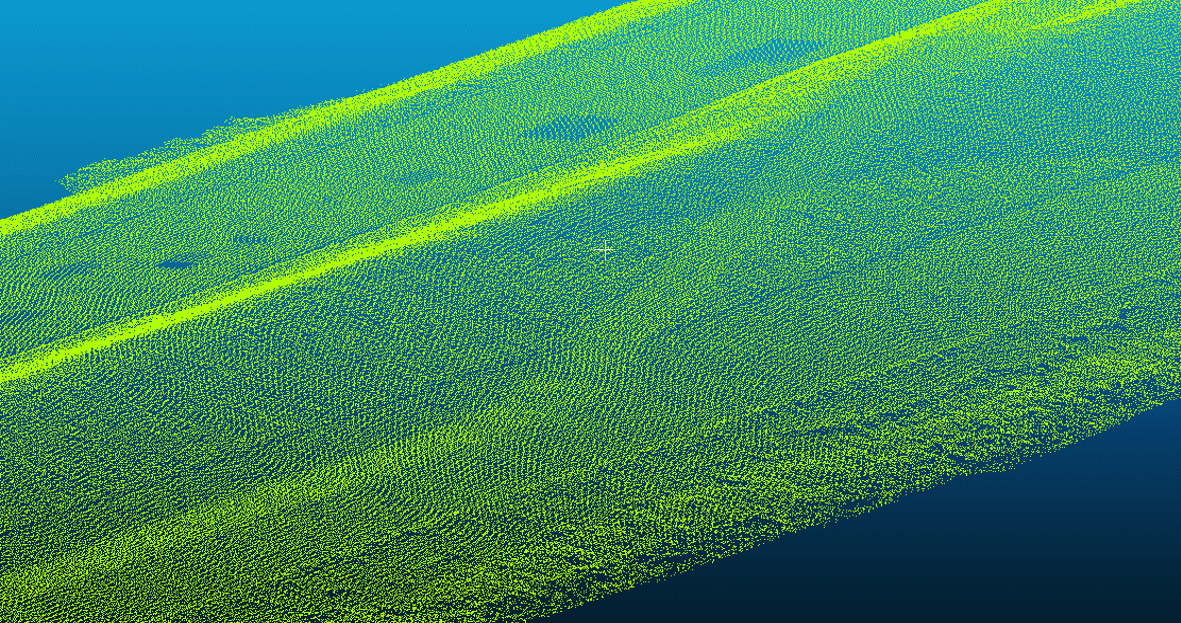
\includegraphics[width=6cm, height=3.5cm]{final_report/figs/ahn_sample_20BN1_a.png}}  \\
Amsterdam Hemhavens, \codeword{25BZ2} & Ringweg-West motorway as it crosses the IJ through the Coentunnel in a densely built-up environment. It is built on artificially elevated ground and on bridges in this area. Part of Westradweg also included, built entirely on a long bridge. & \raisebox{-0.94\totalheight}{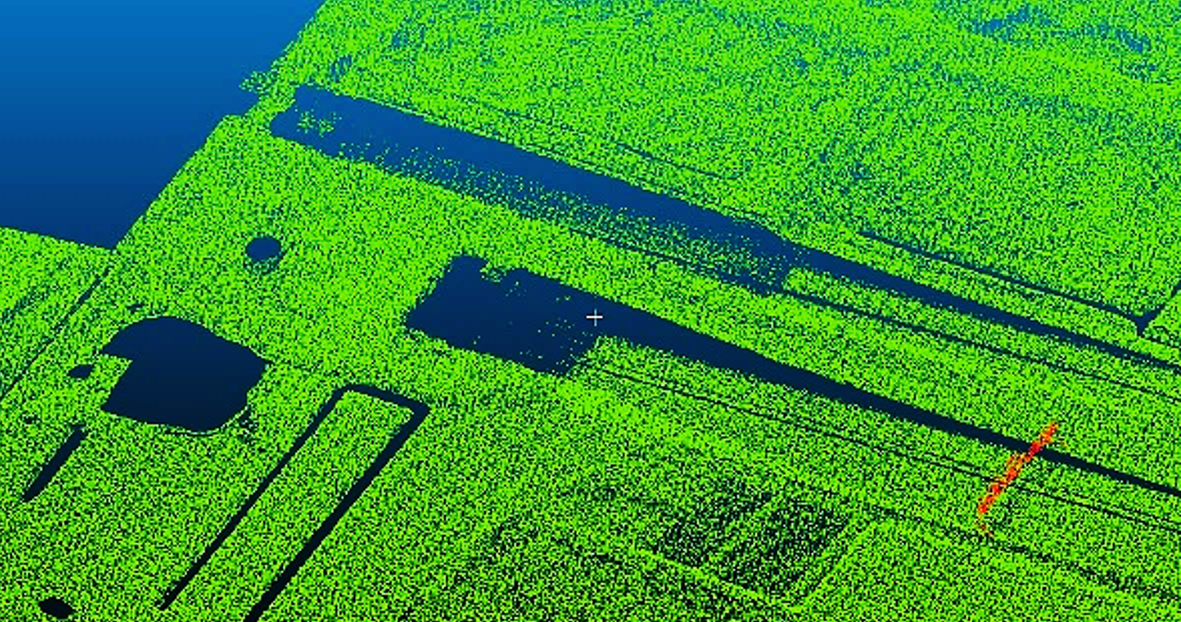
\includegraphics[width=6cm, height=3.5cm]{final_report/figs/ahn_sample_25BZ2_a.png}} \\
Amsterdam Zuid, \codeword{25DN2} & \ac{r_roads} with many closely spaced bridges, small tunnels, dense grouping of holes around roads due to presence of water and buildings & \raisebox{-0.94\totalheight}{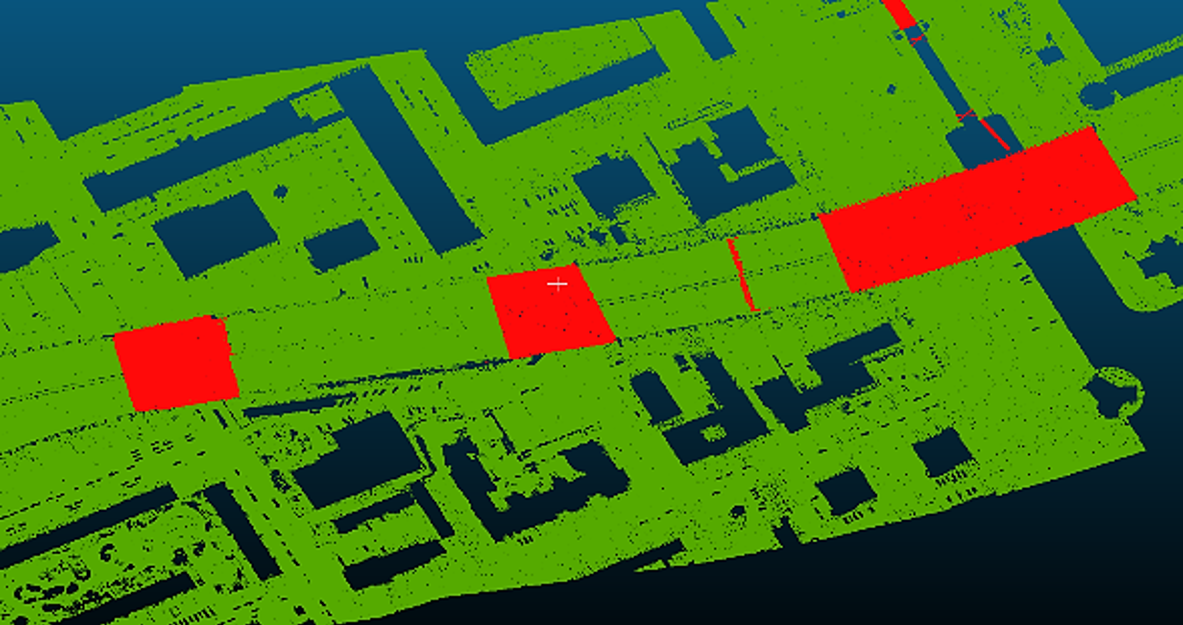
\includegraphics[width=6cm, height=3.5cm]{final_report/figs/ahn_sample_25DN2_a.png}} \\
Bunschoten, \codeword{32BN1} & \ac{p_roads} with three big roundabouts, and one road that ends in a small roundabout. Amersfoortseweg has its two lanes on separate road surfaces (like motorways), but with frequent connecting segments. & \raisebox{-0.94\totalheight}{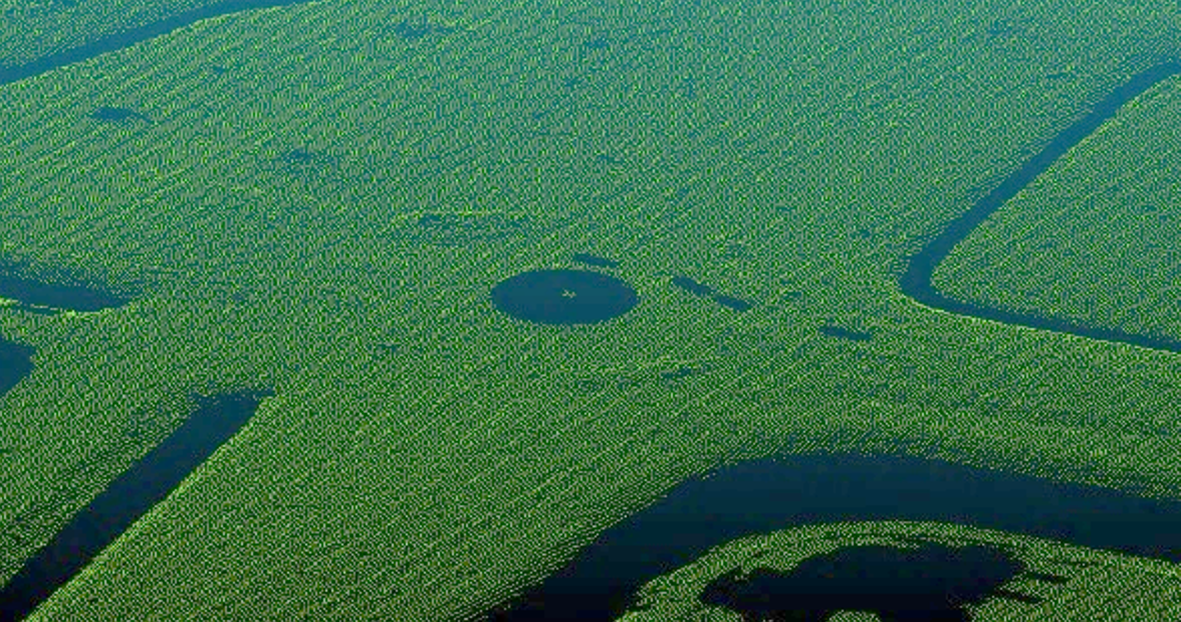
\includegraphics[width=6cm, height=3.5cm]{final_report/figs/ahn_sample_32BN1_a.png}} \\
Veluwe, \codeword{32FZ2} & Straight \ac{r_roads} surrounded by dense forest and crossed by wide wildlife overpasses. & \raisebox{-0.94\totalheight}{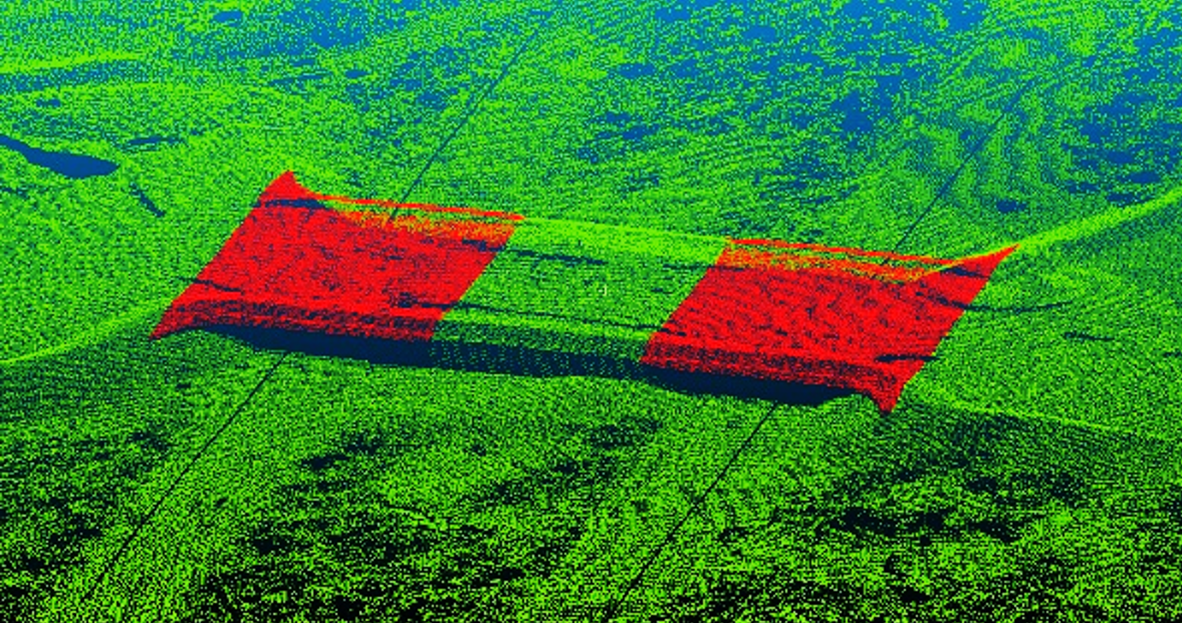
\includegraphics[width=6cm, height=3.5cm]{final_report/figs/ahn_sample_32FZ2_a.png}} \\
Apeldoornseweg, \codeword{32HZ2} & \ac{p_roads} in dense forest with canopy frequently occluding the road surface, decreasing point density and occasionally creating gaps. The road has small parallel branches running very close to it, which may make it difficult for the algorithm to distinguish between them. It also has roundabouts. & \raisebox{-0.94\totalheight}{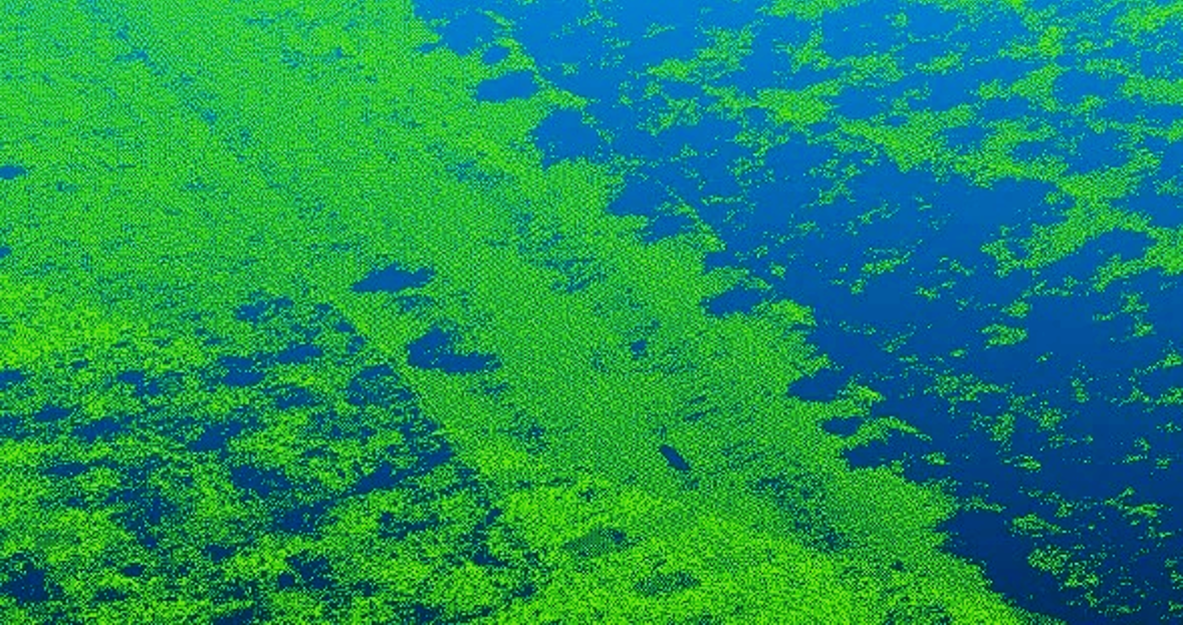
\includegraphics[width=6cm, height=3.5cm]{final_report/figs/ahn_sample_32HZ2_a.png}} \\
Hoenderloo, \codeword{33CN2} & \ac{p_roads} in extremely dense, continuous forest with canopy frequently occluding the road surface, decreasing point density and occasionally creating gaps. Both lanes are on the same road surface & \raisebox{-0.94\totalheight}{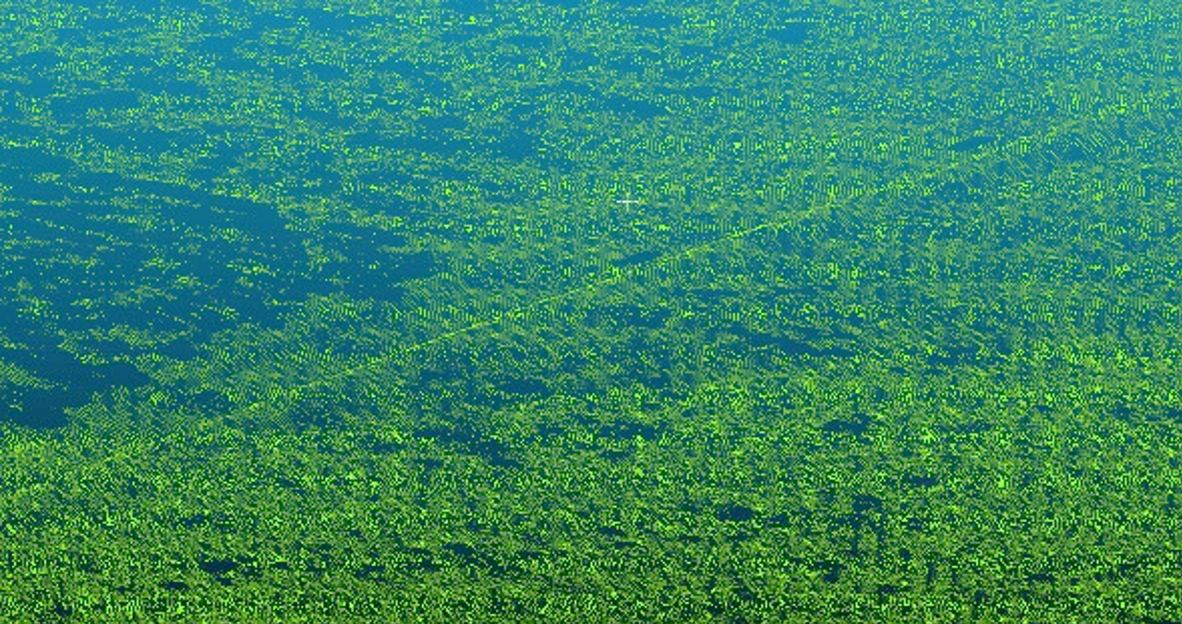
\includegraphics[width=6cm, height=3.5cm]{final_report/figs/ahn_sample_33CN2_a.png}} \\
Rotterdam Ketheltunnel, \codeword{37EZ1} & This segment of the A4 heading North from Rotterdam has been recently reconstructed in an underground tunnel. In addition, a significant portion of this motorway now runs in a trench towards Delft. \ac{ahn3} was imaged during the reconstruction, and hence contains anomalous data about the road surface. & \raisebox{-0.94\totalheight}{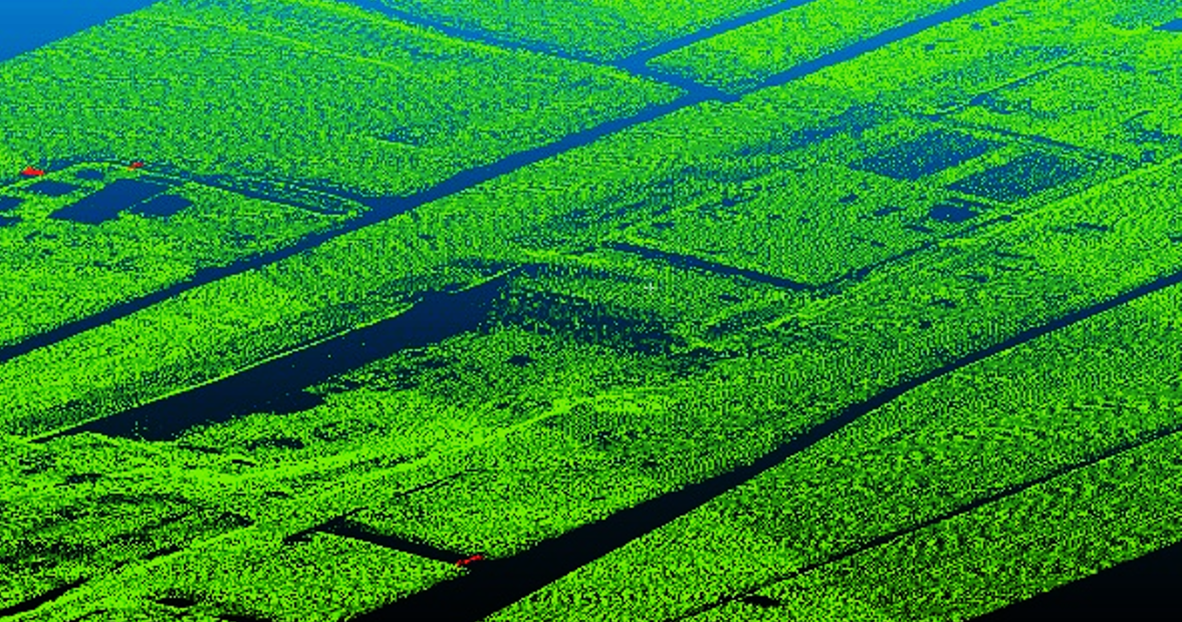
\includegraphics[width=6cm, height=3.5cm]{final_report/figs/ahn_sample_37EZ1_a.png}} \\
Knooppunt Ridderkerk, \codeword{37HN2} & The Ridderkerk junction is one of the largest of its kind in The Netherlands, in one place containing 4 overlapping \ac{r_roads}. Furthermore, it contains a high density of \ac{r_roads} in a small area, many of them very tightly packed. Many of them have very sharp bends. & \raisebox{-0.94\totalheight}{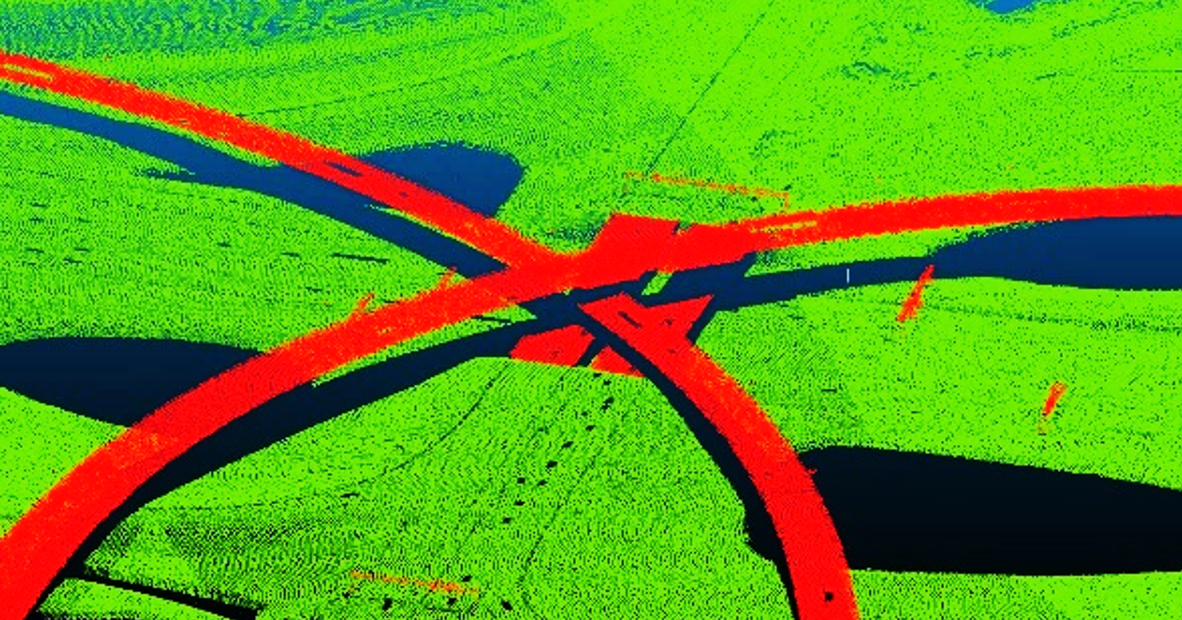
\includegraphics[width=6cm, height=3.5cm]{final_report/figs/ahn_sample_37HN2_a.png}} \\
Gorinchem, \codeword{38GZ1} & Complex junction between \ac{p_roads} and \ac{r_roads} with small ramps, roundabouts and overlapping geometries. & \raisebox{-0.95\totalheight}{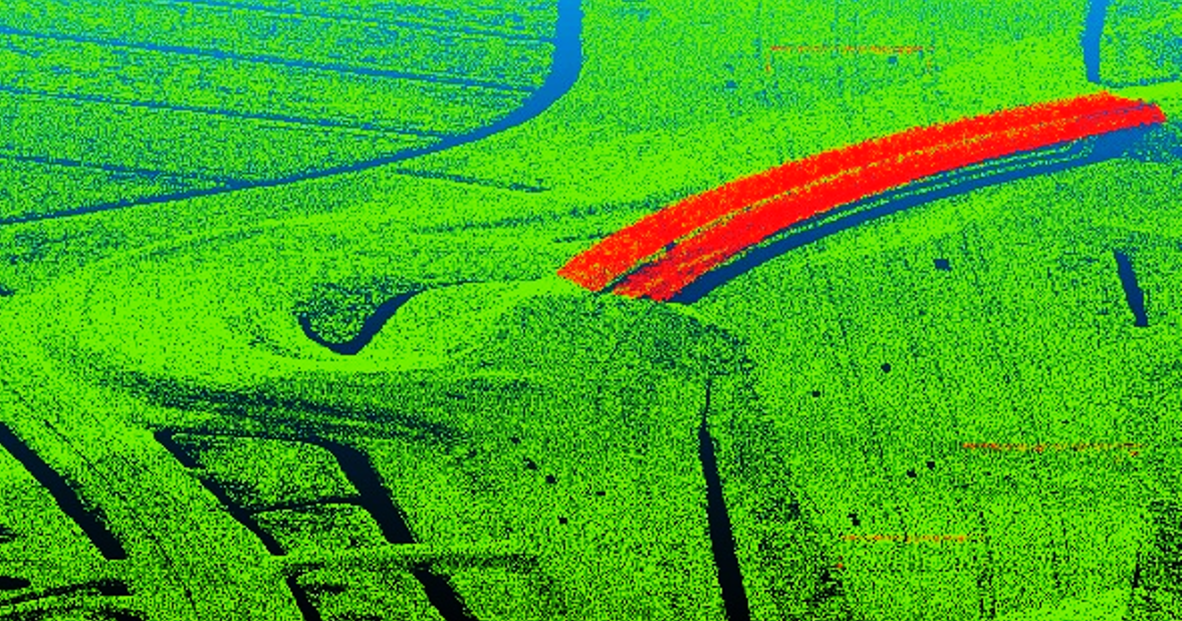
\includegraphics[width=6cm, height=3.5cm]{final_report/figs/ahn_sample_38GZ1_a.png}} \\
Knooppunt Deil, \codeword{39CZ1} & Less complex, but analogous junction to the Knooppunt Ridderkerk. & \raisebox{-0.5\totalheight}{\textit{Please refer to Figures \ref{fig:ahnbridges}, \ref{fig:ahnsigns}, \ref{fig:ahnnwb} and \ref{fig:dtbahn}.}} \\
\toprule
\caption{Inventory of testing datasets \label{tab:inventory}}
\end{longtable}

One instance of my software can process a single testing dataset at a time. However, running multiple Python instances in parallel allows one to easily parallel-process multiple tiles depending on the CPU installed in the computer. Each dataset consists of a cropped \ac{nwb} and \ac{dtb} file, and the clipped \ac{ahn3} point cloud.

All datasets mentioned in Table \ref{tab:inventory} are part of the GitHub release of the results. A compressed archive with the input testing files (and all intermediate results and final results) can be downloaded via a link found in the repository's readme file.

\section{Results of processing steps}
\label{sec:results}

The results below are presented in the same section structure as the detailed methods were in Section \ref{sec:methods} of the previous chapter. This is intended to make it easy for readers to correlate the results with the theory underlying the relevant processing mechanisms. In each section, I describe - with the help of 3D visualisations - how well each processing step performs, and how effective and useful they are in the context of the entire pipeline as a whole. I also devote attention to describing typical scenarios in which algorithms are useful and perform well, as well as ones where the opposite is true and they may produce sub-optimal results. Lastly, in each of the pipeline steps I make mention of how exactly the underlying software implementation is meant to be used, with notes on the recommended arguments.

\subsection{Splitting NWB into NBRS}
\label{sub:r_nbrsgeneration}

Each line colour in Figure \ref{fig:nbrsgeneration0} corresponds to a specific \ac{nbrs} ID, meaning that LineStrings (\textit{wegvakken}) belonging to the same \ac{nbrs} are also coloured the same. The figure demonstrates that as a result of the \ac{nbrs} generation step, the cropped road network becomes semantically enriched with identifiers linking certain LineStrings together, based on semantic or geometric conditions depending on which algorithm was used.

The colours are generally inconsistent between the results of the two algorithms (top and bottom parts of the figure). Although the same colour scheme was used to prepare them, the two algorithms distribute the \ac{nbrs} IDs differently.

\begin{figure}
    \centering
    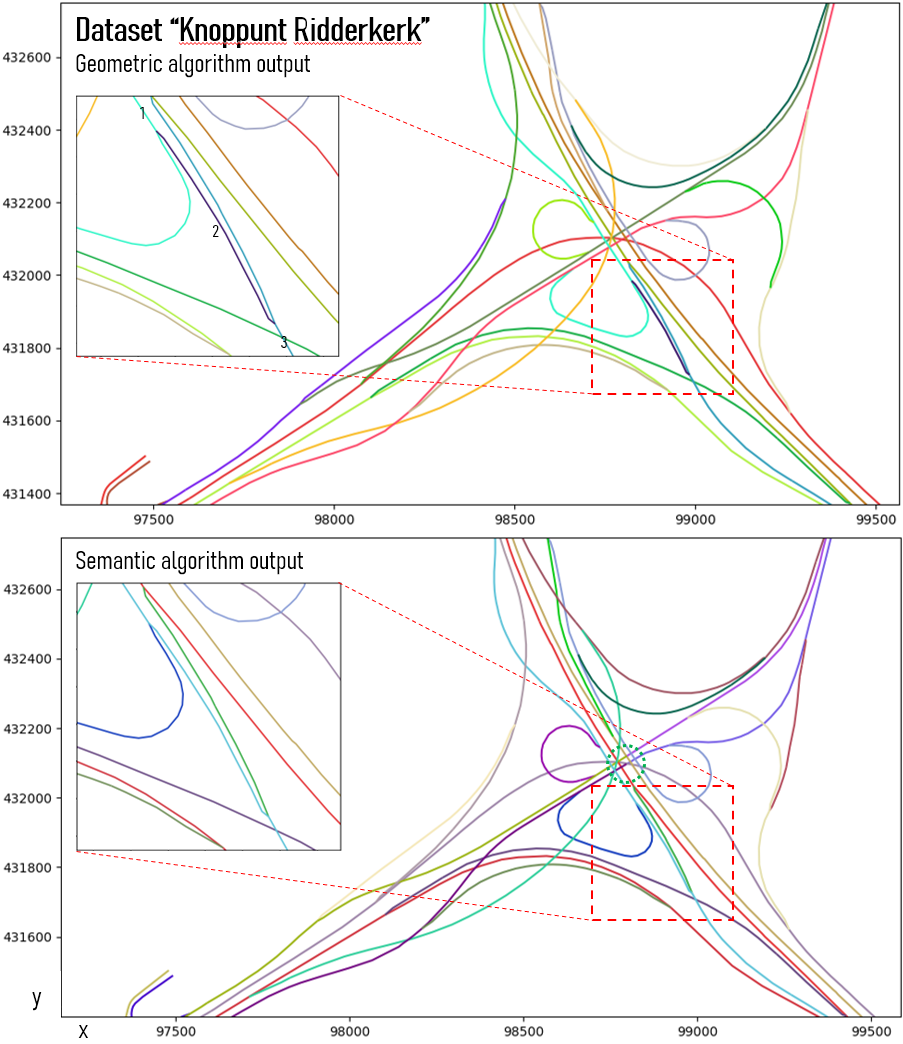
\includegraphics[width=\linewidth]{final_report/figs/nbrsgeneration0.png}
    \caption{Visualisations illustrating the results of \ac{nbrs} generation.}
    \label{fig:nbrsgeneration0}
\end{figure}

\subsubsection{Issues with geometric algorithm}

The figure also serves to illustrate the fundamental differences that exist between the results of the two algorithms. The geometric algorithm makes the assumption that the 2D georeferencing of \ac{nwb} is fully representative of the real-life geometry of road centrelines. However, I found this to be violated in various places as already mentioned in Section \ref{sub:nwb}. In short, where \ac{r_roads} intersect (this includes ramps, motorways and all combinations thereof), they often do so at abrupt angles, which can be observed in various places in Figure \ref{fig:nbrsgeneration0}, and especially in the insets. These angles are not representative of the real-life road geometry, they were drawn manually by data handlers to ensure that \ac{nwb} complies with certain external requirements. Consequently, they may prevent correct decisions from being made based on the intersection angles.

In places where the above intersection angle related problem exists, choosing the straightest continuation across an intersection when building an \ac{nbrs} does not necessarily represent the optimal choice, because the angles are artificial. This can be observed in the inset of the top chart in Figure \ref{fig:nbrsgeneration0}, where I numbered some of the \ac{nbrs} on the geometric results. While the geometric algorithm obviously made the right choice \textit{based on the pairwise angles} between the individual road segments concerned, attribute table data told the semantic algorithm that the role and road number of certain parts of \ac{nbrs} 0 and 2 are the same as that of \ac{nbrs} 1, which resulted in these parts of \ac{nbrs} 0 and 2 connecting via \ac{nbrs} 1. The "discarded" ends of \ac{nbrs} 0 and 2 then became two unique \ac{nbrs} by themselves. In the overall large-scale context of the local road network, the semantic algorithm evidently made the correct choice, even though this introduced some small, abrupt internal angles into the \ac{nbrs}.

\subsubsection{Issues with semantic algorithm}

The green dotted circle in the semantic \ac{nbrs} generation results points out a place where the role and road number of a ramp changes suddenly, outside of a real-life intersection, which results in the algorithm abruptly starting a new \ac{nbrs} there. This is indicated by a change of colour from dark to light purple. The break happens in an unfortunate location, in the middle of a multi-level junction where the continuation of \ac{nbrs} is crucial so that large-scale trends across the complicated zone may be recognised effectively in later steps. This demonstrates that while the geometric algorithm is sensitive to problems with the georeferencing of the data, the semantic algorithm is sensitive to issues with the attribute table data. Within the testing tiles I examined, the two algorithms offered a comparable amount of benefits and drawbacks.

\subsubsection{Evaluation and choice of algorithm}

Both algorithms produce usable results overall. In general, the resulting chains of \textit{wegvakken} (LineStrings) satisfy all the original requirements I set for the outputs of this step (minimise internal angles, maximise length, disallow self-intersections and branching). Based on some further testing after implementing the rest of the pipeline, I also verified that the choice of algorithm does not significantly influence the output of subsequent steps.

Since the geometric algorithm generalises to arbitrary road networks better than the semantic algorithm (i.e. does not rely on specific properties of \ac{nwb}), I used it to generate the rest of the results shown and discussed in this report.

\subsubsection{Using the implementation}

In the software, before \ac{nbrs} generation can be executed, the \codeword{nbrs_manager} class needs to be initialised with the file path to the cropped \ac{nwb} file of the desired dataset. Example calls to perform geometric \ac{nbrs} generation are provided below.

\begin{verbatim}
roads = nbrs_manager(fpath = nwb_fpath)
roads.generate_nbrs(algorithm = 'geometric')
\end{verbatim}

In the code snippet above, \codeword{nwb_fpath} refers to a variable containing the file path in the operating system to the cropped \ac{nwb} file of the desired testing dataset. For instance, the file path could end in \codeword{.../C_39CZ1_nwb.shp}, using the naming convention of the released testing files, the dataset called \textit{Knooppunt Deil} is desired. Switching to \codeword{algorithm = 'geometric'} triggers the use of the semantic algorithm.

The invocation \codeword{roads.plot_all()} may be executed to plot the results on a 2D diagram using random colours to distinguish between \ac{nbrs}. At this point, \ac{nbrs} generation results are saved in class variables only (see \codeword{roads.nbrs_wvkn}), hence running \codeword{roads.write_all()} at this point is \textbf{not} going to write the \ac{nbrs} IDs into the attribute table. The imported road network is stored in \codeword{roads.nwb} in a GeoDataFrame which also contains the generated \ac{nbrs} IDs.

\subsection{Elevation estimation}
\label{sub:r_elevationestimation}

\begin{figure}
    \centering
    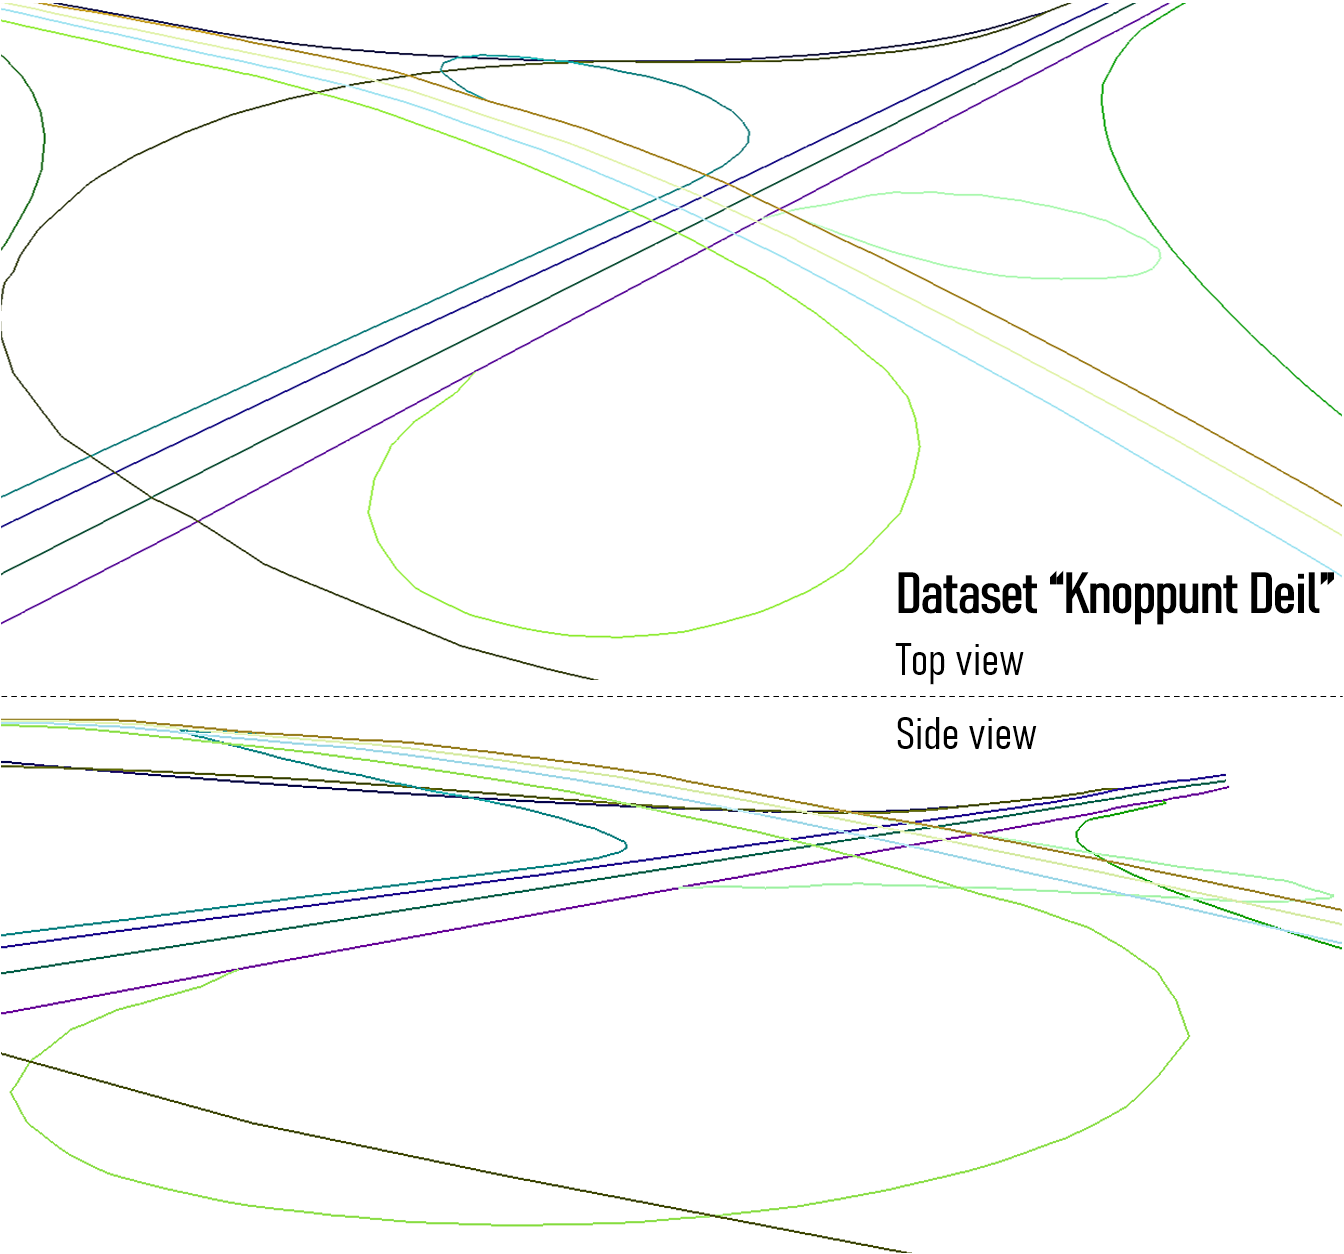
\includegraphics[width=\linewidth]{final_report/figs/elevationestimation0.png}
    \caption{Visualisations illustrating the preliminary elevation estimation results.}
    \label{fig:elevationestimation0}
\end{figure}

Figure \ref{fig:elevationestimation0} shows the results of this step in two 3D visualisations. The \ac{nwb} centrelines are shown once again in random colours based on which \ac{nbrs} they belong to, but now they are shown at their estimated elevations. The vertical dimension in this visualisation and all other 3D visualisations in this chapter are exaggerated 5-fold, so that changes in elevation are made better visible. The figure contains two visualisations that allow the reader to examine the same results from multiple viewing angles.

\subsubsection{Vertex densification}

\begin{figure}
    \centering
    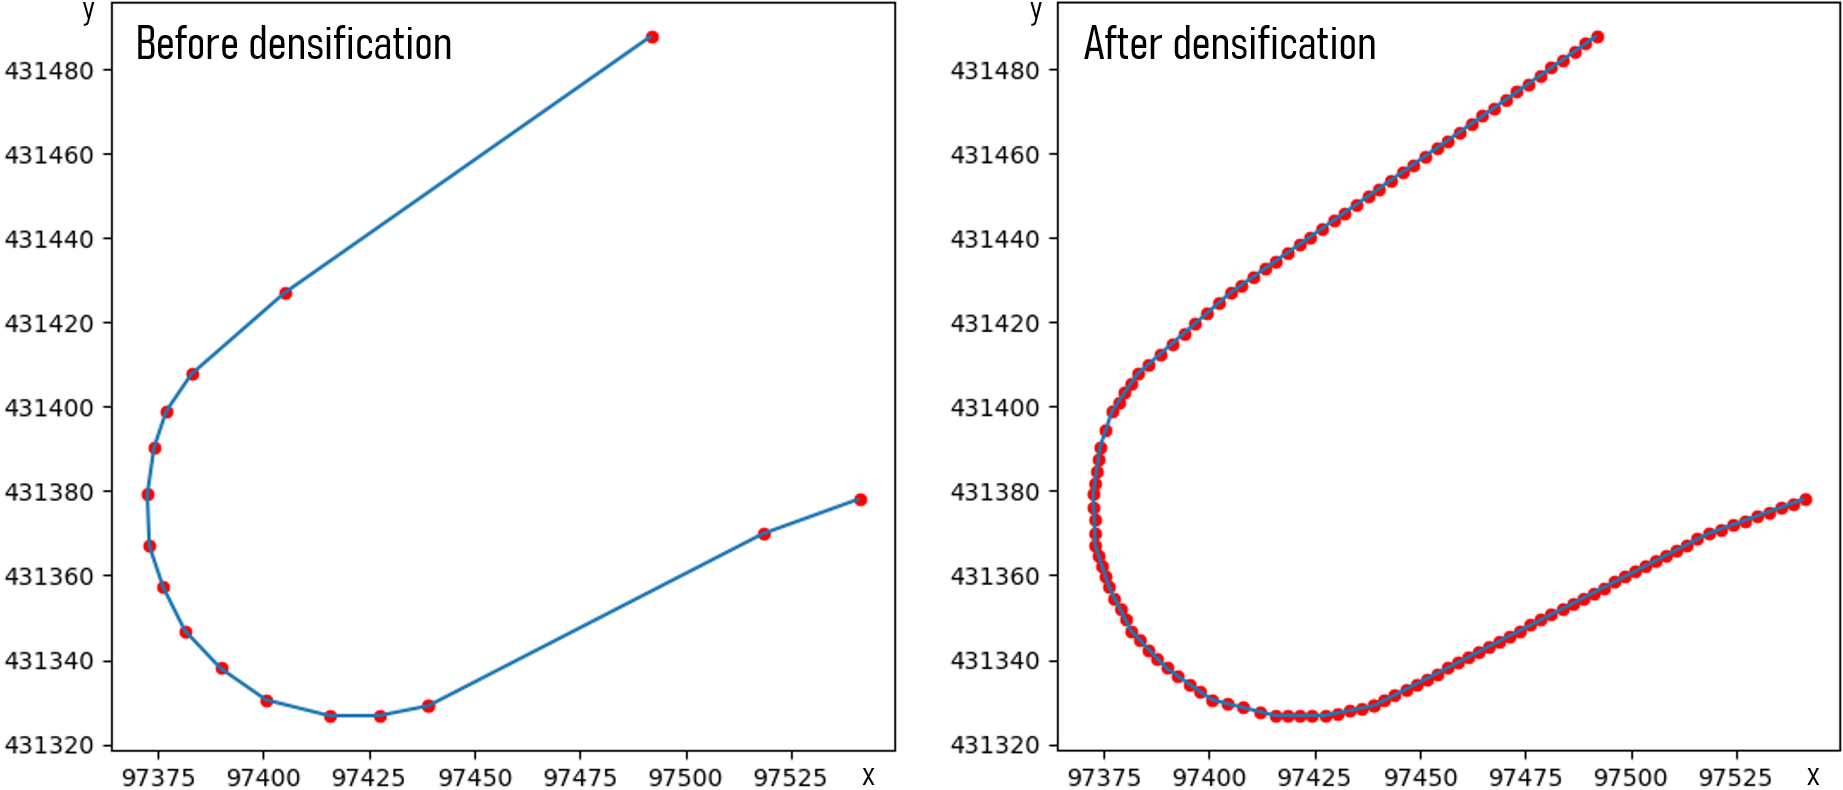
\includegraphics[width=\linewidth]{final_report/figs/elevationestimation1.png}
    \caption{Visualisations illustrating the vertex densification feature.}
    \label{fig:elevationestimation1}
\end{figure}

The vertices were densified before running preliminary elevation estimation; I used a threshold of 5 metres for the final outputs shown here. This means that no individual line segment in the 3D road network is longer than 5 metres. I found this threshold value to offer a compromise between longer processing times (in later steps) and more refined results.

We may say that while the horizontal dimensions were merely oversampled, the vertical sampling benefited from the vertex densification in the sense that it is far more detailed than it would be without them (as also mentioned in Section \ref{sub:m_elevationestimation}). An example visualisation of what happens to a specific \ac{nbrs} during vertex densification is shown in Figure \ref{fig:elevationestimation1}.

\subsubsection{Types of challenging scenarios}

Instead of focusing on details, I will only comment on the general quality of the results, since accuracy is not yet important at this step - this 3D conversion is merely a stepping stone towards the goal of performing Lidar segmentation. It only needs to fulfil its purpose in the processing workflow (to yield candidates for the subclouds), rather than to be a perfect representation of the surface. In fact, in practice it just needs to be closer to it than to any overlying points present due to occlusion.

The are two main aspects of the output that require our attention: how well the 3D centrelines conform with the real-life road surface (effectiveness of the 3D conversion), and how succesfully outliers are being eliminated (effectiveness of the refinement step). The former can be assessed via a visual comparison with the underlying \ac{ahn3} point clouds, while the latter can be examined by looking for artefacts at locations where occlusion happens. Figure \ref{fig:elevationestimation2} shows two further 3D visualisations that contain examples of the features that are relevant for this assessment.

\subsubsection{Effectiveness of 3D conversion}

The top visualisation in Figure \ref{fig:elevationestimation2} illustrates that in the case of flat lengths of roads, centrelines are generally positioned very close to the Lidar-defined road surface (within a few centimetres in general). Outliers are atypical in well-exposed areas, corresponding to the lack of outliers in \ac{ahn3} itself (and its ground classification). The procedure is fast, runtimes for the testing datasets are generally in the range of 1 to 5 seconds on a mediocre computer.

\begin{figure}
    \centering
    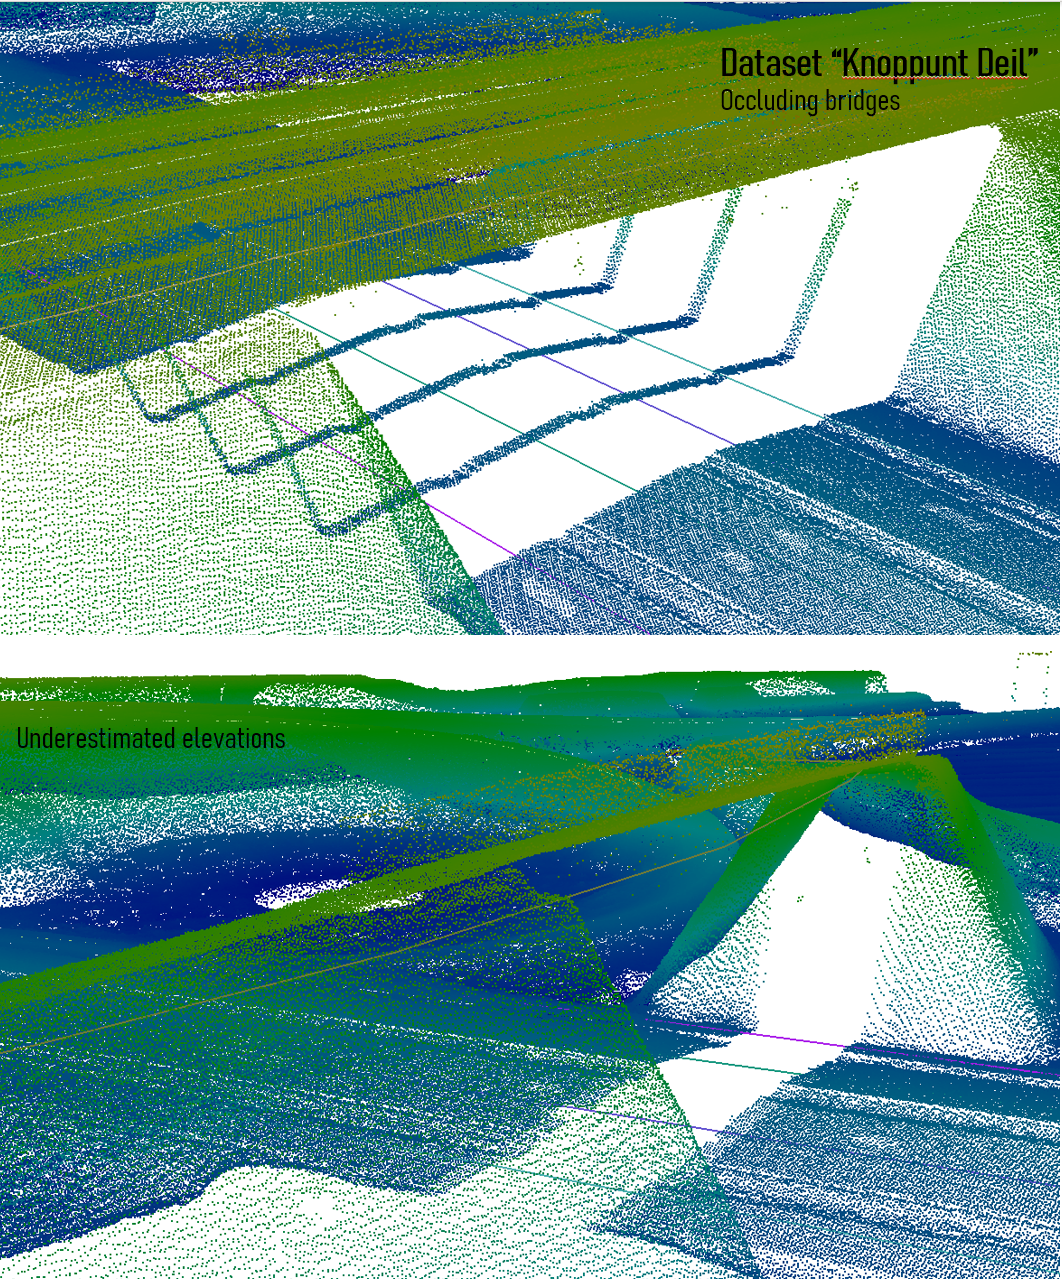
\includegraphics[width=\linewidth]{final_report/figs/elevationestimation2.png}
    \caption{Visualisations comparing preliminary 3D conversion results with the \ac{ahn3} point cloud.}
    \label{fig:elevationestimation2}
\end{figure}

Thinning the input point cloud aggressively can marginally improve the performance of this step, but it also drastically reduces its effectiveness in areas that are poorly sampled. This in turn may result in artefacts on a scale that also confuse the refinement step. I found that working with no thinning applied, or a maximum thinning factor of 3 (33\% of points kept) at most, works best. My final configuration uses a thinning factor of 2 when it imports the \ac{ahn3} data, which is carried over to all subsequent steps that work with it.

There is a range of factors that may result in the computation of anomalous preliminary elevations due to occlusion. Firstly, if an \ac{nwb} centreline is positioned far from the actual road centreline (or next to the road), then the 3D elevations will be derived from a patch of Lidar points that may include a significant number of off-road points. This may result in both positive and negative outlier elevations being computed relative to where \ac{nwb}'s georeferencing is correct. Furthermore, bridges in \ac{ahn3} include reflections from civil engineering structures, which are often attached to roads close to their edges. If the centreline of an \ac{nbrs} falls too close to the edge of the road where such objects are present, its elevations may be corrupted by Lidar points reflected from them, rather than from the road surface.

Furthermore, slow or stationary vehicles and motorway signs (due to their presence in classification 26), and larger occluding objects (e.g. bridges built \textit{over} a given road) tend to generate a sequence of outlier vertices, depending on the size of the object. Gaps in \ac{ahn3} coverage (e.g. where a road passes underneath water in a tunnel) can also give rise to missing elevations in the output of this step. Both the outlier elevations and the missing elevations resulting from these artefacts are mostly eliminated by the refinement step.

The query radius used in the KD-tree queries in my final configuration is 1 m. At the typical local posting distances found in \ac{ahn3}, this represents a compromise between fetch enough samples to minimise the effects of small-scale outliers and minimising the chances of including off road points where \ac{nwb} deviates from its optimal position. This query radius corresponds to a query area of 1 $\pi$, which typically corresponds to selecting about 30 to 120 \ac{ahn3} points in practice, depending on the local sampling density (assuming a thinning factor of 2 was used).

\subsubsection{Effectiveness of refinement step}

The effects of the refinement step can be observed in the shape of the \textit{lower} set of 3D centrelines shown in the top visualisation in Figure \ref{fig:elevationestimation2}. The series of bridges causes occlusion, meaning that Lidar coverage is intermittent for the lower set of roads, for a distance of about 70 metres. Initially (before the refinement step), the centrelines of the lower set of motorway lanes thus became snapped to the elevation of overlying roads. The resulting outliers were easily identified and eliminated by the refinement step, and new values were interpolated based on the polynomial model that was fitted on the \ac{nbrs}.

For my final outputs, I used a degree of 8 for the polynomials, and set the outlier filtering threshold to 0.2 times the standard deviation of the data-model errors in the given polynomial fit. I found that in general these parameters work best with the testing datasets. Standard deviations below 0.4 metres are artificially increased to 0.4 metres to avoid modifying elevations in roads whose conformance with the model was already found to be near-perfect. More information about the detailed processing (and thus, the exact way in which these parameters are used) in Section \ref{sub:m_elevationestimation}.

This approach proved to be an effective solution in terms of eliminating occlusion-related artefacts, it is ineffective only in places where the occluding geometry is very close to the road surface. For instance, stationary vehicles occasionally introduce outliers that are not far enough from the model to be detected in the refinement step, thereby giving rise to small spikes in the output. This does not happen frequently, and does not represent a problem in the context of the pipeline as a whole. This step also fixes any outliers caused by motorway signs, which are high enough above the road surface to be detected.

A lower limit for the outlier filtering threshold is set, in practice, by the accuracy of the polynomial fits themselves. If the value is set too low, elevations that were in fact already correct may be replaced with values from poor polynomial fits. This issue arises where the vertical curvature of the modelled roads is unusually high, such as in the overpass shown in the bottom visualisation in Figure \ref{fig:elevationestimation2}. Such curvature is difficult to approximate using polynomials, especially if the corresponding \ac{nbrs} is long and also contains other types of curvature.

Even when using a sufficiently high outlier filtering threshold, the algorithm may occasionally identify lengths of such roads as outliers and reposition them to the incorrect elevation level set by the polynomial model. I successfully bridged this relatively uncommon issue by taking it into account while implementing the Lidar segmentation workflow, which will be mentioned in the next section. Therefore, these inaccurate elevations do not represent a problem on the scale of the pipeline as a whole, because the next pipeline step is not sensitive to them. Shorter \ac{nbrs} lengths could help deal with this problem in a more explicit manner, but this would also mean that certain longer trends would become impossible to model later on.

\subsubsection{Using the implementation}

The below code snippet shows the code that I used to generate my final results.

\begin{verbatim}
roads.densify(thres = 5)
roads.estimate_elevations(fpath = ahn_fpath, r = 1, thin = 2)
roads.write_all(fpath = simpleZ_fpath)
\end{verbatim}

The first line performs vertex densification with a threshold of 5 metres. The second line performs the preliminary elevation estimation (and refinement) step, the variable \codeword{ahn_fpath} is assumed to contain a file path to the clipped \ac{ahn3} file belonging to the desired testing dataset. For instance, it could be \codeword{.../C_39CZ1_2_26_clipped.las} using the naming convention of the input files I released on GitHub. The tags \codeword{_2_26_clipped} in these file names refer to having kept only points in classes 2 and 26 (ground and bridge points respectively), and having clipped it to the extents of buffered centrelines. The variables \codeword{r} and \codeword{thin} control the query radius and thinning factor respectively, their default values are shown.

The last line of code writes the resulting 3D geometry to disk, "mimicking" the structure of the input file. The variable is named in such a way to distinguish it from the variable containing the file path where the final 3D-NWB results will be written, called \codeword{accurateZ_fpath}. This step is optional, it is intended for debugging and demonstration purposes only.

In the class itself, the results of this step are not stored in a separate variable, but are added to the GeoDataFrame representation of the input \ac{nwb} Shapefile, found in the \codeword{.nwb} variable of the \codeword{nbrs_manager} class.

\subsection{Lidar segmentation}
\label{sub:r_lidarsegmentation}

\begin{figure}
    \centering
    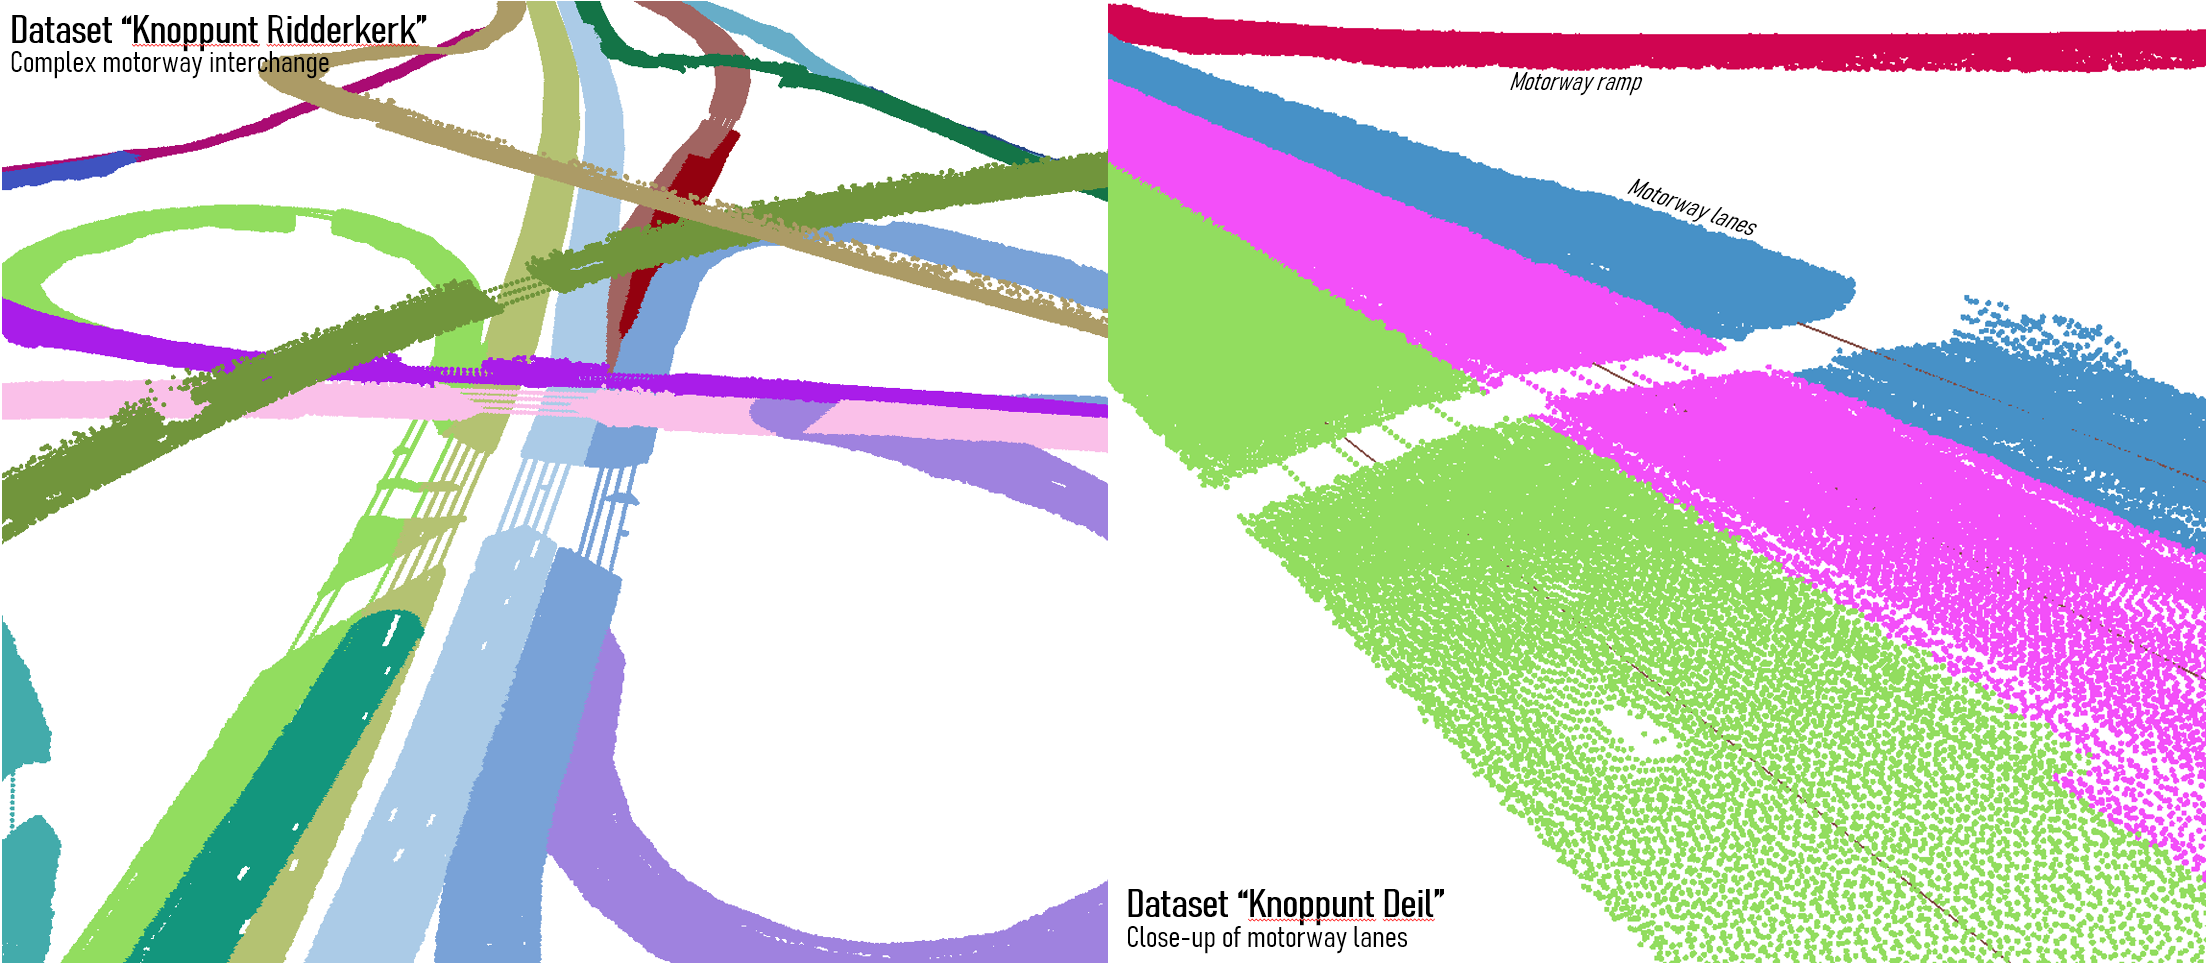
\includegraphics[width=0.86\linewidth]{final_report/figs/lidarsegmentation0.png}
    \caption{Visualisations illustrating the results of Lidar segmentation.}
    \label{fig:lidarsegmentation0}
\end{figure}

Figure \ref{fig:lidarsegmentation0} shows some visualisations of the results of Lidar segmentation. Like in figures depicting \ac{nbrs} alone (such as e.g. Figure \ref{fig:elevationestimation0}), I used colours to dinstinguish between the subclouds of each \ac{nbrs}. On the right in the figure, the centrelines are also shown (in black, to help distinguish them from their subclouds). For subclouds which are positioned far from each other, a clear separation is observable. However, ones that are close to one another often overlap, such as in various places in the centre of the visualisation on the left in Figure \ref{fig:lidarsegmentation0}. This is the result of there not being much space between the roads themselves. The overlapping parts of such subclouds may contain duplicate points (in other words, points may be part of multiple subclouds). Out of these "duplicate" points, the visualisation only shows the ones that were loaded last, hence some subclouds may appear thinner than they are.

\subsubsection{General description of results}

The properties which we are looking for in the resulting subclouds is that they contain as many of the road surface points, and as few of the surrounding unrelated points, as possible - especially with regards to points reflected from occluding objects. Figure \ref{fig:lidarsegmentation0} illustrates quite vividly that indeed, each \ac{nbrs}'s subcloud is clearly related to the underlying real-life road surface and that very few unrelated points are included.

Since this is not yet the stage where conservative thresholds are enforced, it is possible that a small amount of undesired points will be retained. This is mostly happens just before and after regions of occlusion, where the underlying plane fits have already been affected by the occlusion but not enough to be excluded. An example of such a group of points (the bottom part of a wall) is found in the blue subcloud on the right in Figure \ref{fig:lidarsegmentation0}. Reflections from tall vehicles, as well as from roadside guardrails and small signs may also be retained in this step sometimes, which explains the fuzzy appearance of the bridges on the left in the same figure.

This problem arises because the Lidar patches inevitably include off-road points, causing the fitted planes not to lie perfectly on the road surfaces. This in turn means that using very strict point-to-plane thresholds is not advisable, opening the possibility for unrelated points to make it into the subclouds. While iteratively refining the plane fits could reduce the impact of this issue, it would also introduce unnecessary computational complexity. This step of the pipeline does not \textit{need} to to produce perfect results, the small number of artefacts can be handled by later pipeline steps. 

The visualisation on the left in Figure \ref{fig:lidarsegmentation0} shows the \textit{Knooppunt Ridderkerk} motorway junction in which many motorway lanes and ramps are present in complex 3D relationships, in one place including an area with 4 overlapping roads. The correctness of the resulting subclouds demonstrates that although some of my approach is procedural and relies on a fixed parametrisation, it is still robust enough to work in the simplest, as well as the most challenging environments.

\begin{figure}[h]
    \centering
    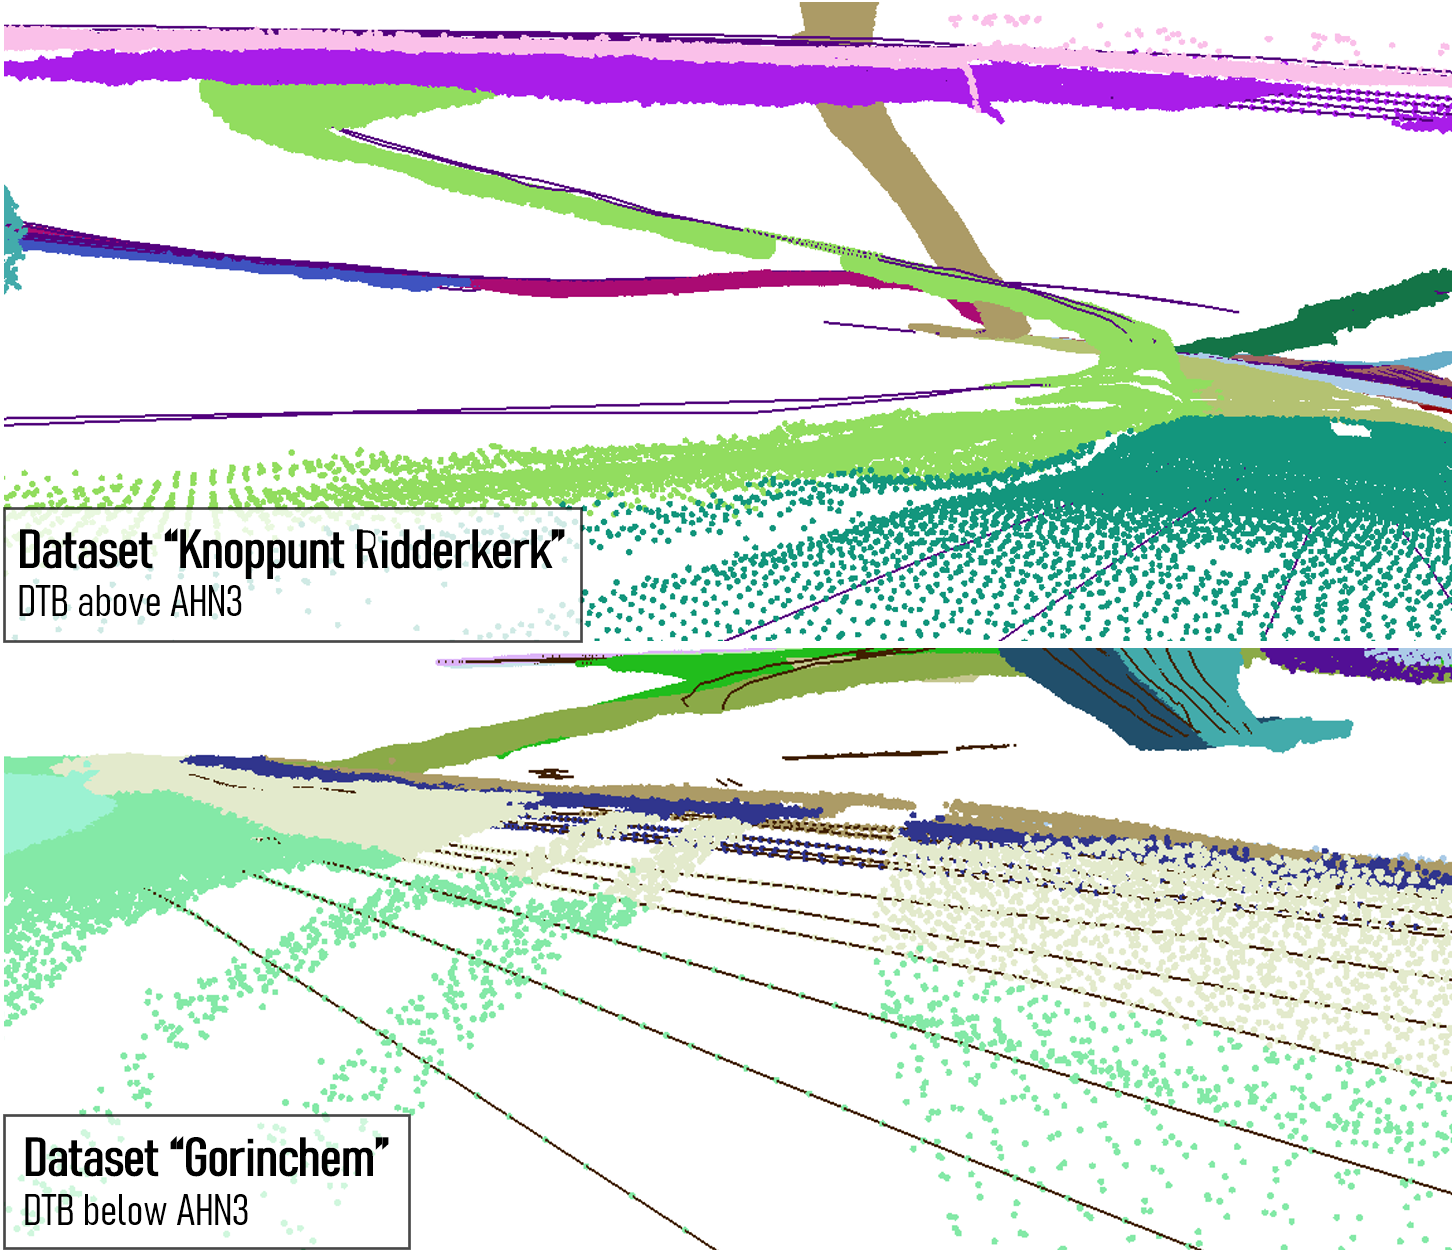
\includegraphics[width=0.9\linewidth]{final_report/figs/lidarsegmentation1.png}
    \caption{Visualisations illustrating the disagreement between \ac{ahn3} and \ac{dtb}.}
    \label{fig:lidarsegmentation1}
\end{figure}

\subsubsection{DTB's usefulness}

As discussed in-depth in Section \ref{sub:m_lidarsegmentation}, the final version of my code works regardless of the presence of long occluded regions, even without \ac{dtb} coverage. However, \ac{dtb} is still used wherever available and useful. One clear benefit is that \ac{dtb} can help rectify plane fits, thereby segmenting \ac{ahn3} more accurately in the vicinity of the gaps. Often, this automatically fixes the outlier-related issue I mentioned above in the context of slightly corrupted plane fits just before and after data gaps.

Furthermore, even in the knowledge that \ac{dtb} is severely outdated in many places (see Section \ref{sub:dtb}), it is still the only information source we have about roads where \ac{ahn3} coverage is missing. Where the break in \ac{ahn3} coverage is short and \ac{dtb} is outdated (or missing), linear interpolation prevails. However, where longer gaps are present and the road's elevation may change inside of them, \ac{dtb} prevails even if its data its outdated.

Unlike in most locations, \ac{dtb} has good coverage in the particular motorway junctions shown in Figures \ref{fig:lidarsegmentation0} and \ref{fig:lidarsegmentation1}, especially in the \textit{Knooppunt Ridderkerk} junction. Each of the visualisations in these figures contain examples of how \ac{dtb}-based "assistance" manifests itself in the output. Where subclouds contain Lidar-gaps filled with points in a linear arrangement, one can be certain that \ac{dtb} was used to re-fit planes and to supply points to the subcloud. On the left in Figure \ref{fig:lidarsegmentation0}, these linear sets of points appear in the lowest motorway lanes and ramps wherever the 3 overlying roads cast "shadows" on it, creating occluded zones of various shapes. Each level of the stack of roads has such a feature, except for the one on the top, which is not occluded by any objects.

While this demonstrates that \ac{dtb} - or any support dataset with road surface elevation measurements - can be helpful in complementing this procedure (which is otherwise based entirely on \ac{ahn3}), it also highlights one of \ac{dtb}'s weaknesses. While the areas shown in these figures have good \ac{dtb} coverage, the \ac{dtb} lines in the \textit{Knooppunt Ridderkerk} dataset are in some cases approximately two decades older than \ac{ahn3} (they are up-to-date in \textit{Knooppunt Deil}). Figure \ref{fig:lidarsegmentation1} demonstrates that there are noticeable systematic differences between the road elevations as depicted by \ac{ahn3} and \ac{dtb}.

In \textit{Knooppunt Ridderkerk}, \ac{dtb} is above \ac{ahn3} consistently, but the \textit{Gorinchem} dataset and several others show \ac{dtb} \textit{below} \ac{ahn3}. Moreover, as the top visualisation in Figure \ref{fig:lidarsegmentation1} shows, perfectly and poorly matching \ac{dtb} and \ac{ahn3} data and can often be found side-by-side, with only a few years of difference between the \ac{dtb} acquisition times. While in Section \ref{sub:dtb} I primarily attributed these problems to the effects of subsidence, a further investigation of the problem is justified based on these results. The reasons for these differences may be more complex than simply just being the result of subsidence.

This issue draws our attention to the general issue of temporal discrepancies between all our datasets - \ac{nwb}, \ac{ahn3}, and \ac{dtb}. This is further discussed in Sections \ref{sub:r_tinconstruction} and \ref{sub:r_interpolation} in the context of how it affects our results. Overall, the results suggest that even if we solely attribute the vertical land motion to subsidence, a 20 cm verical accuracy can only be guaranteed by periodically re-measuring the input elevations in both the primary and the support datasets.

\subsubsection{Splitting NBRS into parts}

On the left in Figure \ref{fig:lidarsegmentation2}, a region with neither \ac{ahn3}, nor \ac{dtb} coverage is shown. In this location, the \ac{nbrs} was split into two parts and in the figure, this is illustrated by the fact that I could highlight the subcloud on one side of the gap separately. The matching colour of the points shows that they still belong to the same \ac{nbrs}, but the program stores a separate subcloud for each \ac{nbrs} part, meaning that they are loaded as a separate MultiPoint object in the 3D viewer I used to generate these figures. \ac{nbrs} splitting also works well in general, it performs as expected.

\subsubsection{Parametrisation}

The parametrisation of this pipeline step is extensive, because many parts of the algorithm are of a procedural nature. Hence, I will dedicate some attention here to describing the final parametrisation I used to produce my outputs. Here I will not go into details about the exact way in which these parameters are used, as I have already described this in Section \ref{sub:m_lidarsegmentation} without specifying numerical values.

All parameters were derived from a process of experimentation and fine-tuning, although a good understanding of the problem, the procedures, and the properties of the input data were also essential in being able to define the parameters as well as to find suitable values for them.

Firstly, a query radius for the generation of the Lidar patches needs to be specified. I used a query radius of 10 metres, which is sufficiently long to allow most of road surface reflections to be included between centreline vertices. Using a smaller radius could, in some cases, improve the plane fitting results, but it would also cause the exclusion of useful Lidar points from the patches simply due to the spherical geometry of the query regions. While the radial queries are not perfectly suitable for this step, I did not implement a custom query mechanism because the performance of the radial KD-tree queries is needed for this step. The performance of this querying step is also heavily affected by the vertex densification threshold and Lidar thinning factor used previously; denser \ac{nbrs} vertices and a denser input point cloud means that the processing time will increase considerably.

When the program examines the Lidar patches corresponding to each \ac{nbrs} vertex, it either fits a plane and passes on the patch, only passes on the Lidar patch, or does neither. The program stops fitting planes below 2 points per square metre, and stops passing on points below 1. In this context, "points per square metre" is interpreted rather loosely, since the patches are actually based on points falling into spheres of a given radius rather than circles. However, since Lidar points are assumed to have been reflected from a \textit{nearly} 2.5D surface locally, this assumption is not unreasonable.

The next set of parameters controls the detection of "instability" while examining the succession of plane fits and underlying Lidar patches. \ac{dtb}-based assistance is attempted if any of the following conditions are met: the standard deviation of the Lidar patch's elevations exceeds 0.1 metres, the distance between the plane and the corresponding \ac{nbrs} vertex grew by more than 50\% since the previous iteration, or the median of the Lidar patch's elevations grew by more than 50\% since the last iteration. The latter two conditions are only considered if the absolute value of the underlying metrics (distance from \ac{nbrs}, median elevation) exceeds 0.2 metres.

The way the metric related to the centreline-subcloud elevation differences is enforced ensures that the occasional poor polynomial fits of the previous step do not cause problems here. Such fits cause the centreline to underestimate or overestimate the elevation of roads in a consistent manner. Making the metric detect abrupt \textit{changes} in these distances rather than simply setting a distance threshold adds enough flexibility to bridge the issue.

When \ac{dtb}-based assistance (re-fitting of plane) is attempted, the initial query radius when looking for \ac{dtb} points is 0.4 metres. If enough points were found to re-fit the plane (more than 2), then the second repositioning query is performed with the same radius as the one used in the generation of the Lidar patches (10 metres in my final parametrisation), because at this point it is assumed that the query position has been moved relatively close to the true elevation of the road surface. When deciding whether to do a final re-fit on the nearby part of the Lidar patch, the program once again uses the condition that the density of these points should at least be 2 points per square metre. Lidar points are deemed to be close if they are less then 1 metre away from the plane.

When pre-selecting the final set of conformant points from the patches, the program uses a threshold of 5\% of the query radius used in the Lidar patch queries, corresponding to 0.5 metres (from the final plane fit) in my final parametrisation. Outliers that are further away than 0.5 m from the subclouds do not violate this condition, they simply indicate that the underlying plane fit was somewhat tilted relative to the road surface.

While the post-processing operations of this pipeline step (breaking into \ac{nbrs} parts and filtering outliers) also have a few parameters, these are insignificant and are thus omitted from this discussion.

\begin{figure}
    \centering
    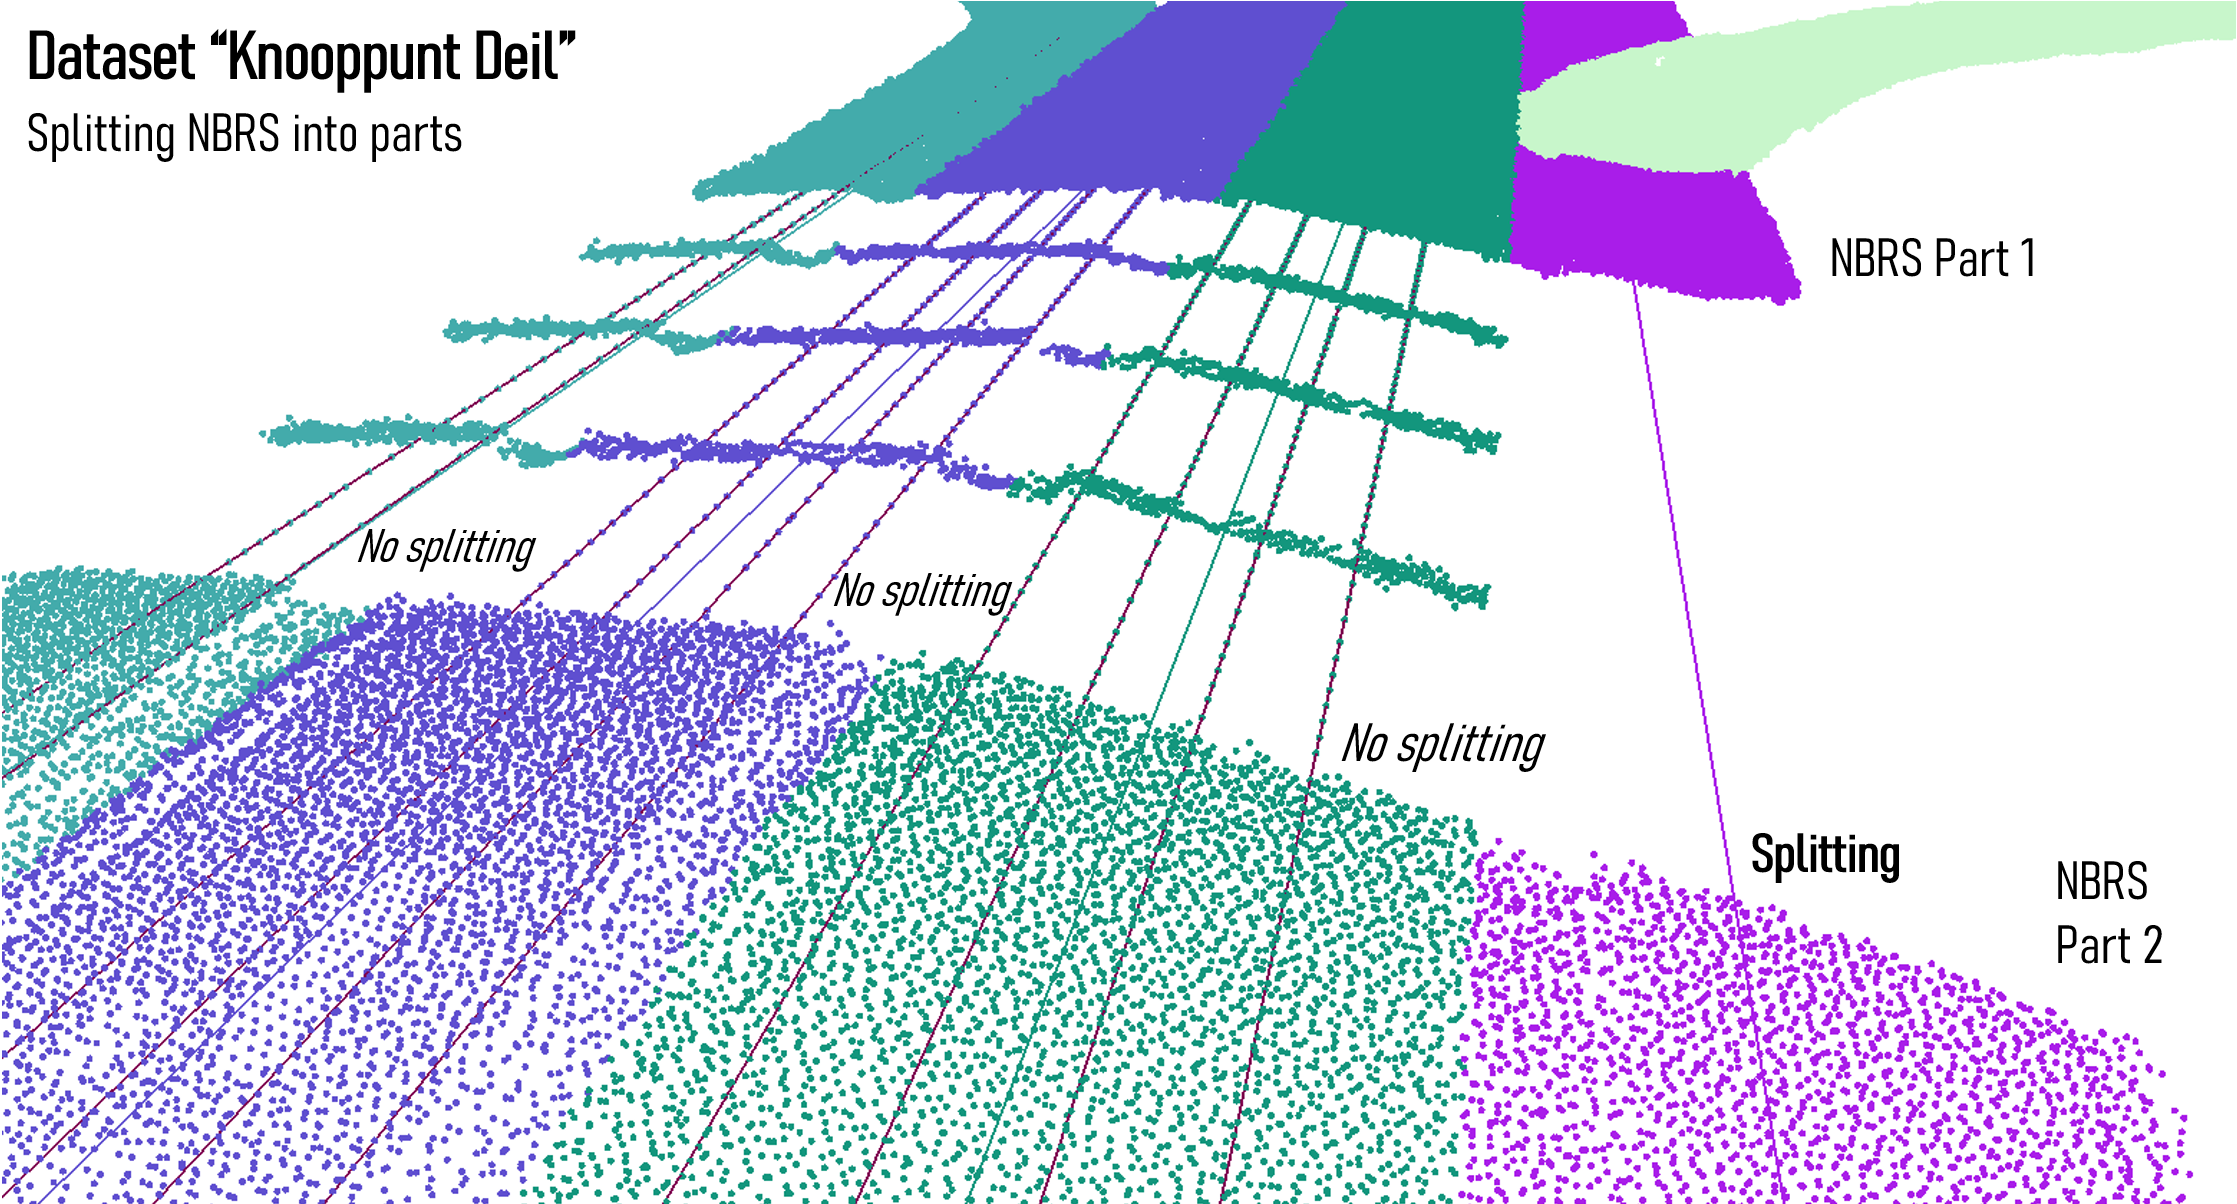
\includegraphics[width=0.92\linewidth]{final_report/figs/lidarsegmentation2.png}
    \caption{Visualisation illustrating the handling of gaps in \ac{ahn3} coverage during Lidar segmentation.}
    \label{fig:lidarsegmentation2}
\end{figure}

\subsubsection{Using the implementation}

The below code snippet shows the code I used to generate my final results.

\begin{verbatim}
roads.segment_lidar(fpath = dtb_fpath, r = 10)
roads.write_subclouds(fpath = subclouds_fpath)
\end{verbatim}

The first line performs the point cloud segmentation itself, with a radius of 10 metres for the KD-tree queries that generate the Lidar patches. The variable \codeword{dtb_fpath} is assumed to contain the file path to the cropped \ac{dtb} file belonging to the desired testing dataset. The second line writes the resulting subclouds to disk, the argument variable is assumed to contain the file path to the desired output file.

The intermediate results that the second line writes to disk "mimics" the structure of the input LAS file. However, each point is given three new properties. The property \codeword{ORIGIN} determines whether the given point originates from \ac{ahn3} (denoted by the value \codeword{0}) or \ac{dtb} (denoted by the value \codeword{1}). The properties \codeword{NBRS_ID} and \codeword{PART_ID} determine which \ac{nbrs}, and which part of that \ac{nbrs} a given points belongs to. \ac{nbrs} that were not split into parts are still represented by the same data structure, but all their points are found in a single part with \codeword{PART_ID = 0}.

In the class itself, the resulting subclouds can be accessed via \codeword{.nbrs_subclouds[nbrs_id][part_id]}, where \codeword{nbrs_id} and \codeword{part_id} are variables which should contain the ID of a specific \ac{nbrs}, and the ID of one of its parts respectively. Furthermore, one can find the indices corresponding to intervals with \ac{ahn3} or \ac{dtb} coverage in \codeword{.nbrs_parts[nbrs_id]}, which effectively defines the \ac{nbrs} parts in the software.

\subsection{Edge approximation}
\label{sub:r_edgeapproximation}

Visualisations showing the results of the edge approximation step are shown in Figure \ref{fig:edgeapproximation0}. The black lines correspond to \ac{nwb} centrelines, while the closely spaced, orthogonal lines are the cross-sections that are attempted to be created on each centreline vertex. The lines connecting the ends of the cross-sections on each side of each centreline are the preliminary edges that are the main product of this processing step. As in all 3D visualisations in this chapter, the vertical dimension is once again exaggerated five times to make vertical changes better visible.

\subsubsection{General description of results}

The output of this step is mostly satisfactory, no road layouts apart from tunnels are known to me which would cause the algorithm to fail, or produce unusable results with the final parametrisation. Furthermore, owing to the verification step that takes place before accepting a cross-section (and extending the preliminary edge with its end vertices), the general shape of the edges is also quite well-behaved, and their elevation reflects what one would expect based on the underlying subclouds. In my final configuration, cross-sections have vertices every 10 centimetres (created via densification), and their elevation is derived from points no further than 25 centimetres away. This dense quantisation allows the algorithm to reconstruct road edges on a fine scale.

\begin{figure}
    \centering
    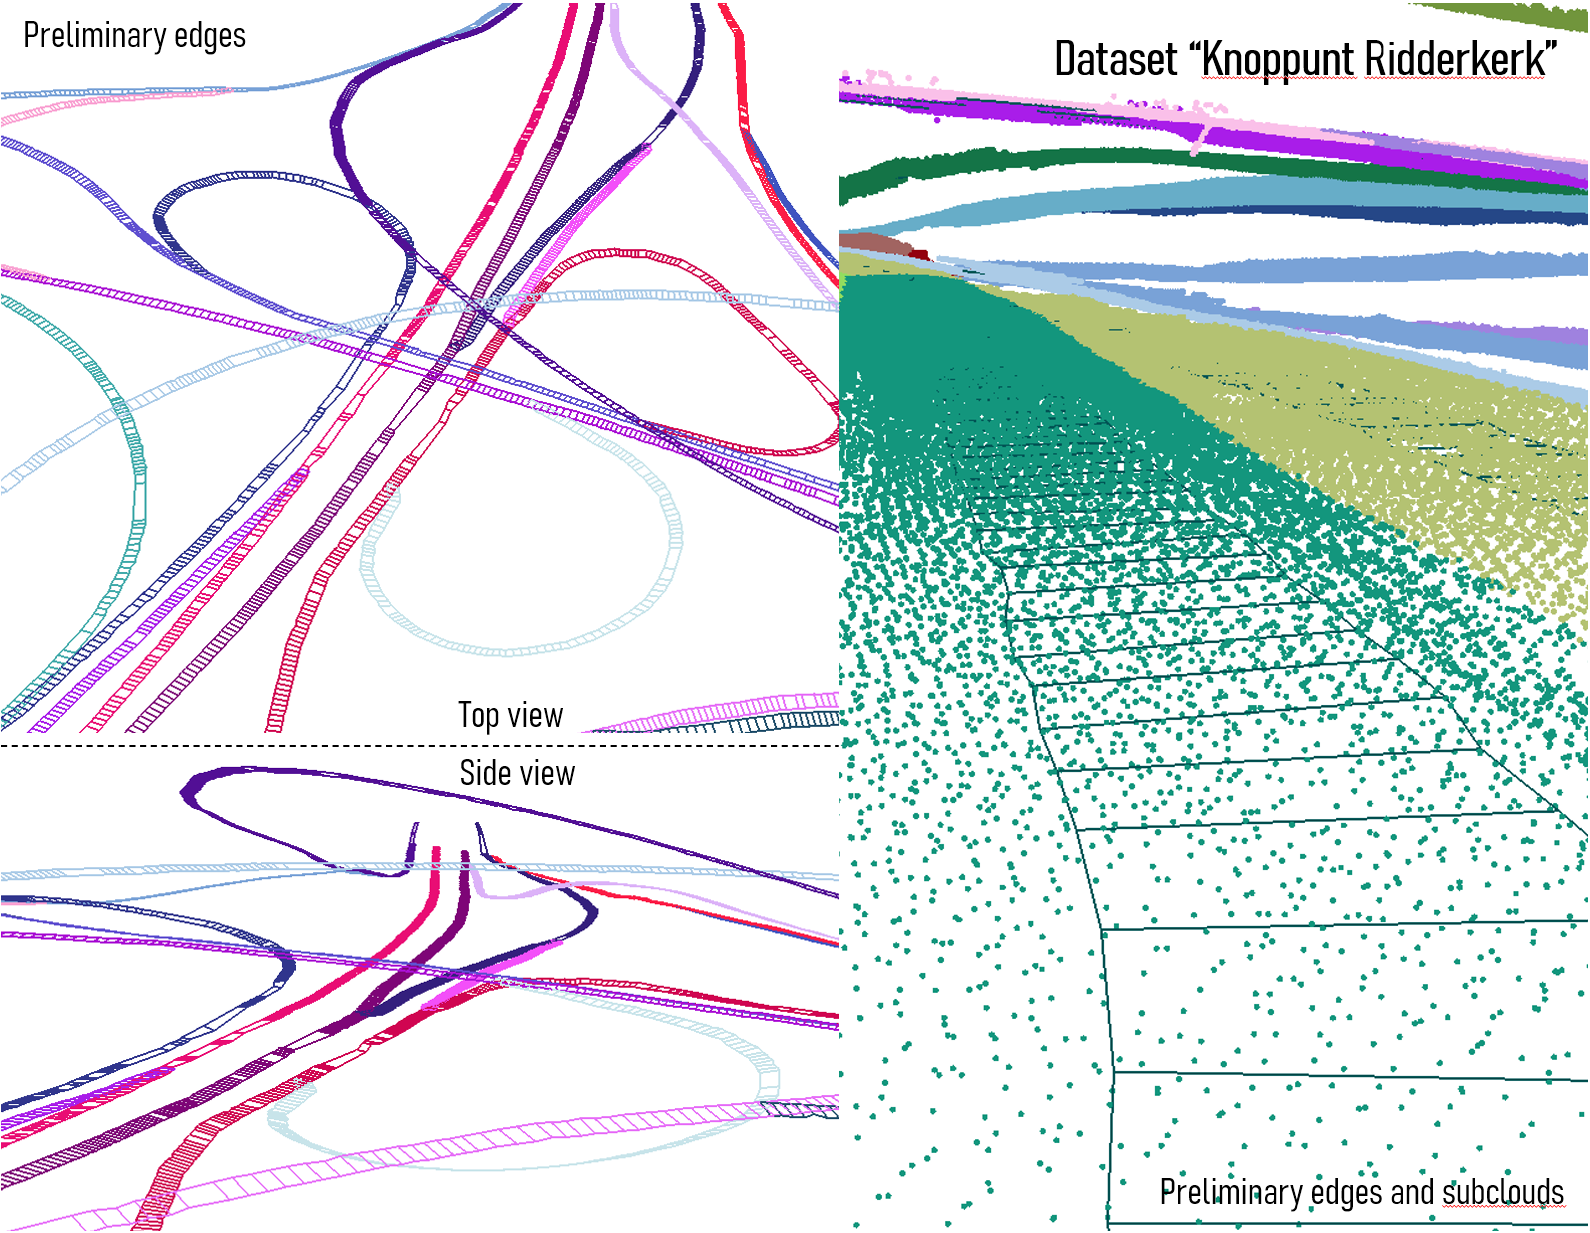
\includegraphics[width=0.9\linewidth]{final_report/figs/edgeapproximation0.png}
    \caption{Visualisations illustrating the results of preliminary edge approximation.}
    \label{fig:edgeapproximation0}
\end{figure}

In the two visualisations on left in Figure \ref{fig:edgeapproximation0}, I visualised the preliminary edges only. The top image looks down on \textit{Knooppunt Ridderkerk} from above, while the one below shows the same roads from the side. On the right in the figure, I show a visualisation in which a pair of preliminary edges and the underlying cross-sections can be compared with the subcloud that was used to generate them. In most cases, cross-sections and preliminary edges lie flat on road surfaces, and even where noticeable blunders are observed, they correspond to underestimating or overestimating the road surface extents by about 2 metres maximum.

While the overall quality is good and the results are certainly usable in terms of the requirements of the next two pipeline steps, there are a few properties and limitations of these results that are worth discussing.

\subsubsection{On road width bounds}

As I already mentioned in Section \ref{sub:m_edgeapproximation}, the algorithm works with a fixed minimum and maximum road width. The maximum is enforced by using it as the length of the constructed cross-sections, while the minimum is enforced as part of the verification step.

The enforcement of the minimum width is less of a limitation; it merely prevents the cross-sections from shrinking too short. However, the the way in which the maximum width is enforced can be considered a limitation because road surfaces that are unusually wide will not be covered by the edges in their entirety. Using very long cross-sections (increasing the maximum width) increases the chances of returning false hits due to short successions of off-road points that conform well with the line fits of the cross-sections. With shorter cross-sections, the chances of this happening are reduced drastically.

My final parametrisation uses minimum and maximum road widths of 3.5 and 7 metres respectively.

While the maximum limit may exclude meaningful road surface areas in the case of unusually wide roads, there are special roads in which road and off-road reflections are not clearly distinguishable in the cross-sections. Motorway lanes are represented by discrete centrelines in \ac{nwb}, which means they will be treated as separate \ac{nbrs} in my system. However, such lanes are often constructed on a single paved surface, meaning that my method cannot be used to derive edges at least for one side of them. This is another reason why the maximum width is important; one such scenario is shown on the left in Figure \ref{fig:edgeapproximation1}.

It is primarily \ac{nwb}'s crude georeferencing that necessitates the use of a lower-than-optimal value for the maximum road width. If \ac{nwb} itself is shifted towards the edge of a road locally, generated cross-sections will be corrupted there by off-road elevations. Using larger values for the maximum width will only make this problem worse. In the absence of this problem, the value could be increased by a few metres based on my experience with accurate parts of \ac{nwb}.

I implemented a workaround that mitigates the effects of this issue. The line fits that are generated for every cross-section are actually only fitted on the central 40\% of the densified cross-section vertices, and it is extrapolated to the outer vertices. This helps minimise the effects of the off-road elevation measurements that may affect the outer cross-section vertices. 

\subsubsection{Failed edge detection}

\begin{figure}
    \centering
    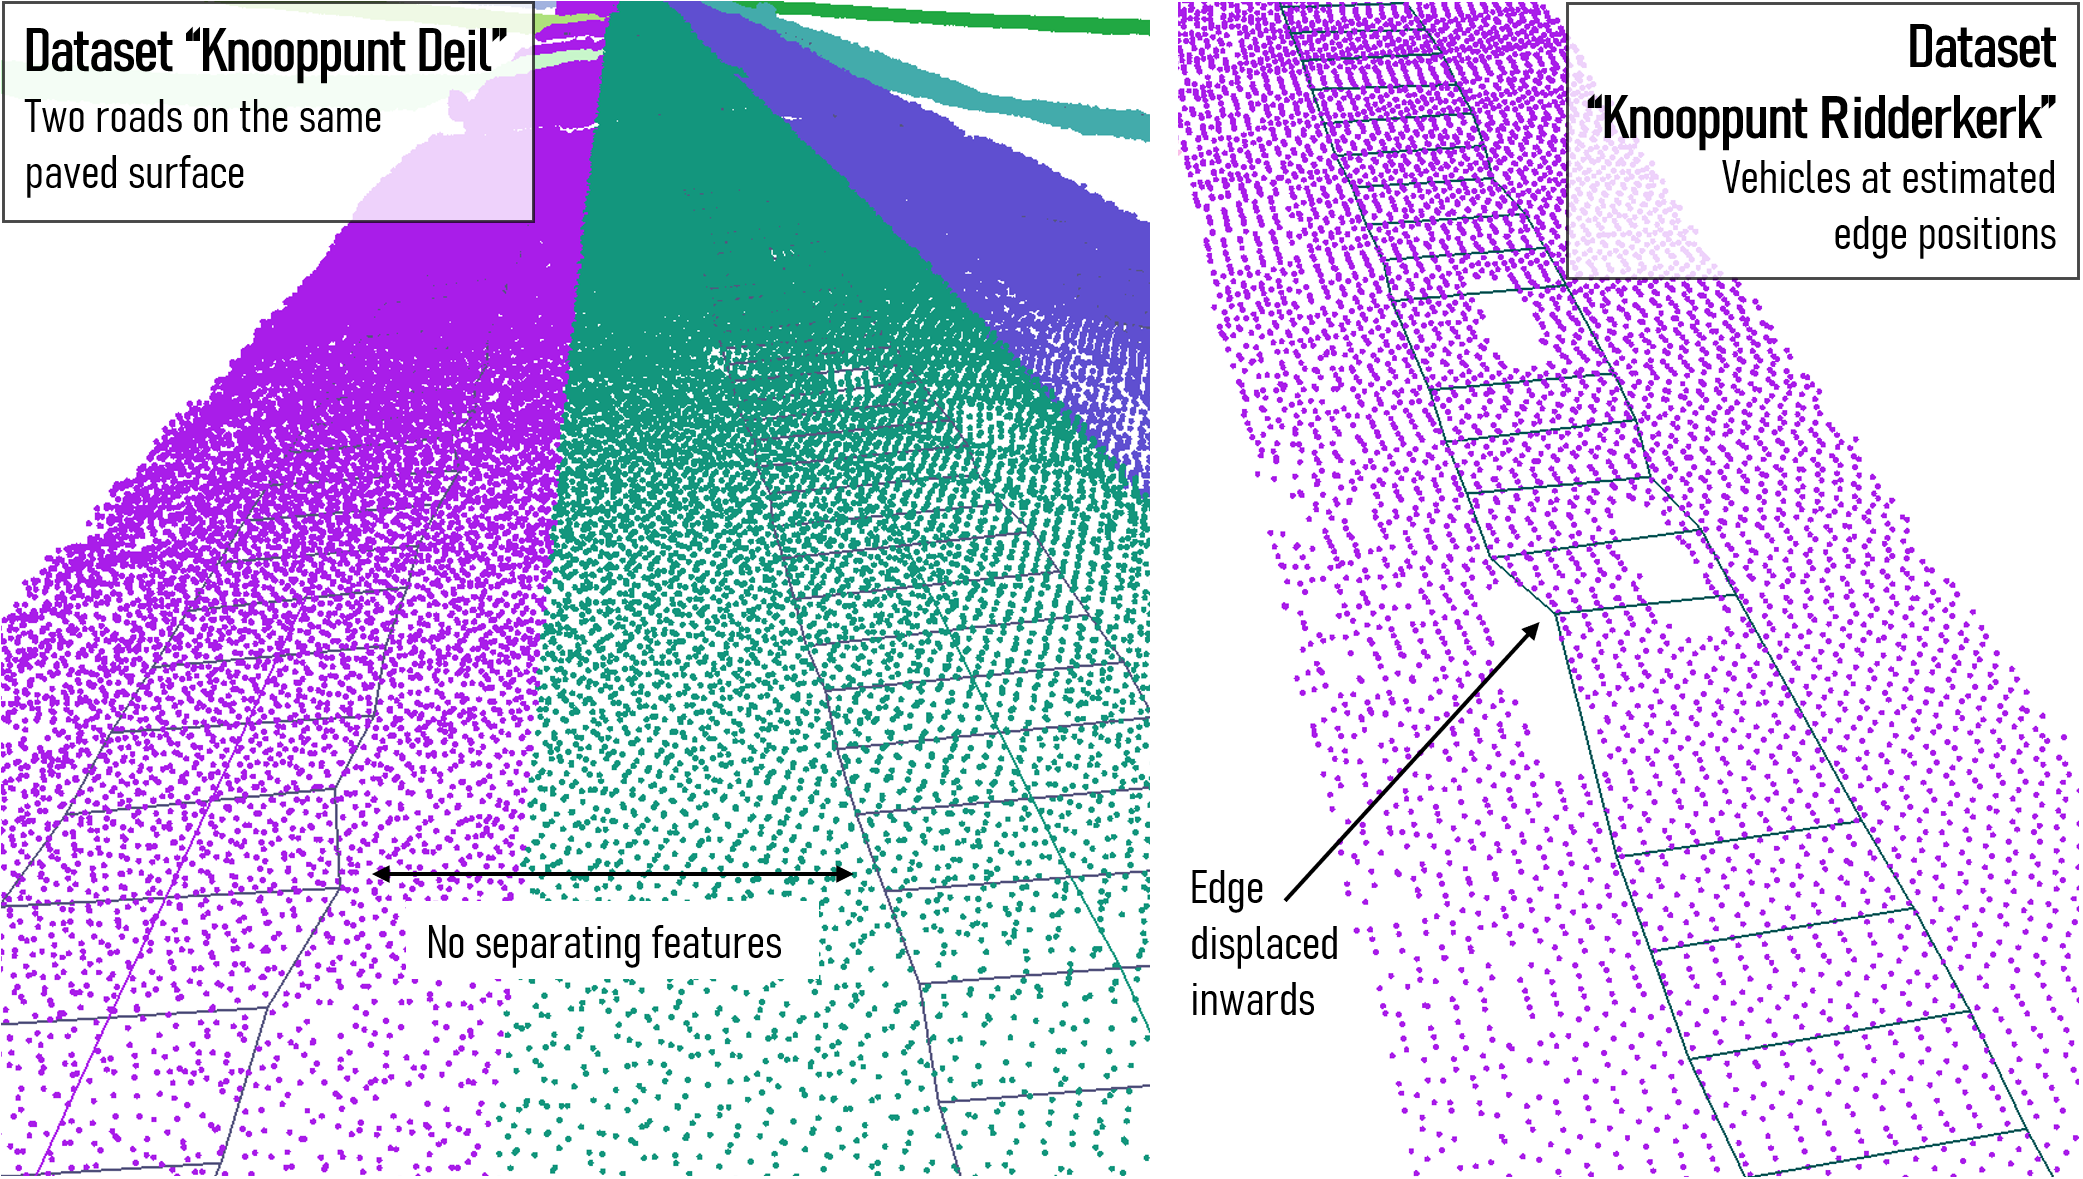
\includegraphics[width=\linewidth]{final_report/figs/edgeapproximation1.png}
    \caption{Visualisations illustrating challenging edge approximation scenarios.}
    \label{fig:edgeapproximation1}
\end{figure}

While in well-exposed, straight roads this does not generally happen, there are lengths of roads where finding edge points will fail repeatedly. In such places, the algorithm does not save the cross-sections, and also does not add edge points to the preliminary edge LineStrings. One the left in Figure \ref{fig:edgeapproximation0}, this can be clearly observed, as it occurs frequently in occluded areas.

The most common reason for skipping cross-sections is the lack of data. If not enough Lidar points are found close to the cross-section vertices, then it will be skipped. This happens in data gaps where both \ac{ahn3} and \ac{dtb} are missing, but \textit{also} in most gaps where \ac{dtb} is available. The latter is due to the fact that \ac{dtb} samples linear features \textit{along} the length of each road, and has a poor sampling rate in the direction that the cross-sections are attempting to sample.

Such data gaps may exist under bridges for instance, but also in places where vehicles occluded a significant portion of the road. In the latter case, artefacts may be generated if the cross-sections are accepted because there is enough data not to trigger a skip. Most commonly, it causes noticeable width changes, which may be accepted by the algorithm if the relevant cross-section is processed while the conditions are relaxed due to repeated previous failures. This is shown on the right in Figure \ref{fig:edgeapproximation1}.

The second most common reason is the generation of poor line fits. If the elevation estimates of the cross-section vertices are scattered, the errors in the fit will be large. Elevations further than one standard deviation of the data-model error are not considered any further. If too many points are filtered out in such a way, the cross-section will be skipped. This happens most commonly due to \ac{nwb}'s poor georeferencing, i.e. in the rare cases when not even only using the central 40\% of the cross-section vertices could avoid including a large number of off-road elevation measurements.

Lastly, failures may also be the result of violating the conditions of the verification step. Namely, if a unrealistically sudden width or elevation change is detected, the cross-section is skipped. If this is the sole reason for the failures, then generally only a limited number of cross-sections and corresponding edge vertices will be missing, as the conditions are relaxed after 3 successive failures.

\subsubsection{Edge generation in data gaps}

In the absence of \ac{ahn3} data, vertices will be skipped frequently, as I already mentioned above. However, quite frequently, one or two cross-sections will be accepted in such regions too, if \ac{ahn3} coverage reappears temporarily, for instance due to a small gap between two bridges. Due to the repeated skipping of vertices, the conditions will almost certainly be relaxed most of the time, and hence sudden width or elevation changes will be allowed. This combination of factors may result in the generation of strange edge geometries in occluded zones.

Where roads are straight and the gaps in coverage are short, this does not represent a major issue. Even if their shape will be sub-optimal in these zones, it will still respect the minimum road width condition, meaning that most \ac{dtb} and \ac{ahn3} points that may appear in the gap will still fall between the edges, which is ideal for \ac{tin} construction.

Serious problems only arise when the gap appears at the end or the beginning of an \ac{nbrs} part. In such cases, especially if there is no intermittent \ac{ahn3} coverage in the gap, no cross-sections will be accepted at all, and therefore the program will be unable to extend the edges to the end of the \ac{nbrs} part. The beginning or the end of the centreline will simply not be covered. Later in the \ac{tin} construction step, this means that the local \ac{dtb} points will not be inserted into the \ac{tin} (because they are not between the generated edges), and the \ac{tin} surface will, as a result, also not extend all the way to the end of the \ac{nbrs} part. This directly introduces incorrect (linearly interpolated) elevations to the final 3D-NWB output.

A similar problem arises when a road is occluded in a bend. Depending on the sharpness of the bend and the extent of the occlusion, the preliminary edges may end up directly connecting the last cross-section before the occlusion and the first one after. Taking such a "shortcut" means that \ac{dtb} points in the data gap will mostly be ignored during \ac{tin} generation because they will not fall between the preliminary edges.

I have not observed the above limitations to cause issues with roads that are built on the surface in practice. However, they do mean that my system design is not compatible with tunnels out-of-the-box. Unless the tunnel is completely straight and the relevant \ac{nbrs} part continues across its full length, the \ac{dtb} points in the tunnel will be ignored during \ac{tin} construction, and therefore the \ac{tin} models and the 3D conversion of \ac{nwb} will be incorrect locally. I tested and verified this issue with the \textit{Amsterdam Hemhavens} and \textit{Amsterdam Zuid} testing datasets, which both contain tunnels.

As I noted in Section \ref{sub:dtb}, I treat \ac{dtb} as a "placeholder" for a better supporting dataset (optimally, an \ac{mls} dataset). As a result, its vector properties are not used - it is assumed to consist of generic point data. However, treating it properly as a 3D line dataset in \ac{ahn3} data gaps would fix the above issues, i.e. it would become possible to generate edge estimates from \ac{dtb} much like in the commercial implementation. Such an extra feature did not fit into the schedule of my project, hence it is only further discussed in the Future work section in the Conclusions chapter (see Section \ref{sec:futurework}).

\subsubsection{Using the implementation}

In my example code on GitHub, I use the following two lines to generate and export the preliminary edges:

\begin{verbatim}
roads.estimate_edges(min_width = 3.5, max_width = 7, thres = 1, perc_to_fit = 0.4)
roads.write_edges(fpath_edges = edges_fpath, fpath_crosses = crosses_fpath)
\end{verbatim}

The first line generates the preliminary edges. The arguments (all compulsory) set the minimum and maximum road width, the outlier filtering threshold, and the ratio of how much of the cross-sections should be fitted with lines. The first two arguments should be specified in metres. The second argument specifies the number of standard deviations of data-model errors, within which points should be considered inliers, so the current value means one standard deviation. The last argument accepts values between 0 and 1, the current value means that the central 40\% of cross-sections will be used as the basis for the line fits.

The second line writes the results to disk. Both the edges and the cross-sections are written, \codeword{edges_fpath} and \codeword{crosses_fpath} are assumed to contain file paths where these should be written (as Shapefiles). In the class itself, the results are found in \codeword{.nbrs_edges} and \codeword{.nbrs_crosses} as GeoDataFrame objects.

\subsection{Active contour optimisation}
\label{sub:r_activecontours}

As Figures \ref{fig:activecontouroptimisation0} and \ref{fig:activecontouroptimisation1} show, all planned parts of this pipeline step output the expected results, albeit with occasional artefacts and a mediocre overall quality. The contours are smooth, they generally reflect the shape of the roads accurately, and only occasionally suffer from major blunders. However, even small deviations beyond the road edges would cause off-road Lidar reflections to be classified as road points, and thus be inserted in the \ac{tin} model in the next step. Unfortunately, such deviations of various sizes occur frequently, as the close-up images in Figure \ref{fig:activecontouroptimisation1} demonstrate. With the help of the results, this section will focus on explaining why exactly it is difficult to guarantee that this workflow functions reliably, as this was the reason for a major revision of the design of the preliminary edge detection and \ac{tin} construction steps, which I already mentioned in Section \ref{sub:m_edgeapproximation}.

\begin{figure}[h]
    \centering
    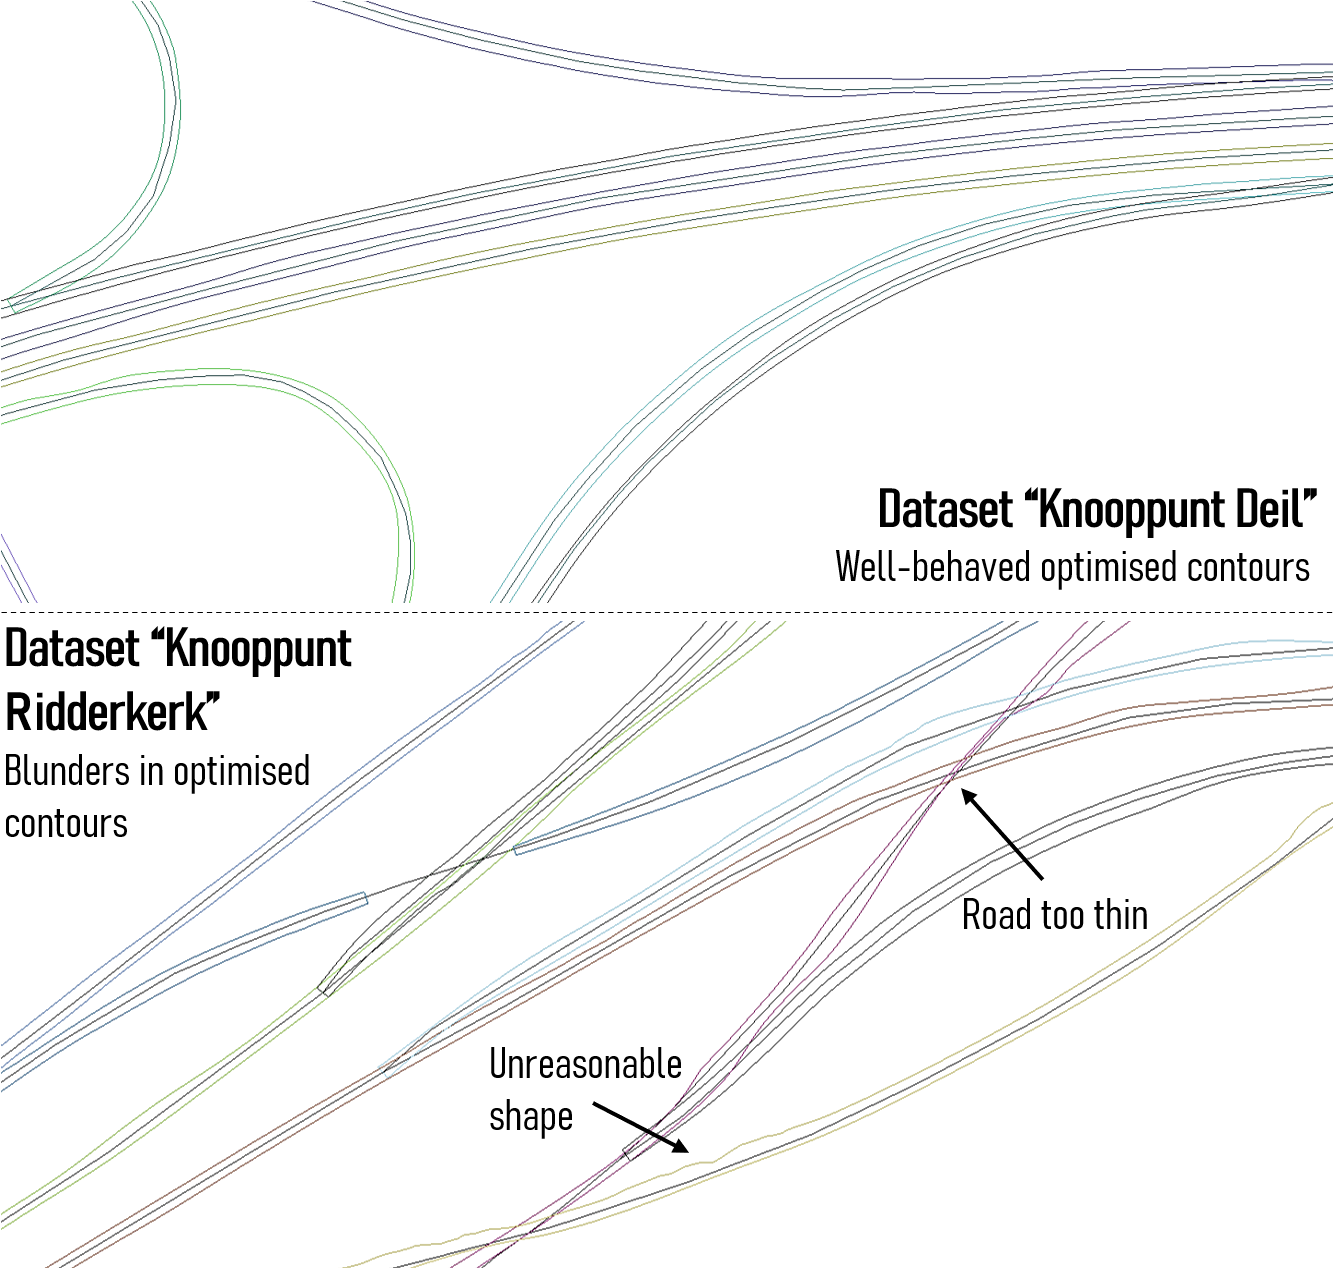
\includegraphics[width=0.84\linewidth]{final_report/figs/activecontouroptimisation0.png}
    \caption{Visualisations illustrating various degrees of active contour optimisation success.}
    \label{fig:activecontouroptimisation0}
\end{figure}

\subsubsection{Attractor maps}

Some attractor maps can be seen in Figure \ref{fig:activecontouroptimisation1}. Each \ac{nbrs} part has its own attractor map, and since subclouds may overlap, so can the attractor maps. In the figure, attractor maps that are separated from others by a fair amount of distance can be examined in their full width, while only the one the was drawn last by the visualisation software can be examined completely where overlapping occurs.

The bright parts of the attractor maps correspond to regions were the normal vectors of the Lidar points are oriented uniformly, while the darker regions indicate divergent normal vectors. The linear boundary between such regions thus marks the edge of the smooth road surface in most places, as it corresponds to an abrupt increase in normal vector divergence. I used a pixel size of 0.5 metres (in both dimensions) to generate these attractor maps, and the attractor map values are based on using a 5-by-5 kernel, sampling the neighbourhood via approximately 30 inner products for each pixel.

The optimised contours are shown overlain on the attractor maps on the right in Figure \ref{fig:activecontouroptimisation1}. While the \textit{general} appearance of the contours is acceptable, comparing \textit{details} in the contours with the attractor maps reveals that they are not reliably positioned on the break in smoothness. So that the reader can better interpret the optimisation as a process, the left part of Figure \ref{fig:activecontouroptimisation1} shows the preliminary edges overlain on the attractor maps. Comparing the preliminary edges to the contours in the context of the attractor maps allows one to better understand the effects of the optimisation procedure. In particular, patterns in the behaviour of the optimisation procedure may be recognised.

\subsubsection{Patterns of failure}

One important pattern is that the contours are sensitive to small-scale features in the preliminary edges. A few outlier edge points (an short, abrupt expansion of the preliminary edges, for instance) can introduce large bulges into the optimised edges. Similarly, where the preliminary edges shrink (for instance due to the influence of stationary vehicles), the optimised contours will tend to do so too, but on a much larger scale. The severity of the generated artefacts also depends on the local properties of the attractor maps.

Another pattern, which I already mentioned in \ref{sub:m_activecontours}, is that where preliminary edges fall outside the bright part of attractor maps, the the optimisation procedure will often fail to move them back to the primary break in smoothness. The off-road areas may contain other high-contrast features due to the unevenness of the underlying real-life surfaces, and the edges will often be drawn to these instead of the edge of the road. This is in part due to the large weight the optimisation algorithm gives to the \textit{proximity} of the edges.

For the same reason, deliberately underestimating the road width (which was done in \cite{boyko_funkhauser_2011}) does not represent a solution here. If the preliminary edges are too far inwards from the break in smoothness, they will simply stay unchanged during optimisation. This behaviour cannot be changed simply via the parametrisation - I already give nearly full weight to edge detection in my final configuration. I also experimented with underestimating the preliminary road widths and giving more weight to attraction to darkness. Unfortunately, the results of this approach are even more unpredictable because the algorithm will frequently move the contours into the dark areas rather than stop at the edges.

Lastly, the contours may also become corrupted due to the break in smoothness itself missing from the attractor maps. The two most common factors that tend to cause this are unusually wide paved surfaces (wider than the maximum width of the underlying subcloud), and occluded zones where only \ac{dtb} is available. The former is manifested in the attractor maps by the bright zone extending all the way to the edge of the map. In such regions, active contour optimisation will leave the preliminary edges mostly unchanged (there are no edges to attract it). The latter (missing \ac{ahn3} coverage) may cause unpredictable artefacts because the edge needs to step into the no-data region and then back into the road surface on the other side, transgressing two "edges" that are orthogonal to its general direction. Using a no-data value that is almost the same as typical road surface pixel values helped, but it could not solve the issue completely. Only by splitting \ac{nbrs} into parts here too, could this issue be eliminated.

Finding a suitable value for no-data pixels required some experimentation. I found it most effective to set all no-data pixels to a value close to the values seen in bright road surface areas. So, in addition to the occluded areas, all other parts of the rectangular rasters are set to this value (specifically, a value of 1). While this creates artificial high-contrast edges in the attractor maps at the boundaries of the underlying subclouds, the preliminary edges do not get drawn to them because they are almost always much closer to the edge introduced by the edge of the road.

\subsubsection{Active contour optimisation parameters}

The $\alpha$ parameter controls lengthwise shrinking. I set it to a value of zero to indicate that this behaviour is undesired. In theory, the optimisation procedure introduces length changes into the contours naturally, by adjusting their shape. In theory, $\alpha$ should therefore be set to a small, but nonzero value to allow this behaviour. In practice, I found that this affects the results negatively.

The parameter $\beta$ controls the smoothness of the resulting contours, which can also be intuitively though of as controlling the tension of the underlying splines that active contour optimisation repeatedly fits. I set this value to 0.01, which in my experience corresponds to medium tension. Based on the testing I have done, smoothing the preliminary edges is one task in which active contour optimisation excels; it can eliminate small-scale protrusions that are generally meaningless, and can thus be considered noise. This in turn helps minimise the impact of the types of small-scale issues I already described above by keeping the contour relatively tense across them. 

The parameter \codeword{w_line} controls attraction to dark or bright pixel values. The attractor maps that I described above have a sharp contrast between the brightness of off-road pixels (which are dark), and road pixels (which are bright). However, this contrast is localised to the edges of the roads, and any amount of attraction to either dark or bright areas would draw the contour deeper into that region rather than keep it on their boundary, both in theory and in practice. In my final implementation, it is set to 0.05 to introduce a very small amount of attraction to bright areas, so that the contours are more likely to stay on the inner side of the road edges rather than go past them.

Thus, attraction in my recommended parametrisation is controlled almost entirely by edge detection (parameter \codeword{w_edge}). I set it to 1, meaning that the iterative refinement of the contours will be be governed primarily by attraction to edges, for reasons I already discussed above.

\begin{figure}
    \centering
    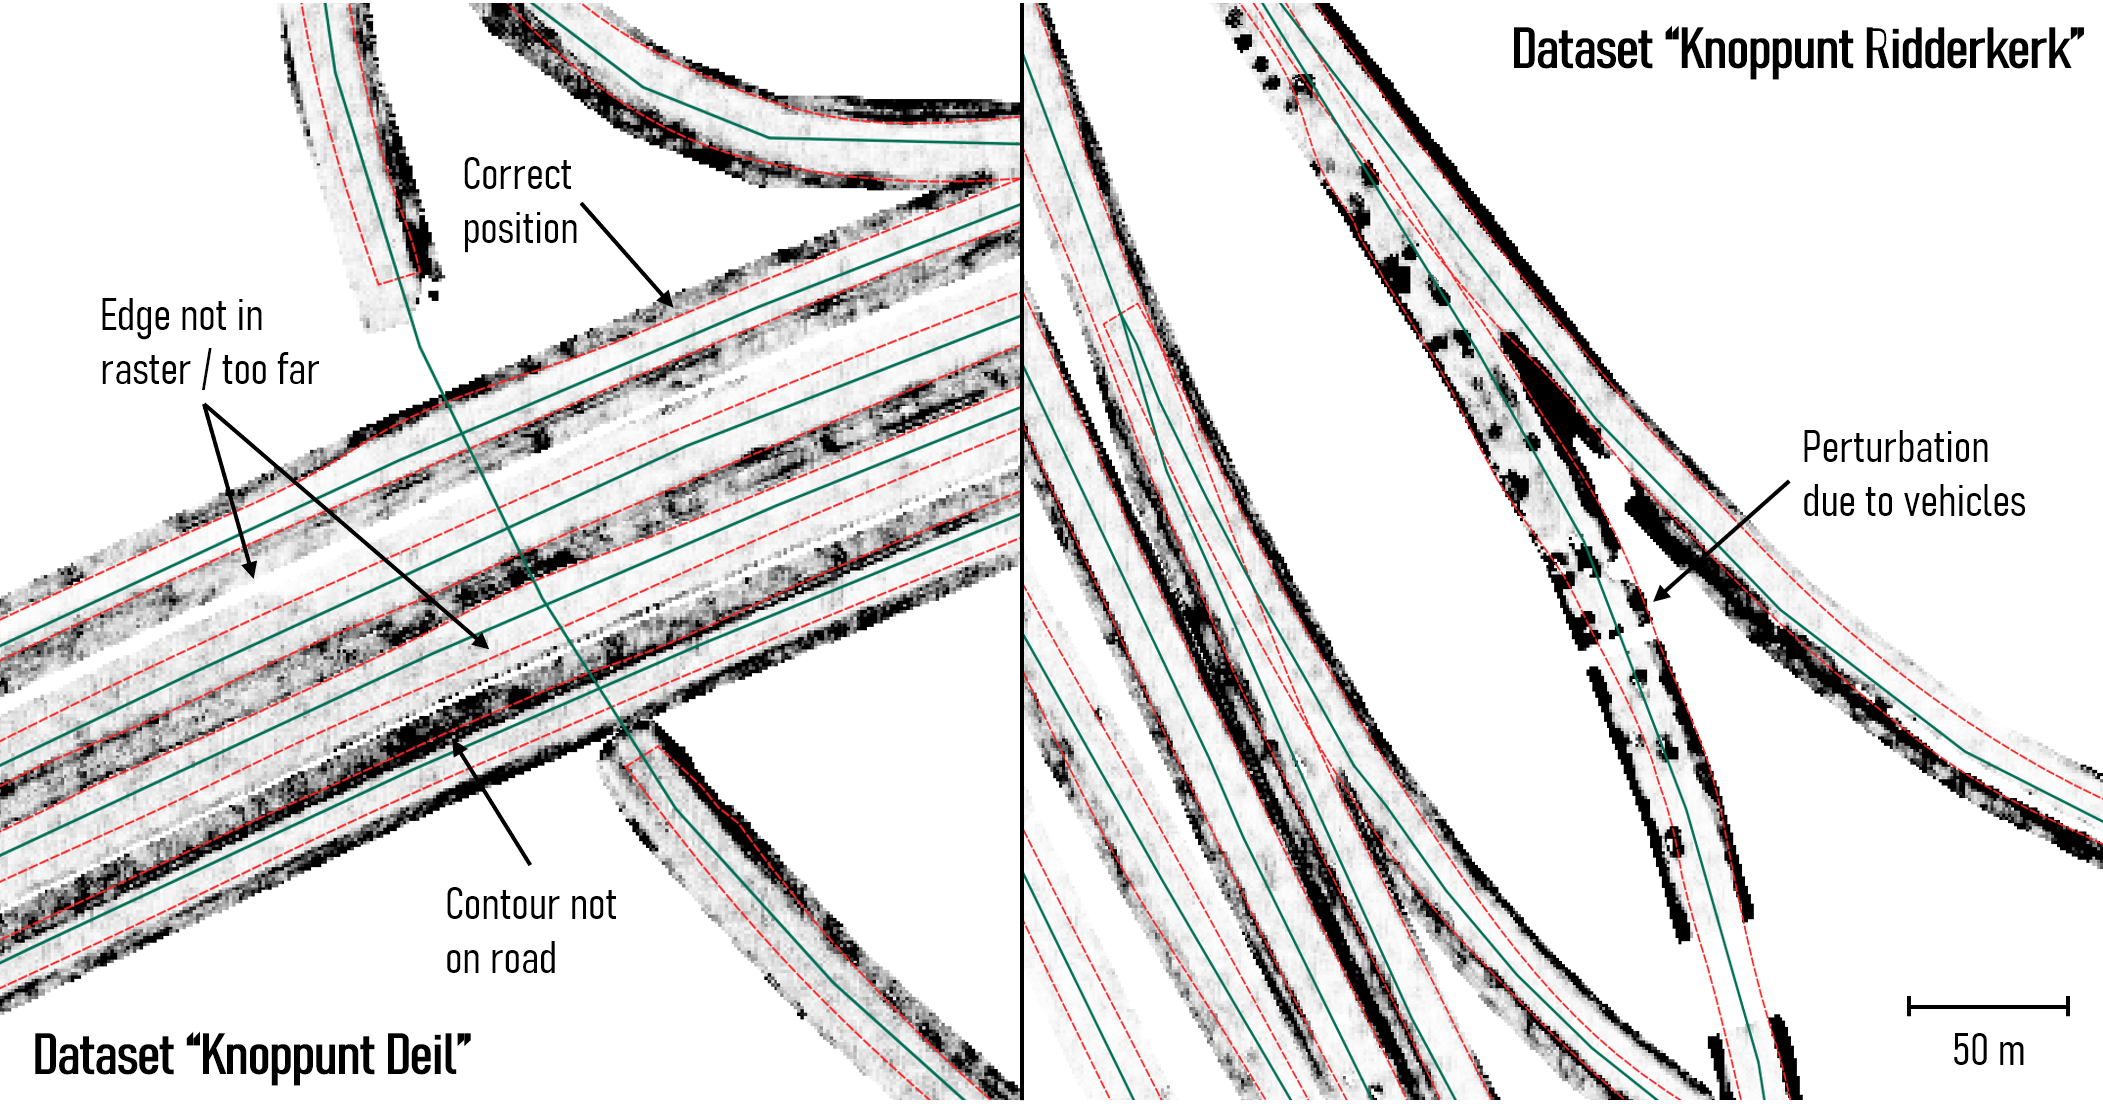
\includegraphics[width=\linewidth]{final_report/figs/activecontouroptimisation1.png}
    \caption{Visualisations comparing optimised edges to the underlying attractor maps.}
    \label{fig:activecontouroptimisation1}
\end{figure}

In terms of iterations, I decided to work solely with a maximum number of iterations (parameter \codeword{max_iterations}) rather than to use condition-based termination. Setting a condition would terminate the optimisation process when the contours no longer move significantly, i.e. it checks when a minimum displacement threshold first becomes violated. Where the attractor maps are perfectly suitable for active contour optimisation, this approach works well. However, letting the contours evolve in such a way where the attractor maps are sub-optimal results in the drastic enlargement of the generated artefacts, as well as an unacceptable increase in computational complexity. This happens, for instance, where edges are not defined well enough, and where Lidar gaps are present. I found iteration limits between 1000 and 5000 to be the most effective.

The time step parameter $\gamma$ and the number of pixels the contours are allowed to shift in a single iteration (parameter \codeword{max_px_move}) can be used to further fine-tune how quickly the optimisation lets the contours evolve. I set these two values to 0.005 and 1 respectively, which corresponds to a relatively slow iteration, appropriate to the small-scale changes we desire (generally, we wish to move the edges only by up to a few metres.

The above configuration of values is the result of a process of iterative combined revision of the values themselves, and the attractor map generation technique, as I mentioned in Section \ref{sub:m_activecontours}. While I experimented with a wide range of parametrisations, the possibility remains that a better one exists. The parameters themselves offer many permutations to try, and the fact that the preliminary edge and attractor map generation also affects the results only increases the range of possibilities.  

However, despite having tried most types of parameter configurations and many different adjustments to the preliminary edges and attractor maps, I was unable to find a configuration that produces satisfactory results within the development time reserved for this step. The quality of the optimised edges is simply not good enough to be used to classify Lidar points reliably based on them. The situation was made worse by the fact that the combined computational complexity of generating high-resolution attractor maps and of using the optimisation algorithm made the refinement procedure a rather difficult and time-consuming task. This is what lead to my decision to instead focus on improving the quality of the preliminary edges and use them directly in the \ac{tin} construction step. 

\subsubsection{Choice of algorithm}

Contributing to the above uncertainty regarding the effectiveness of active contour optimisation is the fact that in relevant literature (e.g. \cite{boyko_funkhauser_2011}), mentions of its ineffectiveness relative to more sophisticated algorithms is made. My hypothesis was that with a sufficiently good pre-selection of Lidar points and pre-processing of attractor maps, conventional active contour optimisation could still work well, but this appears not to be the case in practice.

Lesser known, but more sophisticated offshoots of active contour optimisation exist, but have no open-source Python implementations. One such example is the "ribbon snakes" method. Considering the volume of further tasks in this project, I opted not to attempt to implement it based on first principles, especially considering that their superiority is not clearly demonstrated in relevant literature. They, too, are prone to producing artefacts of various types, even if they perform slightly better than conventional active contour optimisation.

\subsubsection{Using the implementation}

The following lines of code may be used to run active contour optimisation and export the attractor maps and resulting optimised edges:

\begin{verbatim}
roads.optimise_edges(size = 0.5,
                     a = 0, b = 0.01, g = 0.005,
                     w_l = 0.05, w_e = 1,
                     max_iter = 1000)
roads.write_maps(fpath = maps_fpath)
roads.write_contours(fpath = conts_fpath)
\end{verbatim}

The first argument \codeword{size} in the active contour optimisation method corresponds to the desired pixel size. The rest of the parameters expose some of the active contour optimisation parameters that I found the be useful for making smaller changes to the algorithm's behaviour. The arguments \codeword{a}, \codeword{b} and \codeword{g} correspond to $\alpha$, $\beta$ and $\gamma$ respectively, while \codeword{w_l} and \codeword{w_e} correspond to the two parameters controlling attraction to brightness and edges (\codeword{w_line} \codeword{w_edge} respectively). The last parameter sets the maximum number of iterations.

The \codeword{.write_maps(maps_fpath)} method writes all attractor maps generated (one per \ac{nbrs} part) as GeoTIFF rasters, tagging the file name with the relevant \ac{nbrs} ID and part ID. Hence, the argument file name is expected to correspond to the first part of the file name only, e.g. \codeword{.../C_39CZ1_map} would work. Reserving a separate folder for these is recommended. The contours are written as a single Shapefile.

In the class, the maps can be found in the variable \codeword{.nbrs_maps[nbrs_id][part_id]}, while \codeword{.nbrs_contours} contains the contours in the form of a GeoDataFrame.

\subsection{TIN construction}
\label{sub:r_tinconstruction}

\begin{figure}
    \centering
    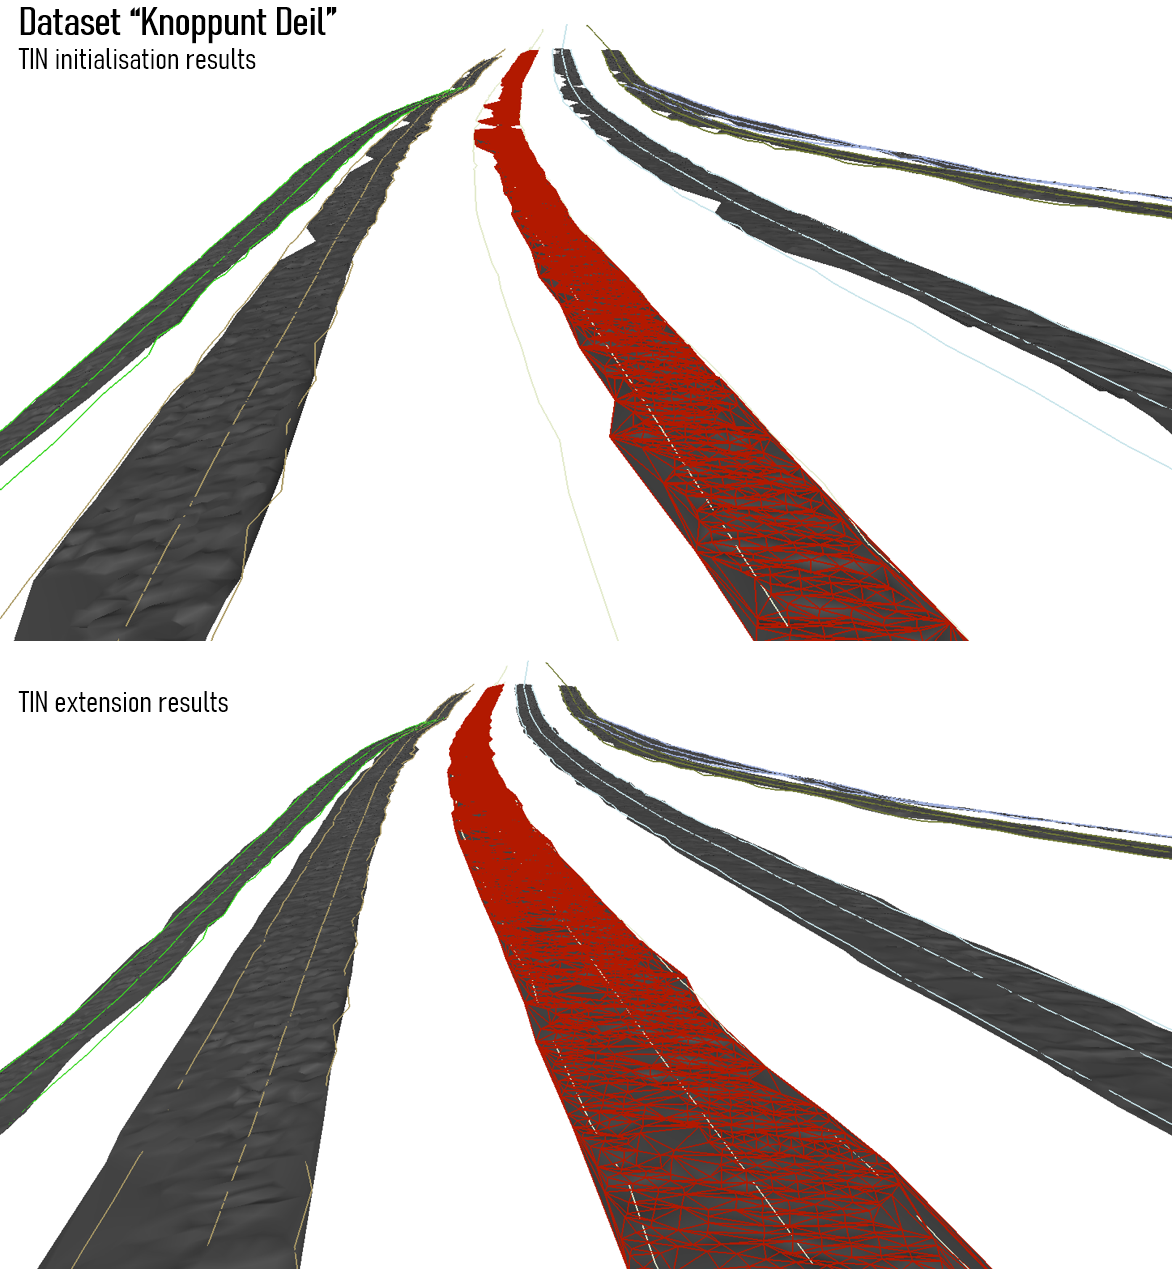
\includegraphics[width=\linewidth]{final_report/figs/tinconstruction0.png}
    \caption{Visualisations illustrating the results of \ac{tin} initialisation and extension.}
    \label{fig:tinconstruction0}
\end{figure}

By adjusting my methods to the circumstance of not being able to produce accurate enough optimised edges, I created a different implementation than originally planned, but one which is still robust and accurate. Figures \ref{fig:tinconstruction0} and \ref{fig:tinconstruction1} show examples of the resulting models compared with the preliminary edges and preliminary elevations. The images in Figure \ref{fig:tinconstruction0} show an initial \ac{tin} surface, and the same \ac{tin} after the extension stage. In these figures, the preliminary edges are shown because the initial \ac{tin} surface is seeded halfway between them, and because the \ac{tin} is only allowed to grow between them in the initialisation stage. The upper, large-scale image in Figure \ref{fig:tinconstruction1} shows and overview of all \ac{tin} surfaces in the \textit{Knooppunt Deil} dataset, and the bottom two images show small-scale examples of typical extension artefacts. The \ac{tin} structure is highlighted in one of the \ac{tin}s in Figure \ref{fig:tinconstruction0}.

\subsubsection{TIN initialisation}

A comparison of the initialisation step's insertion boundary is shown in Figure \ref{fig:tinconstruction0} both with initial \ac{tin}s and extended ones. The pre-selection step takes place in 2D, but for viewing convenience I used preliminary edges in this example visualisation, which are originally 3D geometries (in contrast with the optimised edges, which are 2D geometries).

While in most cases this does not represent an practical issue, my results suggest that there is a theoretical limitation to my methods. Since they were inspired by ground filtering algorithms, they are not particularly sensitive to gradual changes in the road surface, and especially insensitive to smooth transitions. The approach appears to excel at eliminating outlier points that were left undetected during previous steps, and detecting the edges of the roads where they are clearly defined by a significant vertical shift in the Lidar points, for instance a high curb or a wall. However, the conditional insertion tests often have difficulty in reliably recognising points close to, but not quite on the road surface where the edges are not well defined. Avoiding the insertion of such transitional points is key, because they may then act as a bridge between road points and off-road points in subsequent iterations, thereby allowing the surface to grow in undesired directions.

The image on the bottom left in Figure \ref{fig:tinconstruction1} shows an area that exhibits the above type of challenging scenario and causes a small region of sloping terrain points to be added to the initial \ac{tin}. The bottom right image in the same figure shows a similar type of artefact which occurs due to \ac{nwb} getting as close as within 5-20 centimetres from the outer edges of the bending road, resulting in the insertion of many off-road points. In the latter case, it is possible that the "bridge" points were already inserted in the seeding step, because the outer preliminary edge was constructed far beyond the road's real edge.

Had my original intention of producing more accurate (optimised) road edges succeeded, this would not have been a problem because the pre-selected Lidar points would have nearly all part of the road surface. Although I adapted my approach to the less optimal quality of the input edges, I was unable to completely overcome this limitation without a complete redesign, which was not possible within the available timeframe. Fortunately, in practice the initial \ac{tin} models are almost always well-behaved around the centrelines, and suffer from very few artefacts of this kind where \ac{nwb} is correctly positioned. The careful conditional insertions when growing the \ac{tin}s (where not only one, but multiple surrounding triangles are used to model the planar trend in the surroundings) helped mitigate this issue significantly.

For the \ac{tin} initialisation step, I used an elevation discrepancy threshold of 10 centimetres, and an angle threshold of 0.12 radians (about 7 degrees) in my final configuration. For the radial point queries that occur at the locations of successful insertions (to fill the buffer for the next iteration), I used a radius of 1 metre.

In all study areas, and especially where \ac{nwb} lies correctly on the road surface in 2D, my approach produces smooth 3D surfaces in which, as Figure \ref{fig:tinconstruction0} shows, most of the variation is solely due to noise in the Lidar data. Off-road points are only inserted in significant numbers, where the above conditions are satisfied; i.e. a smooth transition characterises the edge of the road or the underlying preliminary or optimised road edges were also significantly shifted outside of the road surface due to problems with \ac{nwb}.

\subsubsection{TIN extension}

Figure \ref{fig:tinconstruction0} shows the visual appearance of one particular \ac{nbrs} part before and after applying \ac{tin} extension, in a location where it works nearly perfectly. The effectiveness of this step relative to its planned purpose is not uniform across all areas. Most road geometries allow it to perform well, but in certain places it may only serve to further exaggerate pre-existing artefacts.

\ac{tin} extension considers additional "rings" of points progressing away from the road's centre and moving towards the edges - even beyond them, if desired. For the final results I used 5 steps, each extending the boundary by half a metre via buffering, and subtracting it from the polygon formed by the previous boundary to obtain the ring-shaped region of interest. Only those points are considered for insertion, which fall into the given region of interest in each iteration. The first iteration starts at a boundary half a metre from the seed geometry, hence 5 steps of 0.5-metres each expand the maximum distance from the centre to 3 metres, meaning that the largest boundary will be 6 metres from the centre of the road. One may notice that this is still smaller than the maximum road width I allowed in the preliminary edge approximation step (7 metres). There are two reasons for this; firstly, in my final results I primarily used \ac{tin} extension to extend initial \ac{tin} surfaces \textit{within} the width of the preliminary edges. Secondly, wherever the width of the preliminary edges goes below the maximum (which happens quite often), this still represents an extension beyond those boundaries.

For instance, consider the example shown in Figure \ref{fig:tinconstruction0}. In the highlighted initial \ac{tin}, the width of the model is only about 3 to 5 metres on average, even though the preliminary edges are 6 to 7 metres apart on average (close to the allowed maximum), not all points between them were inserted into the \ac{tin} in the "first pass" provided by \ac{tin} initialisation. \ac{tin} extension can solve this issue, effectively by executing additional passes over the candidate points.

In the same visualisations, the road on the left of the highlighted one has a slightly thinner representation in the preliminary edges, which are already mostly filled by the \ac{tin} during the initialisation stage. For this particular road, extending beyond the preliminary edges is more important than reconsidering data within the preliminary edges. In this specific case, it is the hard shoulder that gets added to the \ac{tin} during extension.

Since the extension procedure considers points beyond the preliminary or optimised edges, it needs to exercise caution against including off-road points. In places where the edges underestimated the road width, further surface points may be discovered and added to the model - which is the main purpose of this step. However, where the edges are correct, it is important that the algorithm does not add further points. The same goes for areas affected by the artefacts described in connection with the bottom two visualisations in Figure \ref{fig:tinconstruction1}; i.e. \ac{tin} extension should try not to worsen them.

Therefore, the algorithm uses stricter thresholds for the conditional insertions than the \ac{tin} initialisation step. In my final configuration, the values are 3 centimetres for the elevation discrepancy threshold (elevation above underlying triangle), and 0.04 radians (about 2 degrees) for the angle threshold. The radius of the buffer-filling queries was also reduced to 0.8 metres.

While such a conservative parametrisation certainly avoids the addition of clearly defined outliers, I found it to offer only a partial solution to the above issues. After some careful inspection, I concluded that in almost all cases, pre-existing "bridge points" from the \ac{tin} initialisation step appear to be the culprits. They eliminate the gradients that would otherwise stop the extension from growing in a particular direction. Furthermore, it appears that the transition from road to off-road surfaces may occasionally take place on such a fine scale that not even these thresholds can prevent the surface growing towards them, even where \ac{tin} initialisation did not introduce such bridges.

\begin{figure}[h]
    \centering
    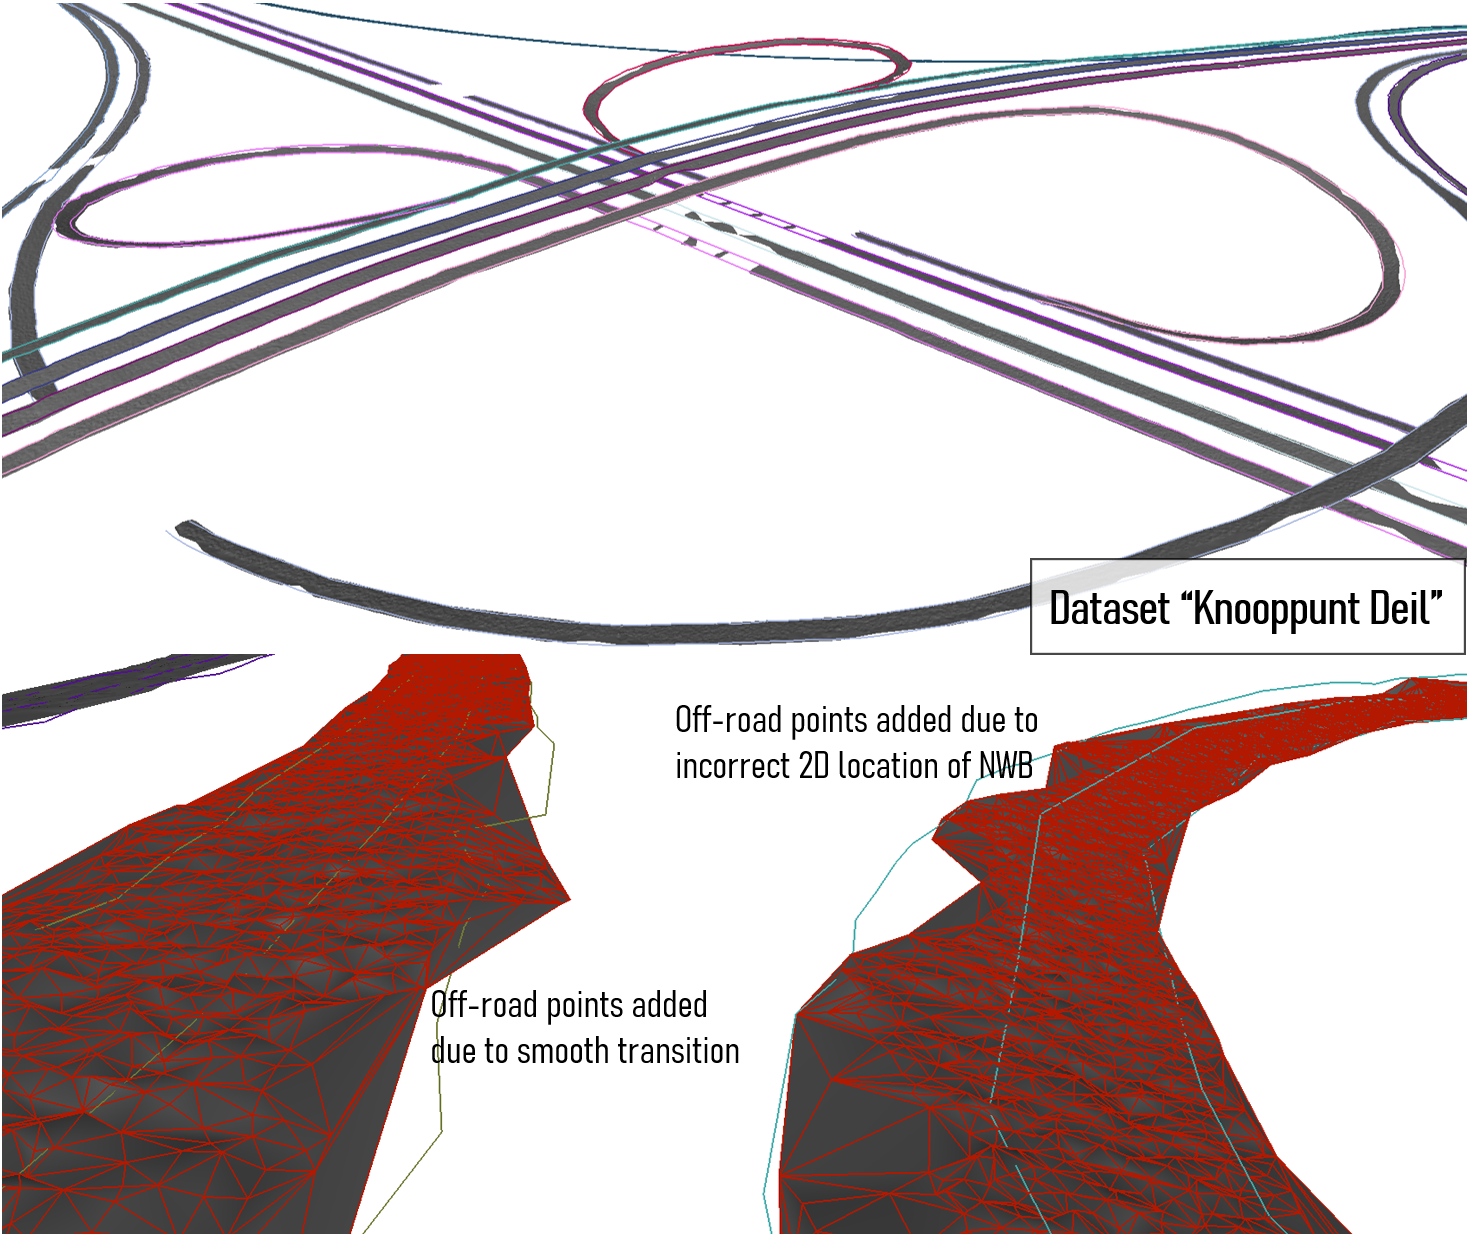
\includegraphics[width=0.9\linewidth]{final_report/figs/tinconstruction1.png}
    \caption{Visualisations providing an overview of constructed \ac{tin}s and illustrating \ac{tin} artefacts.}
    \label{fig:tinconstruction1}
\end{figure}

\subsubsection{On using small thresholds}

An obvious solution would then be to use preliminary edges that are close to the roads' centrelines, and to make the parametrisation of both \ac{tin} initialisation and \ac{tin} extension even stricter. However, there is a specific reason why this approach is guaranteed to fail: both parametrisations are already lower than \ac{ahn3}'s vertical accuracy. As \ref{sub:ahn} mentions, \ac{ahn3} has an elevation uncertainty of 15 centimetres at 95\% uncertainty. This means that many insertions will actually fail due to the noise, not because of real-life features.

The parametrisation of \ac{tin} initialisation (10 centimetres for elevation/distance tests, 7 degrees for the angles) is already on a scale that falls within the territory of random noise. However, since the radial buffer-filling queries fetch many points rather than just a single neighbour, this generally does not affect the effectiveness of the method; the algorithm will inspect enough neighbours to still find at least a few that are conformant, despite the noise. Even where this fails to an extent, the \ac{tin} extension algorithm will provide the additional passes that are necessary to overcome the issue; this is precisely what happened with the highlighted road in Figure \ref{fig:tinconstruction0}.

As a result of this phenomenon, reducing the thresholds any further without increasing the query radius will inevitably block the surface from spreading into certain areas. Increasing the query radius is, in turn, not desired because it will create too large buffers (increasing computational complexity drastically), and cause large triangles to be constructed in the \ac{tin}, which can in turn act as blocking factors in their own right, if they do not represent the trend of the points in their interior accurately. Using large query radii also increases the chances of spreading the \ac{tin} off the road surfaces, as it will result in more off-road points getting added to the buffers.

In \ac{tin} extension, I could use smaller thresholds than during initialisation because of the differences in the underlying workflow. Since extension considers "layers" of points progressing away from the centres of the road, it considers candidate points in a more "orderly" fashion. In \ac{tin} initialisation, the \ac{tin} only grows towards a certain area if insertions lead the algorithm there, whereas the repeated seeding mechanism in the extension stage represents a more \textit{targeted} growing approach. In practice, this means that the candidates are simply examined in a better order, leading to more efficient decision-making. This counteracts the increased impact the Lidar noise has on the scale of the thresholds that are being used.

A side-effect of this is that growing may be restarted during extension after a relatively large hiatus, leading to large triangles appearing in the \ac{tin}s. The hiatuses - or more precisely, the failed insertions in them - are mostly caused by the larger, slightly inaccurate triangles which I already mentioned in the previous paragraph. This can be seen in the \ac{tin} structure in the top image in Figure \ref{fig:tinconstruction0} - while the right half of the suspected area of the road has points spaced uniformly, the left side has large, slightly inaccurate triangles that prevented Lidar points from being inserted within their areas and growing the \ac{tin} further in that direction. As the bottom image in the same figure shows, the "second pass" over the data via the \ac{tin} extension solved this issue for the most part, although some of the large triangles remained.

Inspecting a larger area around the point that is being considered for insertion (instead of just the one triangle containing it) could reduce the impact of this issue, but it is costly in terms of computational complexity. This is part of the reason why I only use that approach when inserting points in triangles touching the insertion boundary.

\subsubsection{Note on figures}

Both figures in this section (\ref{fig:tinconstruction0} and \ref{fig:tinconstruction1}) show \ac{tin} road surfaces that appear to be constrained by "invisible" external line geometries, as one would expect large triangles to fill the rest of the convex hull of the vertices in the Delaunay triangulation. Originally, I planned to use a \ac{cdt} to achieve this appearance, but in my final implementation I merely improved the appearance of the models before visualising them by removing meaningless triangles based on area and circumference thresholds. This proved to be effective in eliminating the large triangles and sliver triangles that appear in the \ac{dt} to fill the convex hull of the inserted points.

While these redundant triangles represent no issue in terms of interpolating elevations for \ac{nwb}, they make the visual interpretation of the results difficult. Exporting the \ac{tin}s after generating them automatically applies this filtering step in the final release of my code.

In this context, it is also important to point out that while \ac{ahn3} data gaps that are patched in with \ac{dtb} data are always completely covered by triangles in the \ac{tin}s if the preliminary edges extend through the gap. The reason why in the top image in Figure \ref{fig:tinconstruction1} this appears not to be the case, is that some of these triangles were large enough to be filtered out to improve visual appearance. The thresholds can be adjusted in my code to alter this behaviour.

\subsubsection{TIN point density}

While using 50\% of the \ac{ahn3} point density (via a thinning factor of 2) offered practical benefits for all pipeline steps up to this point (especially the Lidar segmentation and edge approximation steps), the \textit{quality} of the generated \ac{tin}s does not significantly increase as a factor of point density.

Before running the \ac{tin} construction procedure, the program is equipped with subclouds, each with Lidar points relevant to a specific \ac{nbrs} part. Since all prior steps are configured to keep as many of the surface points as possible, it is generally the case that their point density on the road surface is comparable to the thinned point density of the imported \ac{ahn3} data. Inserting such a large volume of points into the \ac{tin} may not always be practical. For instance, visualising the generated surfaces becomes slow even with modern software, and the stochastic Lidar noise becomes clearly visible (the ripples can be seen very clearly in Figures \ref{fig:tinconstruction0} \ref{fig:tinconstruction1} due to the 5-fold vertical exaggeration). This much detail may also be impractical for applications that deal with modelling processes on the surface itself, and has implications for the accuracy assessment (see Section \ref{sec:accuracy}).

The performance of this step thus depends on the input Lidar thinning. In practice, a thinning factor of 2 means that we are still working with around 10-30 Lidar points per m\textsuperscript{2}, which results in mediocre performance. While my implementation did take performance considerations into account initially (for instance the buffer-filling approach is the result of this), later modifications, such as working with multiple triangles and plane fitting when growing the road surface, resulted in the performance of the final implementation decreasing gradually. In particular, not running \ac{tin} extension can improve runtimes drastically, which may be useful for users who are only interested in interpolating \ac{nwb} elevations.

As I will further explain in Section \ref{sec:accuracy}), the system design guarantees that \ac{nwb} will generally lie on the \ac{tin} models in 2D, making it possible to interpolate elevations in it for its vertices. Exceptions to this rule occur in places where preliminary edge estimates or optimised edges disagree with \ac{nwb} badly. Where this occurs, \ac{tin} initialisation will not be able to insert points in the \ac{tin}s at the 2D location of \ac{nwb}. With preliminary edges, this may only occur where cross-sections were skipped too many times in a row where the road is not straight, which may happen in various circumstances I have already described in Section \ref{sub:r_edgeapproximation}. With active contour optimisation, this may occur more frequently, depending on the local density of generated artefacts.

\subsubsection{Two different kinds of quality}

While the above discussion focuses on describing issues with the quality of the generated \ac{tin}s, many of these issues are constrained to the academic goals of the project only. The academic goal related to the \ac{tin}s is to make them complete and accurate representations of the real-life road surfaces. This is the quality on which I primarily focused in this section, while the next section will see more mentions of quality in terms of their suitability for interpolating elevations for \ac{nwb}.

These two qualities need to be distinguished not only because of the conceptual differences, but because there are much less issues with the less academic goal of converting \ac{nwb} to 3D than with producing ideal road surface models. The reason is, that for the 3D conversion to be accurate, one only needs complete and accurate \ac{tin} surfaces close to where the centrelines are found in 2D. Fortunately, these locations generally correspond to areas which are less difficult to reconstruct accurately in 3D, than for instance the immediate vicinity of road edges.

\subsubsection{Using the implementation}

The following two commands may be used to run \ac{tin} construction and export the resulting 3D surface models:

\begin{verbatim}
roads.build_tin(max_dh_int = 0.1, max_angle_int = 0.12, r_int = 1,
                max_dh_ext = 0.03, max_angle_ext = 0.04, r_ext = 0.8,
                ext_steps = 5, ext_dist = 0.5,
                type_edges = 'preliminary')
roads.write_tins(fpath = tin_fpath)
\end{verbatim}

The first method invocation performs the \ac{tin} construction itself. The first line of arguments corresponds to the elevation and angle thresholds, and the buffer-filling query radius used in \ac{tin} initialisation, respectively. The role of the second line of arguments is identical, with the exception that they are used for \ac{tin} extension. The next two arguments (\codeword{ext_steps} and \codeword{ext_dist}) specify the number of extension steps to be performed, and the distance by which the query region should be expanded in each step. The first insertion boundary for extension is always a polygon created by buffering the seed LineString by 0.5 metres; the extension starts from this base boundary. If no extension is desired, \codeword{ext_steps} should be set to 0. The last parameter, \codeword{type_edges} can be set either to \codeword{preliminary} or \codeword{optimised}; it controls which type of road edges the user desires to use.

The second method invocation writes the \ac{tin}s to disk, one OBJ file for each \ac{nbrs} part As mentioned above, it also filters out large triangles and sliver triangles in the process. The supplied file path should only include the first part of the file name, as the \ac{nbrs} ID, part ID and file extension will be added automatically (for instance \codeword{.../C_39CZ1_tin} would work. Using a dedicated folder is recommended.

\subsection{Interpolation in TIN and snapping}
\label{sub:r_interpolation}

\begin{figure}
    \centering
    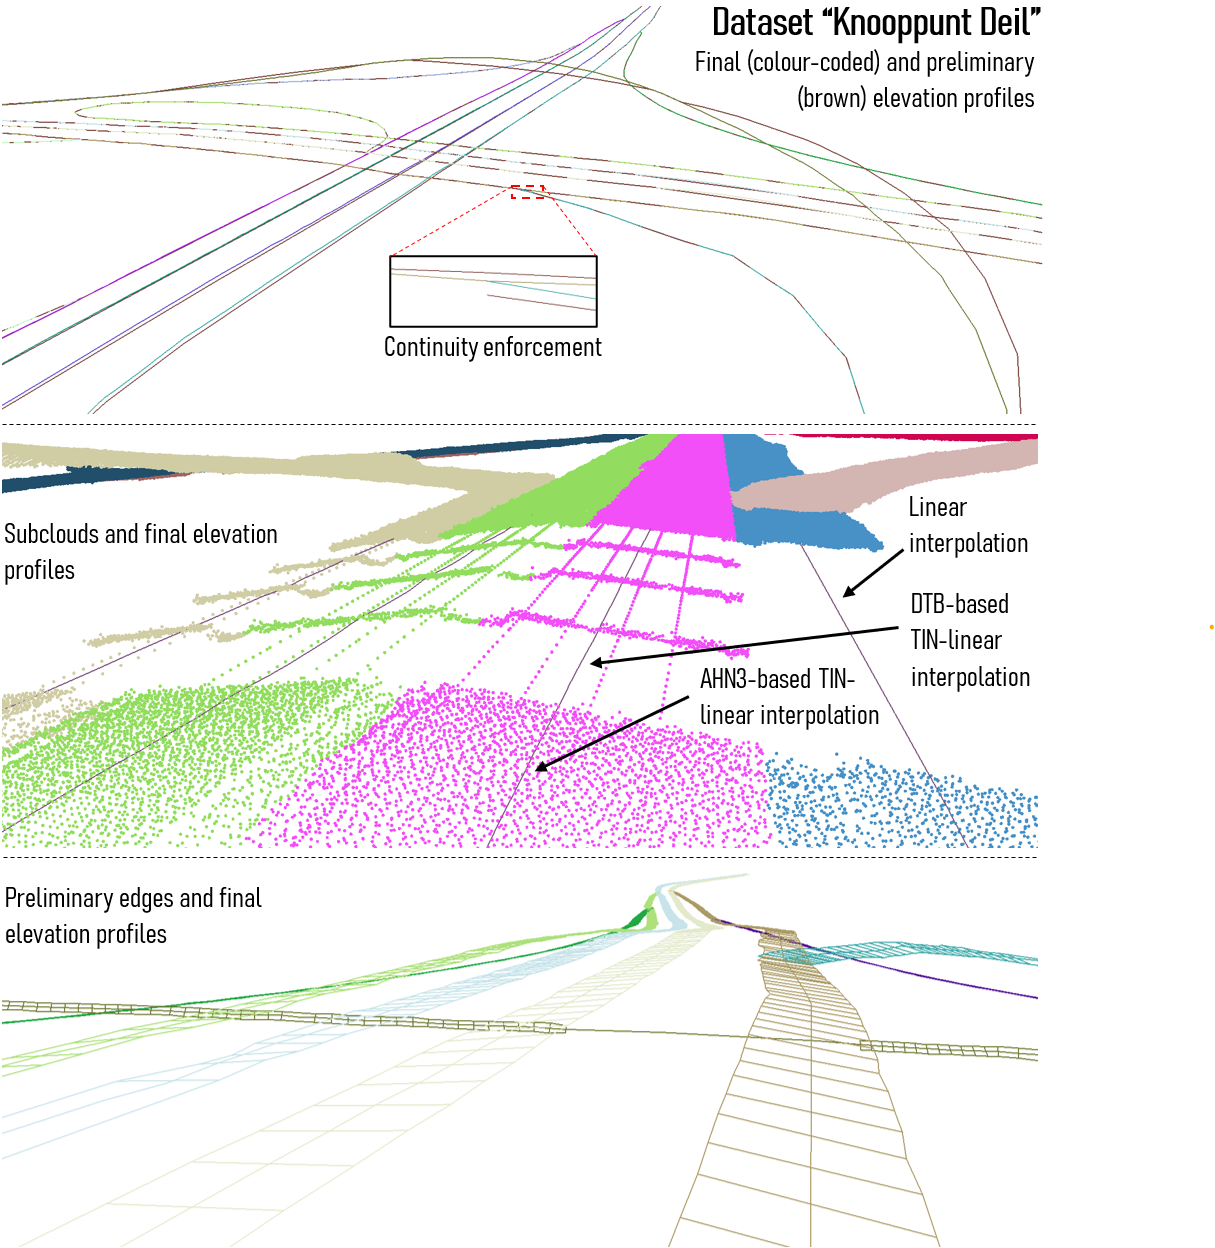
\includegraphics[width=\linewidth]{final_report/figs/elevationinterpolation0.png}
    \caption{Visualisations comparing final 3D conversion results to preliminary conversion, subclouds, and preliminary edges.}
    \label{fig:elevationinterpolation0}
\end{figure}

Figures \ref{fig:elevationinterpolation0} and \ref{fig:elevationinterpolation1} show examples of the results of interpolating elevations for \ac{nwb} in the \ac{tin}s generated in the previous step (including the use of the snapping feature that enforces continuity)). Visual inspection of the results reveals that the methods used to generate them are robust and effective under almost all circumstances, including where complex 3D relationships and the extensive presence of other types of occlusion are encountered. The example visualisations shown here contain comparisons between the final elevation profiles and various intermediate results, namely the preliminary elevations, subclouds and preliminary edges in Figure \ref{fig:elevationinterpolation0}, and the \ac{tin} models in Figure \ref{fig:elevationinterpolation1}).

Generally, the results are in line with my expectations both in terms of overall completeness and quality. I do not attempt to characterise the accuracy of the results in this section, for a quantitative (rather than qualitative) analysis, please refer to \ref{sec:accuracy}.

\subsubsection{Comparison with preliminary elevations}

Comparing the final 3D-NWB results with the preliminary elevations sheds some light on the nature of the improvements that are the result of the complex processing steps that occur in the later stages of the pipeline. The preliminary elevations (shown in a brown colour in the top visualisation Figure \ref{fig:elevationinterpolation0}) represent the 3D conversion that can be achieved using only a few simple steps of processing: \ac{nbrs} generation, elevation estimation, and the polynomial-based refinement step. The final results are coloured randomly based on their \ac{nbrs} IDs.

The first difference that stands out is that those \ac{nbrs} that I described as having complex vertical curvature and being difficult to model by polynomials in Section \ref{sub:r_elevationestimation} are modelled much more realistically in the final output. One only needs to take a look at the comparison in the top image in Figure \ref{fig:elevationinterpolation0}) to tell that it must be the final results that are correct, not the preliminary ones. The change represents a fundamental difference between these two stages in the pipeline. Preliminary elevation estimation has to rely on a workflow to detect elevation estimates corrupted by occluding geometry and to supply replacement values for them, while the final elevations come from \ac{tin} models that are guaranteed to only contain vertices that represent measurements of the relevant road's elevation.

While the biggest differences can be observed where the polynomial fits were poor in the preliminary elevation estimation stage, there are many other scenarios where smaller improvements can be seen. For instance, the preliminary elevations may contain outliers that were not detected as outliers in the refinement step. For instance on bridges, \ac{ahn3} may contain reflections from vehicles. These are often not far enough from the road surface to be replaced by polynomial values, introducting small spikes into the elevation series. In the final results, such outlier points are guaranteed not be be inserted into the \ac{tin} models, and cannot affect the 3D conversion as a result. The inset in the figure also illustrates that while while preliminary 3D conversion is not continuous across intersections, the snapping workflow ensures that the final 3D conversion is.

Another scenario in which clear benefits can be observed (not shown on these figures) is the presence of many occluded regions concentrated into a small area, or equivalently, one long occluded zone. In preliminary elevation estimation, such occluding features may attract the polynomial towards themselves, thus corrupting the fit and potentially introducing incorrect elevations into the profiles. This may happen, for instance, where many bridges are constructed across a motorway in a row, and the \ac{nbrs} is not long enough to include enough non-occluded elevation measurements. Later pipeline steps almost always recognise these mistakes for what they are (data gaps), and either use \ac{dtb} if available, or break the \ac{nbrs} into parts locally.

There are features in the final output that may be interpreted as a deterioration in quality with respect to the preliminary elevations, at least visually. Firstly, small jumps in elevation may be observed where \ac{ahn3} gives way to \ac{dtb} points the underlying \ac{tin}s. The new baseline elevation continues across the region where \ac{dtb} was used, and reverts to the \ac{ahn3}-based baseline elevation once the road emerges from the zone not covered by \ac{ahn3}. This is simply due to the temporal discrepancy between \ac{dtb} and \ac{ahn3}; using better support data would eliminate these shifts from the output. This is only visible in the middle image in Figure \ref{fig:elevationinterpolation0}, and the reader is referred to Figure \ref{fig:lidarsegmentation1} and Sections \ref{sec:accuracy} and \ref{sec:r_comparison} for further details.

Lastly, one may observe that the amount of small-scale noise in the final 3D-NWB output is noticeably larger than that in the preliminary profiles. This also has a simple explanation: the preliminary elevations are based on taking the median of the elevations of a small patch of Lidar points, whereas the final elevations are all based on 3 samples each, due to having used \ac{tin}-linear interpolation. The amount of noise is thus no greater than the stochastic scatter in \ac{ahn3}; it is only visible in the visualisation due to the vertical exaggeration.

\subsubsection{Comparison with subclouds}

This comparison is demonstrated in the middle image in Figure \ref{fig:elevationinterpolation0}. The most important aspect here is that the final 3D road centrelines all lie flat on those parts of the Lidar subclouds, which one intuitively recognises as road surfaces. This is always the case as long as \ac{nwb} is correctly positioned, such as in this location.

The figure shows that this also holds for regions affected by occlusion. In places where \ac{dtb} was added to the subcloud in the Lidar segmentation step, the centrelines are shifted vertically to conform with the surfaces defined by \ac{dtb}. Where \ac{ahn3} coverage reappears, they immediately shift back to its elevation, creating a geometry akin to suspension bridges in this example visualisation. Regardless of which dataset is used, the main point here is that the 3D conversion continues across the gaps without snapping to the bridges above that are causing the periodic occlusion.

The visualisation also illustrates that linear interpolation through regions with no measurements represents a good solution for small gaps of coverage where roads are straight. The road with the blue-coloured subcloud (on the right) has no \ac{dtb} coverage, hence the small patches of \ac{ahn3} points between the bridges could also not be detected. In spite of this, the elevations are actually more optimal here than elsewhere, because they are not affected by the small sifts introduced by \ac{dtb}.

\subsubsection{Comparison with preliminary edges}

This comparison reveals the interestingly, the final 3D conversion of the centrelines and the preliminary edges are in near-perfect agreement with each other where coverage is good. As the bottom image in Figure \ref{fig:elevationinterpolation0} shows, even a five-fold vertical exaggeration cannot reveal significant differences between them. This is interesting, as there are various pipeline steps in-between the generation of these results; most importantly, \ac{tin} generation. Small differences are only found between the elevations of the preliminary edges and 3D-NWB, where the preliminary edges were generated off the road surface, in which case the final results represent the correct elevation.

While the two outputs are not directly comparable, the exceptionally good match between them indicates that a 3D conversion with similar quality could potentially be achieved via a procedure that involves the subclouds and 2D centrelines only, perhaps using a workflow based to some extent on that which currently I used to generate the preliminary edges.

It is also important to note here that while the preliminary edges may be missing vertices in some places (indicated by the cross-sections also being absent), this is not the case in any of my final 3D-NWB results. As long as the centreline is found between the edges, a \ac{tin} will be constructed locally and \ac{tin}-based elevations will be computed. As I already described previously, this is only violated in places where many cross-sections are skipped in a row, which is rare in my results.

\begin{figure}[h]
    \centering
    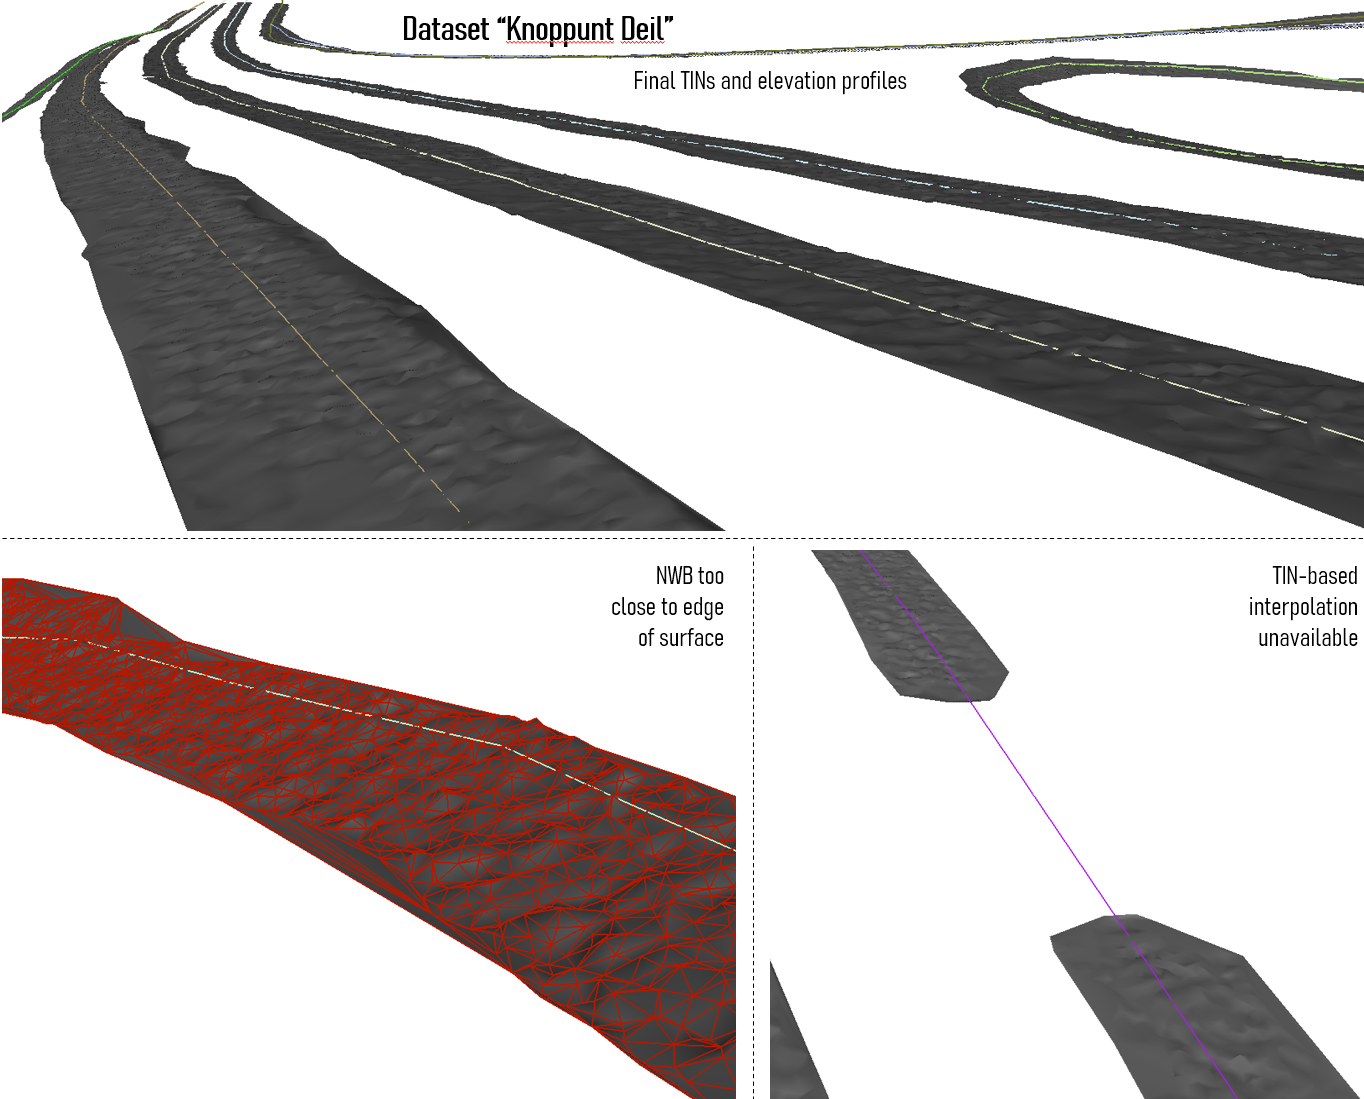
\includegraphics[width=0.9\linewidth]{final_report/figs/elevationinterpolation1.png}
    \caption{Visualisations comparing final 3D conversion results to the underlying \ac{tin} models.}
    \label{fig:elevationinterpolation1}
\end{figure}

\subsubsection{Comparison with TIN models}

Example comparisons between the final output and the \ac{tin}s are shown in Figure \ref{fig:elevationinterpolation1}. An interesting aspect of this comparison is that the final 3D-converted centrelines are often found slightly above or below the model (less than a centimetre, typically). This is best evidenced in the output by the intermittent disappearance of the 3D centrelines beneath the \ac{tin} triangles. This is the result of the georeferencing of \ac{nwb} being coarse \textit{relative to the \ac{tin}s} even after applying vertex densification. \ac{nbrs} parts only have vertices approximately every 5 metres, whereas \ac{ahn3} has up to 10 to 30 points per m\textsuperscript{2} after after thinning using a factor of 2. This disparity simply indicates that if we wanted to, we could sample the \ac{tin} at smaller intervals to increase the output's vertical resolution. However, \ac{ndw} officially requires elevations only to be estimated at the original \ac{nwb} vertices, which can be several times further apart even than my densified vertices. In other words, these \ac{tin}s offer far more detail than that which would be minimally required for the conversion, as expected from such a high-resolution surface model.

An example where \ac{nwb} gets close to the edge of the \ac{tin} is shown in the bottom left image. This is representative of the typical severity of the \ac{nwb} georeferencing issue in sharp bends. While it was difficult to overcome numerous processing difficulties related to this problem with \ac{nwb}, it bears almost no influence on the effectiveness of the \ac{tin} interpolation process as long as the \ac{tin} exists locally. Where \ac{nwb} lines are close to road edges, the underlying \ac{tin} models will still always describe the surface of the road according to our expectations. They will potentially include off-road points, but from the point of view of the 3D conversion of \ac{nwb}, this does not matter. Even if \ac{nwb} is not on the road surface, the \ac{tin} will likely be constructed locally and off-road elevations will be interpolated for it.

The interpolated elevations will always correspond to \ac{nwb}'s exact horizontal position, meaning that as long as its georeferencing is not corrected, the interpolated elevations will also not correspond to the road's real centreline. This could mean a significant deviation if \ac{nwb} is not on the road surface, or even if it is on the road but the road's surface is somewhat tilted sideways. Rectifying \ac{nwb}'s georeferencing would automatically solve this, no modifications to the algorithms would be needed.

Where no \ac{ahn3} \textit{or} \ac{dtb} coverage is available, the \ac{tin} will not exist and values are interpolated linearly inside the elevation profiles. A location with this property is shown on the bottom right in Figure \ref{fig:elevationinterpolation1}. Such gaps correspond to zones \textit{between} \ac{nbrs} parts, hence the two \ac{tin}s shown in this image belong to two different \ac{nbrs} parts.

\subsubsection{Using the implementation}

The following two commands may be used to run the final elevation interpolation code, and export the resulting 3D-converted version of \ac{nwb} as a Shapefile:

\begin{verbatim}
roads.interpolate_elevations()
roads.write_all(fpath = accurateZ_fpath,
                to_drop = ['geometry_simpleZ'])
\end{verbatim}

The algorithm does not have a parametrisation, hence the method invocation does not require any arguments. The \codeword{.write_all()} invocation requires a list of GeoDataFrame columns to drop, as the Shapefile can only have one set of geometries in it. The column name in \codeword{['geometry_simpleZ']} corresponds to the preliminary elevation estimates. The original 2D \ac{nwb} geometries are always dropped automatically, so that column does not need to be manually specified.

In the \codeword{nbrs_manager} class, the final results are added to the class's \codeword{.nwb} variable, as the \codeword{geometry_simpleZ} geometry column of the GeoDataFrame. Since Shapefiles also cannot accept arrays into their attribute tables, the vertex origin indicators (AHN3/DTB/linear interpolation) are also not written into the output file. These can be found in \codeword{.wvk_z_origins[wvk_id]}, a dictionary that needs to be indexed with the \textit{wegvak}'s ID whose vertex origins are desired.

\section{Accuracy assessment}
\label{sec:accuracy}

In this section, I will present the accuracy assessment results focusing on a particular dataset: \textit{Knooppunt Deil}. This dataset exhibits most of the unique features that are relevant for this part of the analysis, and it is my hope that such a "case study" approach makes understanding the assessment's results more straightforward. Following the case study, I will present and discuss an overview of the relevant accuracy metrics for all testing datasets, in a tabulated format.

I will first focus on the results of computing local sampling densities and formal output accuracy values (error propagation results). Then, I will discuss how often the accuracy needs to be deemed unknown and for what reasons. Lastly, the completeness of the output \ac{tin}s relative to the \ac{bgt} reference polygons will be examined. Please refer to the relevant sections in Chapter \ref{chap:mm} (\ref{sub:accuracyoverview} and \ref{sec:m_accuracyassessment}) for the background theory and the detailed description regarding the assumptions I made.

\subsection{Empirical accuracy assessment}
\label{sub:accuracyempirical}

\begin{figure}
    \centering
    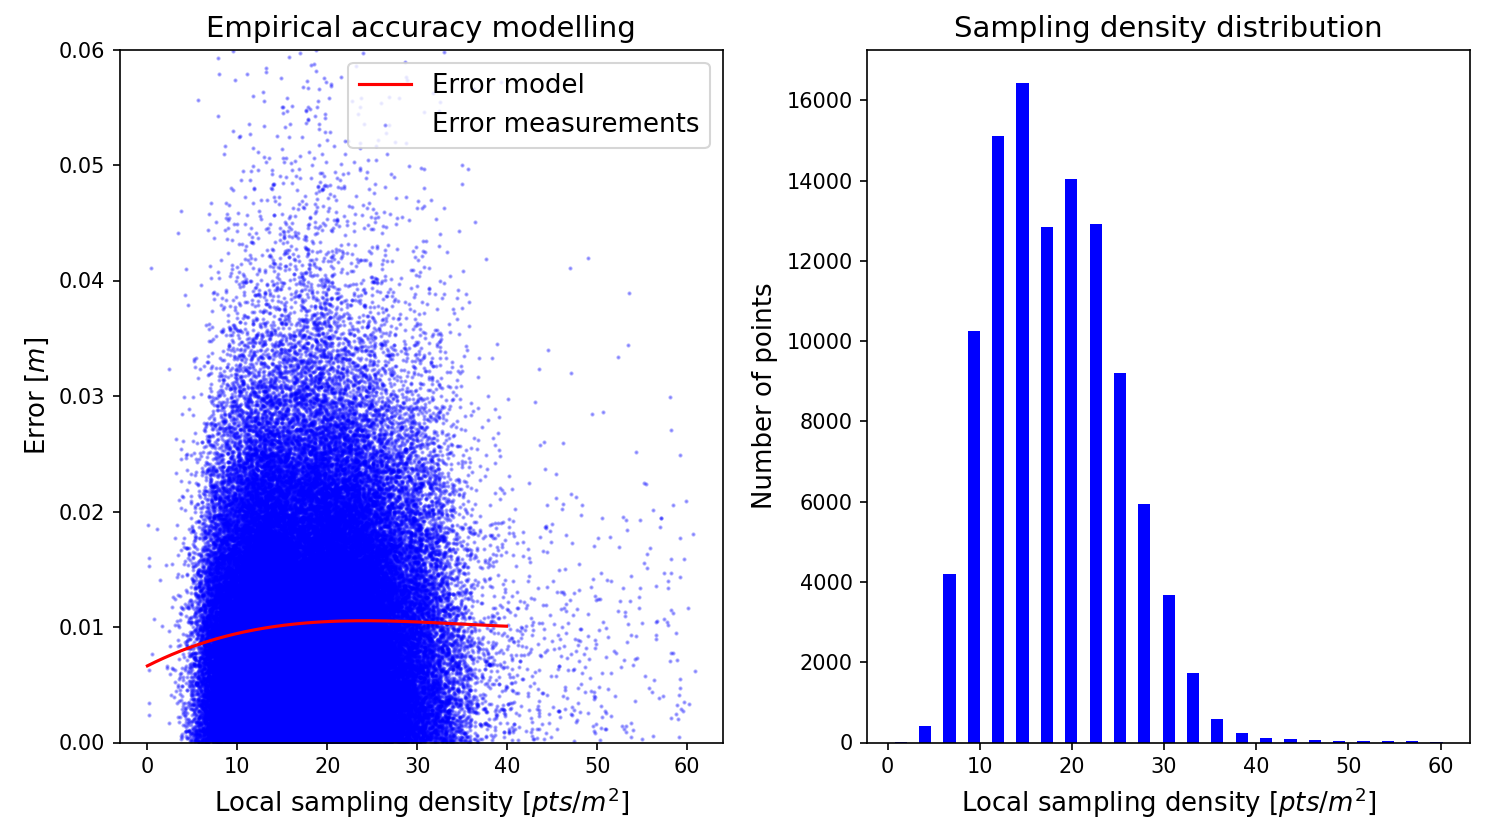
\includegraphics[width=\linewidth]{final_report/figs/empiricalaccuracy0.png}
    \caption{Charts demonstrating the outcome of the empirical accuracy assessment process.}
    \label{fig:empiricalaccuracy0}
\end{figure}

As I briefly mentioned in Section \ref{sub:accuracyoverview}, I first attempted to assess accuracy based on an empirical approach. Before performing the necessary steps, I was yet unaware of how the combination of factors that define output accuracy interact in our particular case. Most importantly, I was yet to discover that a range of assumptions regarding ground filtering accuracy, influence of surface ruggedness and sampling density can be made. In fact, it was this failed attempt that directed my attention to the fact that in our particular case, there are very few external factors that influence accuracy.

My initial hypothesis was that the primary influence on accuracy has to be sampling density and interpolation error, because ground filtering errors and surface ruggedness already appeared to me as irrelevant based on my experience with the data and the results. To be able to verify the hypothesis and compute empirical errors based on it, I constructed an error model and derived errors for each output vertex from it. I constructed the model by removing samples (vertices) from the output \ac{tin}s, interpolating their values via the \ac{tin}-linear method, and computing the differences between the removed Lidar samples, and the interpolated elevations (in essence, a jackknife approach). I fit a cubic polynomial on the part of the scatter where we have enough data, and derived \ac{nwb} accuracy values from it.

While I was doing this, I noticed that all my output errors were extremely small, and all roughly the same. This made me start suspecting the irrelevance of sampling density in our particular scenario, so I plotted the data and the model to verify this new hypothesis. Figure \ref{fig:empiricalaccuracy0} shows an example visualisation created from the empirical accuracy assessment of testing dataset \textit{Knooppunt Deil}. The chart on the left shows local sampling density plotted against the jackknife errors, computed for about 10\textsuperscript{5} \ac{tin} vertices (10\% of the total number of \ac{tin} vertices of all \ac{tin} models generated from this testing dataset).

While at a first glance one might think that the inverse parabola shape in the scatter plot represents a meaningful trend, it does not, in fact, possess the correct shape for the relationship. We know from literature that when a correlation exists between errors and sampling densities, it tends to be logarithmic, and the trend in my chart does not appear to have that property. The fitted model does appear to have a weak logarithmic component, but it shows errors to increase in the wrong direction (towards larger sampling density), and the predicted error magnitudes are far too small to be meaningful too. The histogram on the right reveals that the shape of the scatter plot does not correspond to a statistical trend that concerns a relationship between sampling density and jackknife error - it can be fully explained by the distribution of the sampling densities in the dataset.

What is also interesting in these plots, is that jackknife errors remain negligible even at the lowest values encountered. Overall, about 96\% of the jackknife samples showed an error less than 3 cm, which is well below the nominal vertical and horizontal accuracies of \ac{ahn3} and \ac{dtb}. In other words, we may safely conclude that the variation in jackknife accuracy, on the scale observed in this experiment can be explained simply by the noise in the input datasets. The random distribution of the variations, evidenced by the bell-shaped trend, further confirms this theory.

Although this analysis suggests that any errors in the output will be small and that they will be mostly independent of external factors, the qualitative and quantitative estimation of output accuracy is among the main goals of this project, hence I decided to find further evidence. This is why, even after performing the above analysis, I proceeded to propagate errors through the interpolation technique, and to also examine this in comparison with sampling density data.

\subsection{Formal accuracy assessment}
\label{sub:accuracyformal}

\begin{figure}
    \centering
    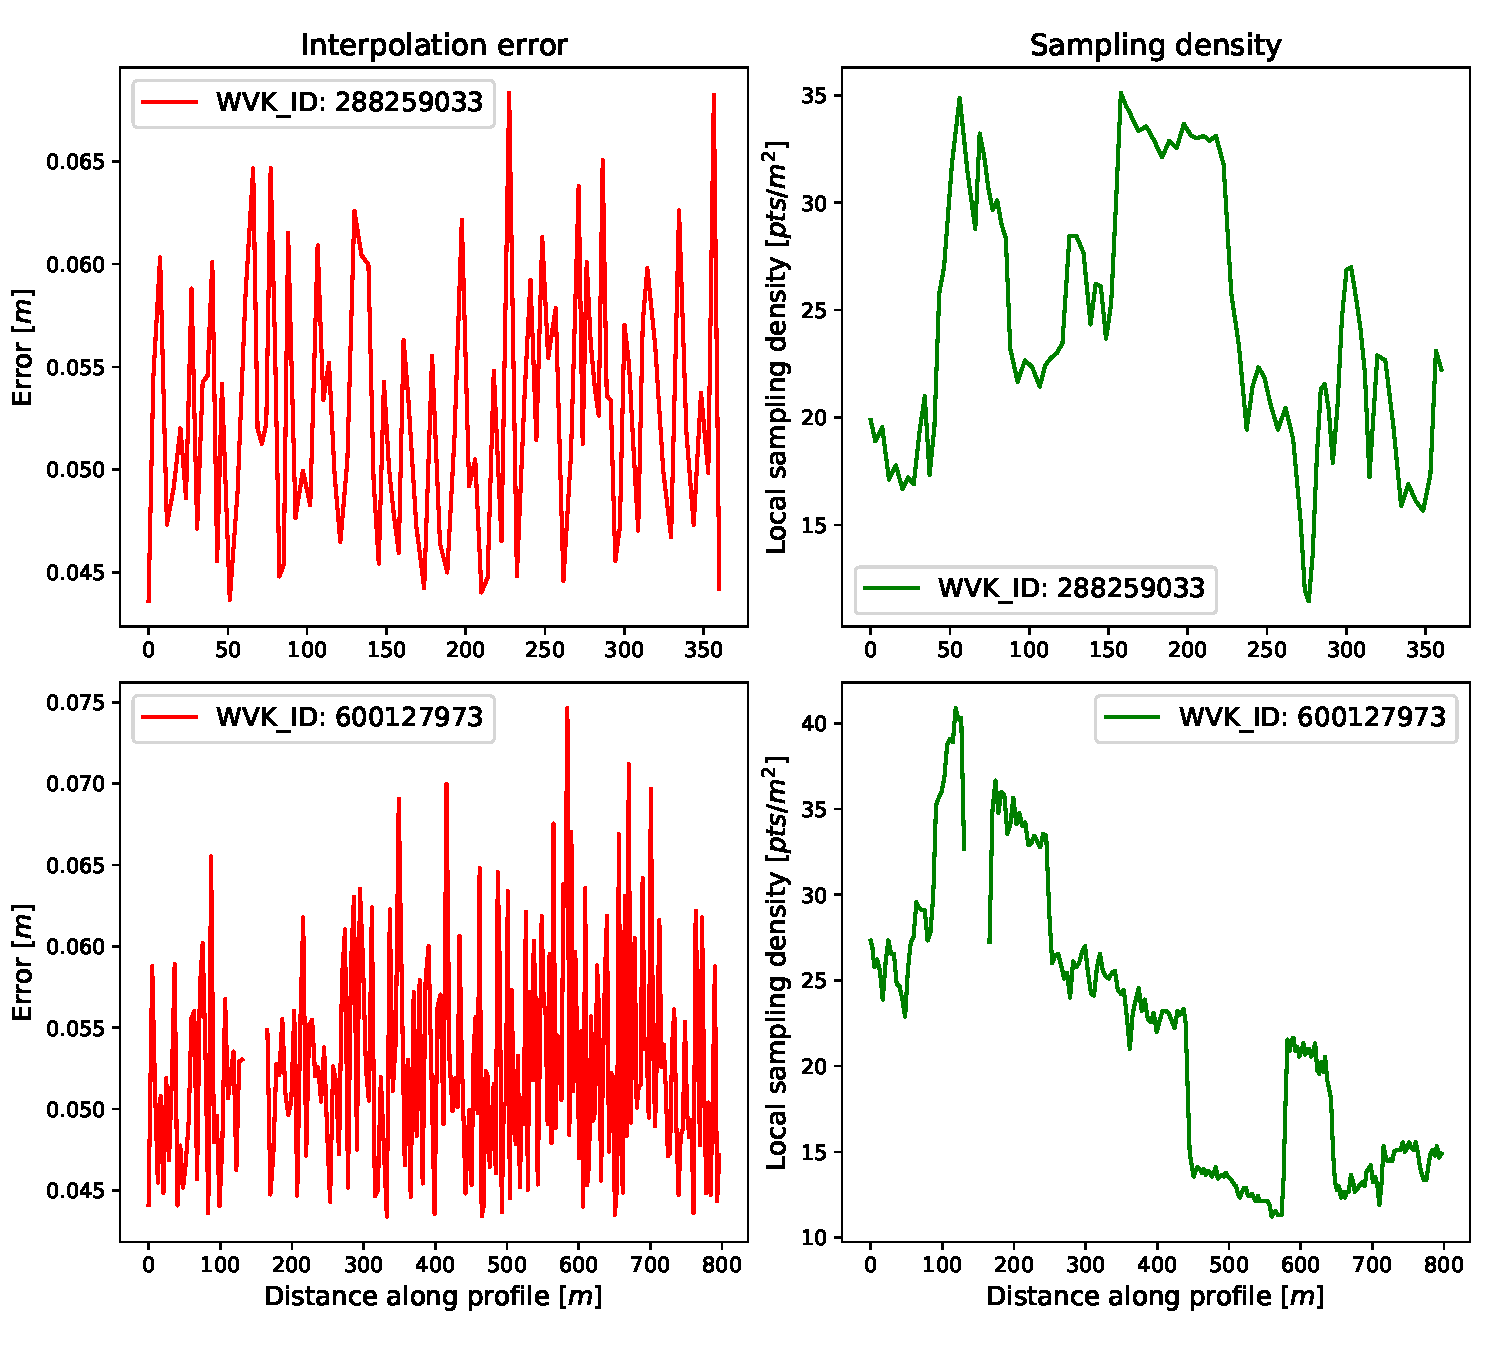
\includegraphics[width=0.9\linewidth]{final_report/figs/formalaccuracy0.pdf}
    \caption{Charts illustrating the formal accuracy assessment results on two \textit{wegvakken}.}
    \label{fig:formalaccuracy0}
\end{figure}

\begin{figure}
    \centering
    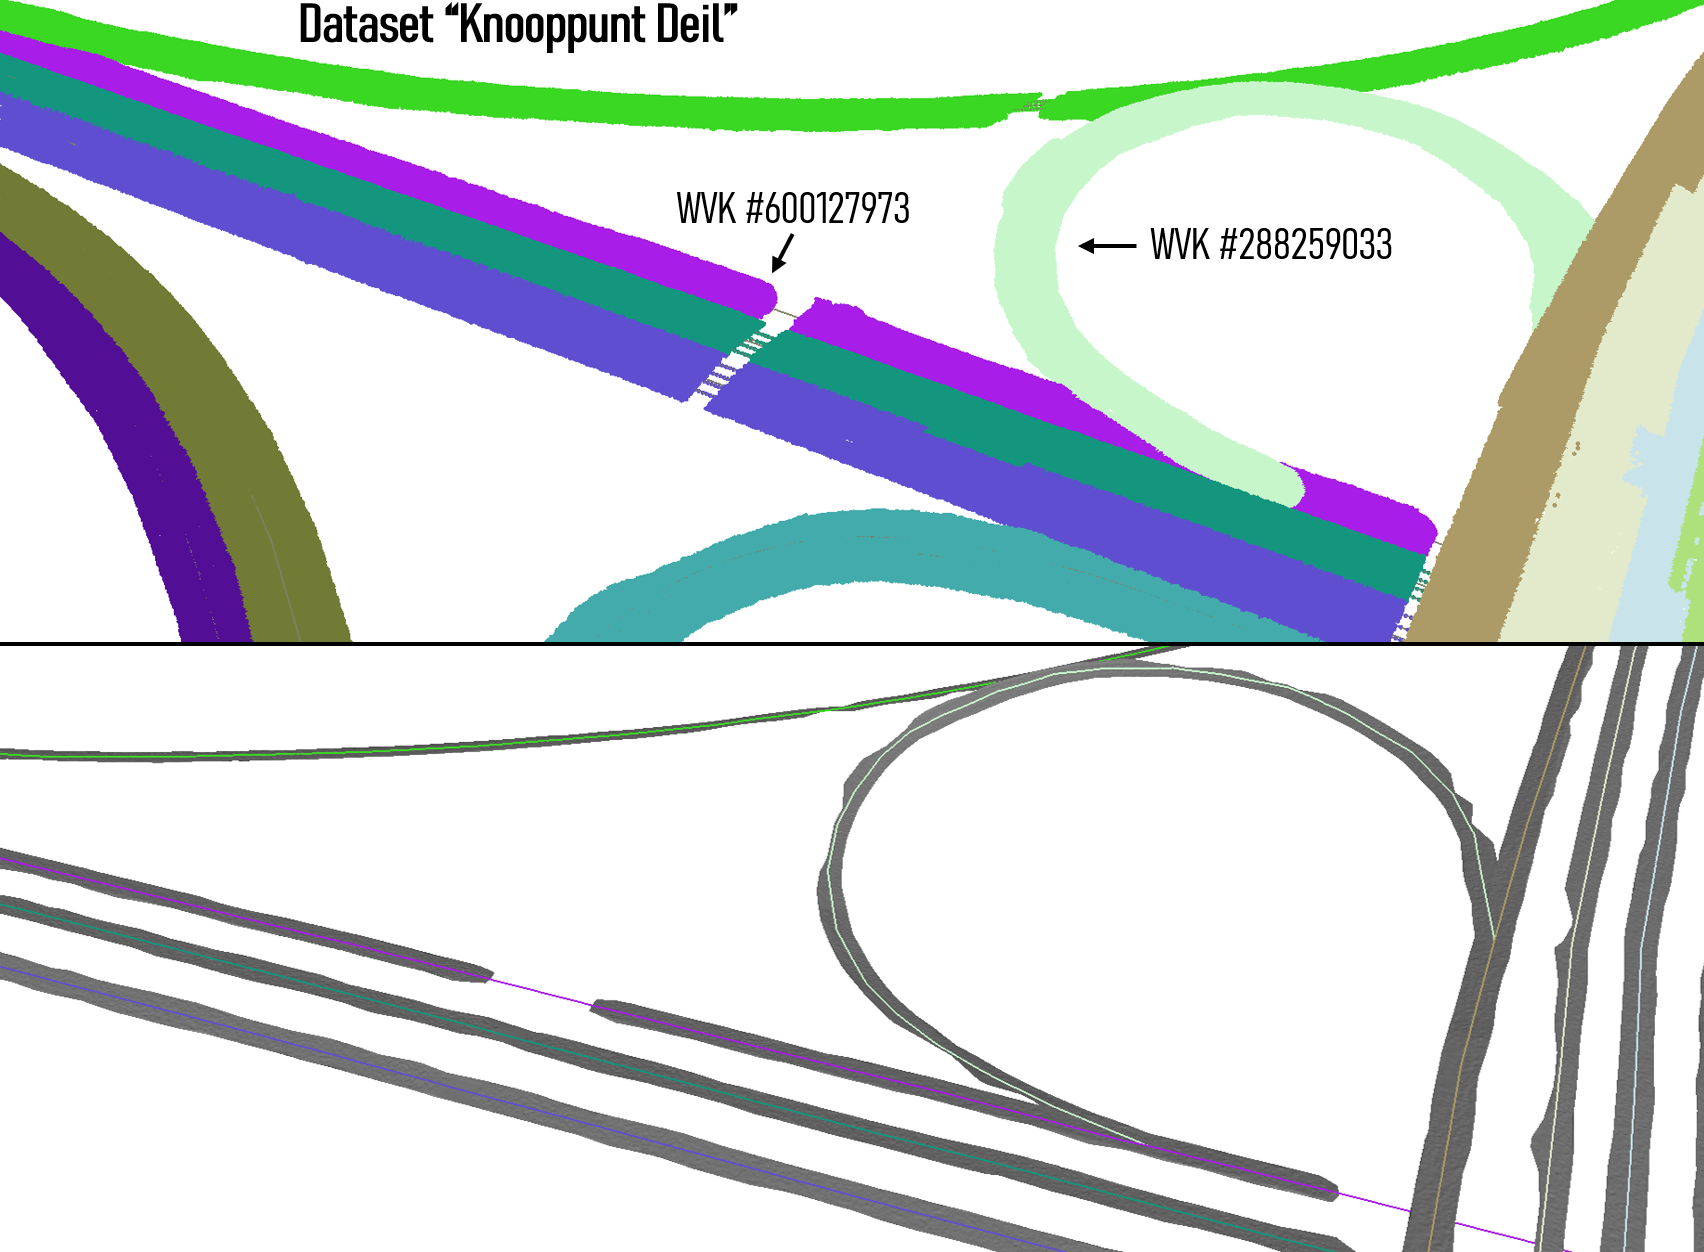
\includegraphics[width=0.9\linewidth]{final_report/figs/formalaccuracy1.png}
    \caption{Visualisations showing the subclouds, \ac{tin}s and 3D-NWB centrelines in the area concerned by Figure \ref{fig:formalaccuracy0}.}
    \label{fig:formalaccuracy1}
\end{figure}

The charts in Figure \ref{fig:formalaccuracy0} show interpolation error profiles from 2 \textit{wegvakken} from our chosen testing dataset. From the lack of a trend in the errors, and their small magnitudes overall, we may deduce that the output accuracy is sufficiently high with respect to the 20-centimetre requirement of \ac{ndw}. Any differences due to the \ac{tin}-linear interpolation represent an \textit{increase} in accuracy relative to the 15 cm elevation accuracy of \ac{ahn3}. The two \textit{wegvakken} shown in the figure exhibit theoretical interpolation elevation errors in a range of about 4 centimetres to 7 centimetres, with mean errors of 5 centimetres for both. The variation is always randomly distributed, because the positions of \ac{nwb} vertices relative to the containing triangles' vertices also lack correlation (which is what controls the value $M$ that determines how much the accuracy is improved). In theory, the only factor that could introduce correlation into these profiles would be roads with very steeply sloping surfaces, but no roads in this dataset (or any of my datasets) reach a slope steep enough to affect the errors significantly, and introduce correlation.

The top part of Figure \ref{fig:formalaccuracy1} shows the 3D geometry of the subclouds and centrelines of the same two \textit{wegvakken}. \textit{Wegvak} \#288259033 has a shape which is representative of the steepest slopes and sharpest bends one can expect from the Dutch road network; it connects a ground-level motorway lane with another one running orthogonal to it directly above, on a bridge. \textit{Wegvak} \#600127973 is the ground-based motorway lane that it connects. It lies entirely flat on the ground, with little to no variation in its elevation. I picked it because its shape is the opposite of that of \#288259033, and because it had been split into two parts due to a 15-20 m long data gap which is visible in the figure. The gap also lacks \ac{dtb} coverage. The bottom image in Figure \ref{fig:formalaccuracy1} shows the corresponding \ac{tin}s, and it is visible in this figure that \ac{nwb} veers to the outer edge of the steep, curved \textit{wegvak}, almost reaching it. The relatively thin width of the \ac{tin} and its rugged outer edge is a result of this; the preliminary edges were constructed partially off-road due to \ac{nwb}'s poor georeferencing.

I added sampling density plots on the right in Figure \ref{fig:formalaccuracy0}. The first important observation to make about these charts is that the data gap in sampling density between 100 and 200 m along the profile in \#600127973 is due to the data gap I mentioned above; here the density is 3 points per m\textsuperscript{2} or less - which is the threshold below which the cut-out happens, i.e. accuracy is not computed - visible in the chart on the left in the same figure. The sharp drops in density around the gap illustrate that the neighbourhood queries already indicate the presence of the gap right before and after reaching the centreline vertices that fall into it. The two \textit{wegvakken} \#288259033 and \#600127973 have mean sampling densities of 24 and 21 points per m\textsuperscript{2} respectively - well above the nominal accuracy of the dataset, primarily owing to the flatness of the road surfaces.

The second important observation is that while local sampling density fluctuates by as much as 80-90\%, it never reaches the minimum threshold in places other than no-data zones and where only \ac{dtb} data is available (the latter is not separately illustrated here). The fluctuation is due to the inhomogeneous sampling rate of \ac{ahn3}. It is already present in the raw point cloud, and is simply a factor of how many times a given area was scanned by the aircraft's laser sensors. The figure was generated from my final results, which all use a thinning factor of 2 - meaning that the values seen in the charts are half of the maximum available. Increasing the thinning factor further may result in the sampling rate dropping below the threshold in certain exposed regions, hence it is not recommended. The results shown in these two charts are representative of all testing tiles; significant deviations from what I described above and what is shown in the figure were not observed elsewhere either.

The third, and last important observation is that neither the recorded sampling rates, nor the theoretical accuracy values are indicative of locations where \ac{nwb}'s 2D georeferencing is poor. While \ac{nwb}'s location is far from the road's real centre in \#288259033, it is not off the road, and as a result the interpolated elevations will still be correct, or at least they will definitely correspond to some part of the road surface. As far as theory is concerned, the elevation is the \textit{correct elevation} at the \textit{incorrect \ac{nwb} location}. This also holds for places where \ac{nwb} is not on the road surface, but in such places both the sampling density and the accuracy may drop, the former because the \ac{tin} construction algorithm is not meant to be used in uneven areas, and the latter because of (and only in the case of) introducing sloping triangles into the \ac{tin}.

The mean error and sampling density of the entire testing dataset are 5 cm and 19 points per m\textsuperscript{2} respectively.

\subsection{Ratio of accurate vertices}
\label{sub:completeness}

The frequency at which the algorithm has to deem output accuracy unknown fluctuates significantly both inside and between testing datasets. How often this happens depends on the number of linearly interpolated values, and how often the sampling density drops below the 3 points per m\textsuperscript{2} threshold. The percentage ratio of accurate vertices varies, under normal circumstances, between 85 and 95\%. Special circumstances (such as tunnels) may further decrease this, which will be discussed in Section \ref{sub:accuracytabulated}.

Where no special circumstances are encountered, variations can be traced back to two main controlling factors: how much of the road network is occluded, how accurate the preliminary elevations are, and how complete \ac{dtb} is in the given testing dataset. The relevance of the amount of occlusion is straightforward to understand: the more the occlusion, the bigger the chances are of encountering an \ac{ahn3} data gap where linear interpolation may need to be used.

The completeness of \ac{dtb} is a factor here because it prevents linear interpolation from being used. However, for the program to consider interpolation accurate locally, \ac{dtb} \textit{also} needs to have good enough coverage. Therefore, only a subset of the \ac{dtb}-covered data gaps will be deemed accurate. \ac{dtb} rarely exists for provincial roads (\ac{p_roads}), hence Lidar data gaps in such roads will \textit{almost always} result in linear interpolation. In turn, this means that data sets comprised primarily of \ac{p_roads} will have lower accurate vertex ratios. Preliminary elevation accuracy is important, because it controls \ac{dtb} coverage. If the preliminary elevations are inaccurate (due to a poor polynomial fit, in most cases), then even if \ac{dtb} exists locally, it may not be found.

As I mentioned in Section \ref{sub:accuracyoverview}, \ac{dtb} is effectively a placeholder for a more accurate dataset in terms of this accuracy assessment workflow. Records of which vertices were affected by \ac{dtb} data are generated by my implementation, and reusers are advised to consider all of these vertices inaccurate due to the temporal issues. For the purposes of this accuracy assessment demonstration, \ac{dtb}-based interpolation with high enough local sampling density was considered accurate and included in the percentage values. However, because \ac{dtb}-based sampling density also reflects the line densification threshold used when converting it to a point cloud (in addition to the number of \ac{dtb} lines available locally), I must emphasise here that \ac{dtb}-based sampling density values are partly artificial.

Linear interpolation is rare outside of \ac{ahn3} data gaps (including those due to occlusion), and especially rare where \ac{nwb}'s georeferencing is correct - in my datasets, 98-100\% of non-occluded vertices are interpolated in the underlying \ac{tin}s. The majority of these are due to the rare cases where too many cross-sections are skipped during preliminary edge estimation, preventing proper \ac{tin}s from being constructed locally.

\subsection{TIN completeness}
\label{sub:tincompleteness}

\begin{figure}[h]
    \centering
    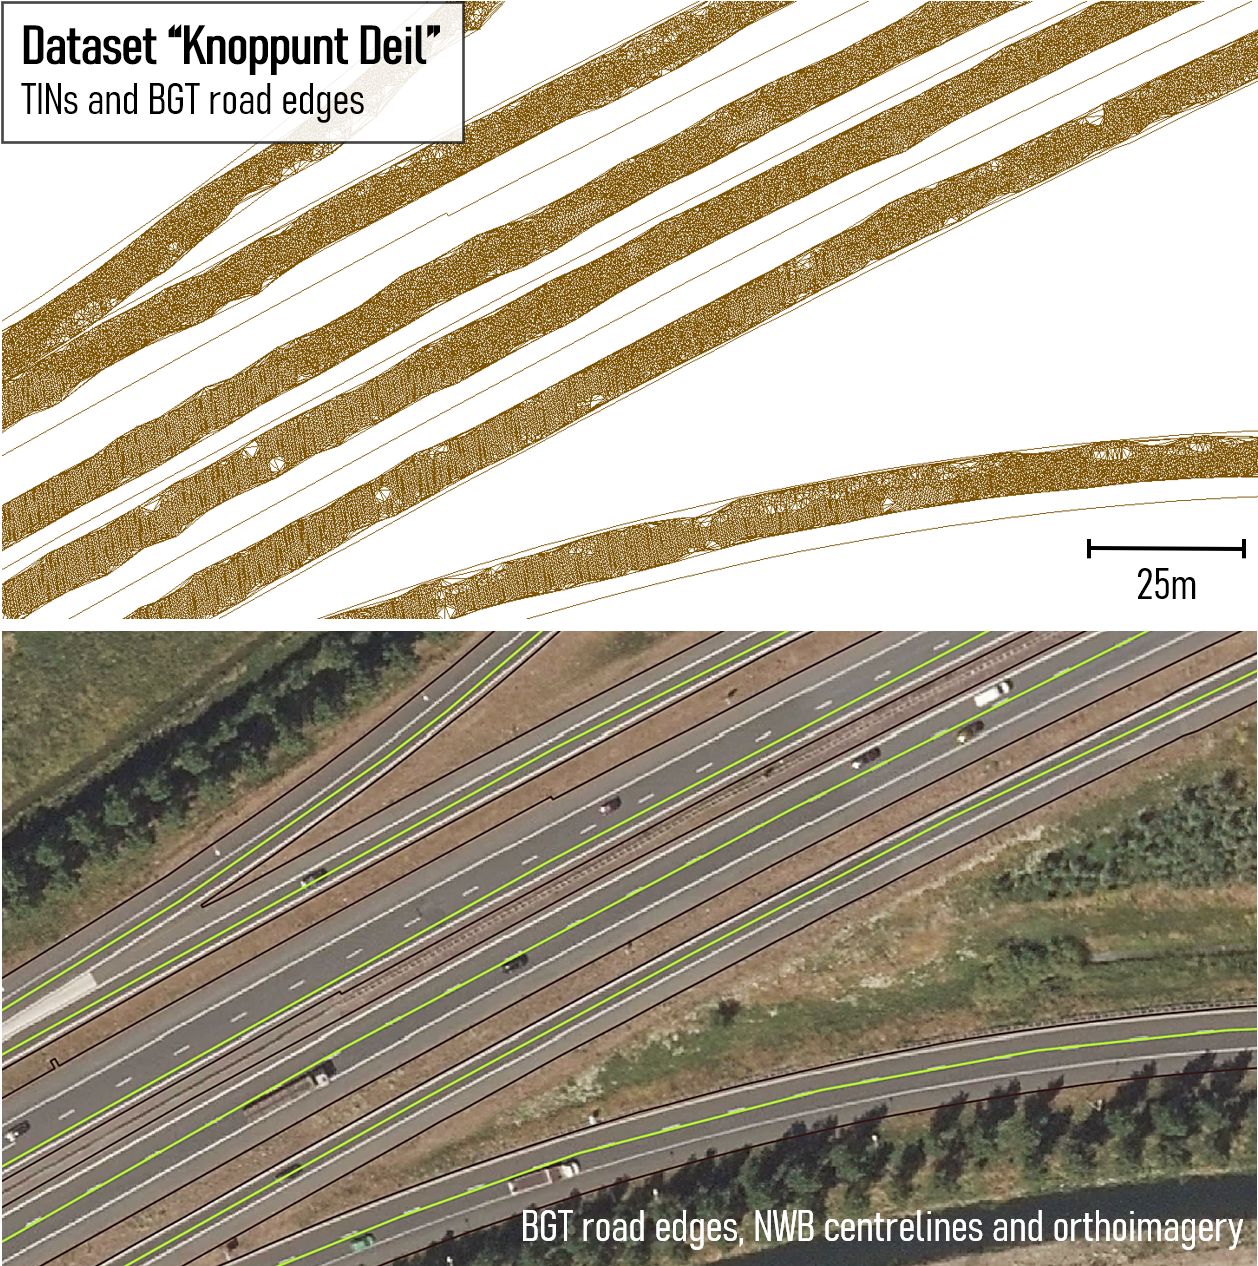
\includegraphics[width=0.8\linewidth]{final_report/figs/bgtcomparison.png}
    \caption{2D Visualisations comparing \ac{bgt} road edges with the \ac{tin}s, with \ac{nwb} centrelines and with Luchtfoto 2020 satellite imagery.}
    \label{fig:bgtcomparison}
\end{figure}

As I mentioned in the methods section, I evaluated the completeness of the \ac{tin} road surface models via a comparison with \ac{bgt} polygons. Figure \ref{fig:bgtcomparison} below shows the results of one such comparison, which I deemed representative of the relationship overall. The top part of the figure shows some of the \ac{tin}s overlain on the outlines of \ac{bgt} geometries, which allows one to see how well the \ac{tin}s agree with these reference geometries. The bottom half of the figure, in turn, compares the \ac{bgt} geometries to satellite imagery - to verify how well \ac{bgt} itself agrees with what we can consider an accurate representation of the visual appearance of these roads. The orthoimagery is from the 2020 edition of Kadaster's Luchtfoto dataset, available as open data like all other datasets used in this research.

The \ac{nwb} centrelines are also shown here to demonstrate the extent of the georeferencing issues relative to \ac{bgt} and to the orthoimagery. The poor agreement is the result of two factors combined: \ac{nwb} approximates the centre of the traffic-occupied road surfaces rather than the paved surfaces, and its georeferencing is inaccurate in general. The definition of traffic-occupied road surfaces excludes hard shoulders. If the traffic-occupied surface is on one edge of the full paved surface, \ac{nwb}'s poor georeferencing is more likely to cause it to be close to, or beyond the real edge of the paved surface.

\ac{bgt}, on the other hand, appears to be an accurate 2D representation of the paved road surfaces. Its extents do not, however, correspond to that which I can \textit{typically} model reliably using the pipeline I developed. Ideally, the surface model should cover the entire paved area, but as I described in Section \ref{sub:m_edgeapproximation}, I found using a maximum road width to be the only viable means to ensure that my approach works in most cases. The \ac{tin} extensions that are part of the \ac{tin} construction step (Section \ref{sub:m_tinconstruction}) mitigate this issue to a certain extent, but they do not eliminate it entirely. Allowing the \ac{tin} extension to go too far beyond the preliminary/optimised edges increases the chances of extending the roads into unwanted areas, and increases runtimes significantly.

Motorways with hard shoulders, which are shown in the centre of Figure \ref{fig:bgtcomparison}, are particularly difficult to handle because the hard shoulders and potential extra lanes extend their width far beyond that, which could be reasonably expected from municipal roads and dual carriageways - which is what my parametrisation prioritises. A solution to this issue could be to automatically select pre-set configurations of the parametrisation appropriate to each road type, but this is not an area that my research explored.

The \ac{tin} models in the top part of the figure show that the \ac{tin}s are in good agreement with the \ac{bgt} geometries. The same issues which I described in Section \ref{sub:r_tinconstruction} are also manifested here, for instance the on-ramp model in the top of the image contains some off-road points where both \ac{nwb} and \ac{bgt} appear to veer too far from their ideal positions. In general, based on examining all my results, I estimated that the \ac{tin} surfaces cover approximately 95\% of the traffic-occupied surfaces found in my testing datasets, and about 75\% of the total paved surfaces as shown by \ac{bgt}. The only major issue appears to be the one I mentioned above, that the full extent of the paved surfaces cannot be modelled without dynamically adjusting the parametrisation of the pipeline's algorithms.

Figure \ref{fig:bgtcomparison} is also illustrative in terms of showing just how detailed these \ac{tin} models are, even with an input thinning factor of 2 for \ac{ahn3}. On the scale shown in this image, and in comparison with the orthoimagery, it becomes visually perceptible that the road surfaces are being oversampled by inserting so many points into the \ac{tin}s.

\subsection{Tabulated values}
\label{sub:accuracytabulated}

In the sections above, I focused on assessing the accuracy and completeness of specific LineStrings (\textit{wegvakken}) in one testing dataset. In Table \ref{tab:accuracytabulated}, I present mean error, sampling density and accurate output vertex ratio values for \textit{all} my testing datasets.

Almost no variation is observed in the mean \textbf{formal output vertical error} across the datasets. As explained in the sections above, this is due to the fact that propagating errors through the interpolation technique only exhibits large (positive) fluctuations in the output error when steep triangles are encountered. The first row of tabulated values thereby represent evidence that triangles steep enough to affect accuracy are decidedly rare in our \ac{tin}s, and the output accuracy is, in effect, roughly constant and almost entirely determined by the input accuracy.

The \textbf{sampling density} values show that the density of points is reliably high, consistently staying well above the threshold, below which accuracy is deemed undetermined. However, large variations are still observable between the testing datasets, with values ranging from about 14 to 27 points per m\textsuperscript{2}. The variation has several reasons based on my analysis, each with non-negligible influence. The first reason is that the stock sampling density of \ac{ahn3} appears to vary on a large scale, in various parts of the country, and also locally, which I have already shown in Figure \ref{fig:formalaccuracy0}. The second reason is that accuracy is computed based on radial queries around \ac{nwb} vertices, and will therefore show lower values for very thin roads where \ac{nwb} is close to the edge of the road.

Lastly - but most importantly for us - it gives an indication of the pervasiveness of occlusion. Partial occlusion (due to vegetation) and complete occlusion (due to bridges and other opaque structures) decrease the \ac{tin} vertex density significantly. For instance, the low value seen in 33CN2 (\textit{Hoenderloo}) is primarly due to the road being situated in a dense, old-growth forest, and the one in 37HN2 (\textit{Knooppunt Ridderkerk}) is mainly due to occlusion resulting from the roads passing above and below one another in the motorway junction.

However, the medium value seen in 25BZ2 (Amsterdam Hemhavens) does \textit{not} reflect the fact that there is a sizeable tunnel in the dataset. Since the tunnel has no \ac{dtb} line coverage, the relevant \ac{nbrs} part's \ac{tin}s do not extend into the tunnel. As I explained in the sections above, these densities are computed from the \ac{tin}s, and therefore road sections without \ac{ahn3} and \ac{dtb} coverage are not allowed to affect these sampling density measurements. I made this design choice because in these areas, my implementation simply interpolates output elevations via linear interpolation. Therefore, these areas do not, strictly speaking, constitute areas in which we can predict elevation with any certainty, especially not where they are long, such as the tunnel in this particular testing tile. Although I am providing linearly interpolated output values in these regions, I essentially consider them to be excluded from my analysis, and thus I also exclude them from the density computations.

The presence of the tunnel can still be recognised in the \textbf{accurate vertex ratio} row in Table \ref{sub:accuracytabulated}. The lower value seen for 25BZ2 is simply due to the tunnel - almost all other parts of the roads in this dataset have detailed \ac{tin}s associated with them. In this row, there is another value that stands out. The rest of the ratios show that between about 85\% and 95\% of the output vertices have reliable, estimated accuracy, whereas this ratio is only 56\% in the case of dataset 37EZ1 (\textit{Rotterdam Ketheltunnel}). This is the combined result of two factors: as the name implies, this dataset also contains a tunnel. But, as Table \ref{tab:inventory} mentions, the \ac{ahn3} data pre-dates the completion of the tunnel and the surrounding parts of the motorway, and as a result, part of the output is corrupted. Already during preliminary elevation estimation, the standard deviations are a magnitude larger than those encountered in other locations, because the construction works do not represent a smooth surface. In the Lidar segmentation step, the roads are split into many small \ac{nbrs} parts, with much of the road thereby becoming flagged for linear interpolation. As a result, many of the \ac{nwb} vertices' accuracy will be deemed unknown. This issue could be resolved in this case, if the large standard deviation in the preliminary elevation estimation triggered an alternative workflow in which only the support dataset is used in the region in which the primary data is unreliable. Developing and implementing such a workflow was not part of this research, hence it is further discussed in Section \ref{sec:futurework} in the context of recommended future work.

\begin{table}
    \resizebox{\linewidth}{!}{\begin{tabular}{@{}p{1cm}lllllllllll@{}}
        \toprule
        \multicolumn{1}{c}{}    & 20BN1 & 25BZ2 & 25DN2 & 32BN1 & 32FZ2 & 32HZ2 & 33CN2 & 37EZ1 & 37HN2 & 38GZ1 & 39CZ1 \\ \midrule
        A                       & 5.26  & 5.26  & 5.30  & 5.27  & 5.28  & 5.30  & 5.28  & 5.36  & 5.30  & 5.30  & 5.30  \\
        B                       & 26.82 & 19.81 & 20.05 & 14.89 & 16.58 & 14.96 & 16.20 & 13.54 & 13.78 & 15.49 & 19.29 \\
        C                       & 93.03 & 76.15 & 95.09 & 91.74 & 95.51 & 94.21 & 90.52 & 56.26 & 85.25 & 89.09 & 91.73 \\ \bottomrule
        \multicolumn{12}{c}{A = Mean error [$cm$], B = Mean sampling density [$pts/m^2$], C = Accurate ratio as \% of all vertices}
    \end{tabular}}
    \caption{Tabulated 3D-NWB accuracy and completeness results per testing dataset.
    \label{tab:accuracytabulated}}
\end{table}

The values in the bottom row of the table are sometimes slightly lower than I would have expected. For instance 85\% for the 37HN2 (\textit{Knooppunt Ridderkerk}) dataset seemed to me to be too low, because almost all gaps have good \ac{dtb} coverage, and \ac{nwb} almost never misses the \ac{tin}s. The reason why this value is lower than expected is because there are many \ac{ahn3} data gaps, and the point density in the \ac{dtb}-defined parts of the \ac{tin}s appears to consistently miss the minimum above which the vertices would be deemed accurate. The process also appears to sometimes filter out vertices that were interpolated in locations where although \ac{dtb} was "sparse", it still managed to characterise the road surface quite well. This further suggests that it would be better if the decisions regarding where to trust \ac{dtb} were not based on the same type of evaluation as \ac{ahn3}, and were instead based on the geometric layout of the \ac{dtb} lines. While this would indeed improve the accuracy assessment results, it would also mean that the procedure would become specialised to \ac{dtb}, and would not work with other types of support datasets. This is elaborated in more detail in Section \ref{sec:futurework}.

Some of the \ac{nwb} centrelines overshoot the Lidar testing tile extents by up to 20-50 metres. These were left in some of the testing tiles deliberately, to test certain aspects of the the behaviour of the algorithms (as also mentioned in Section \ref{sec:manualpreprocessing}). These can further decrease the accurate vertex ratios by about 2-4\% artificially. The overshoots are visible in Figure \ref{fig:manualpreprocessing}.

\begin{figure}[h]
    \centering
    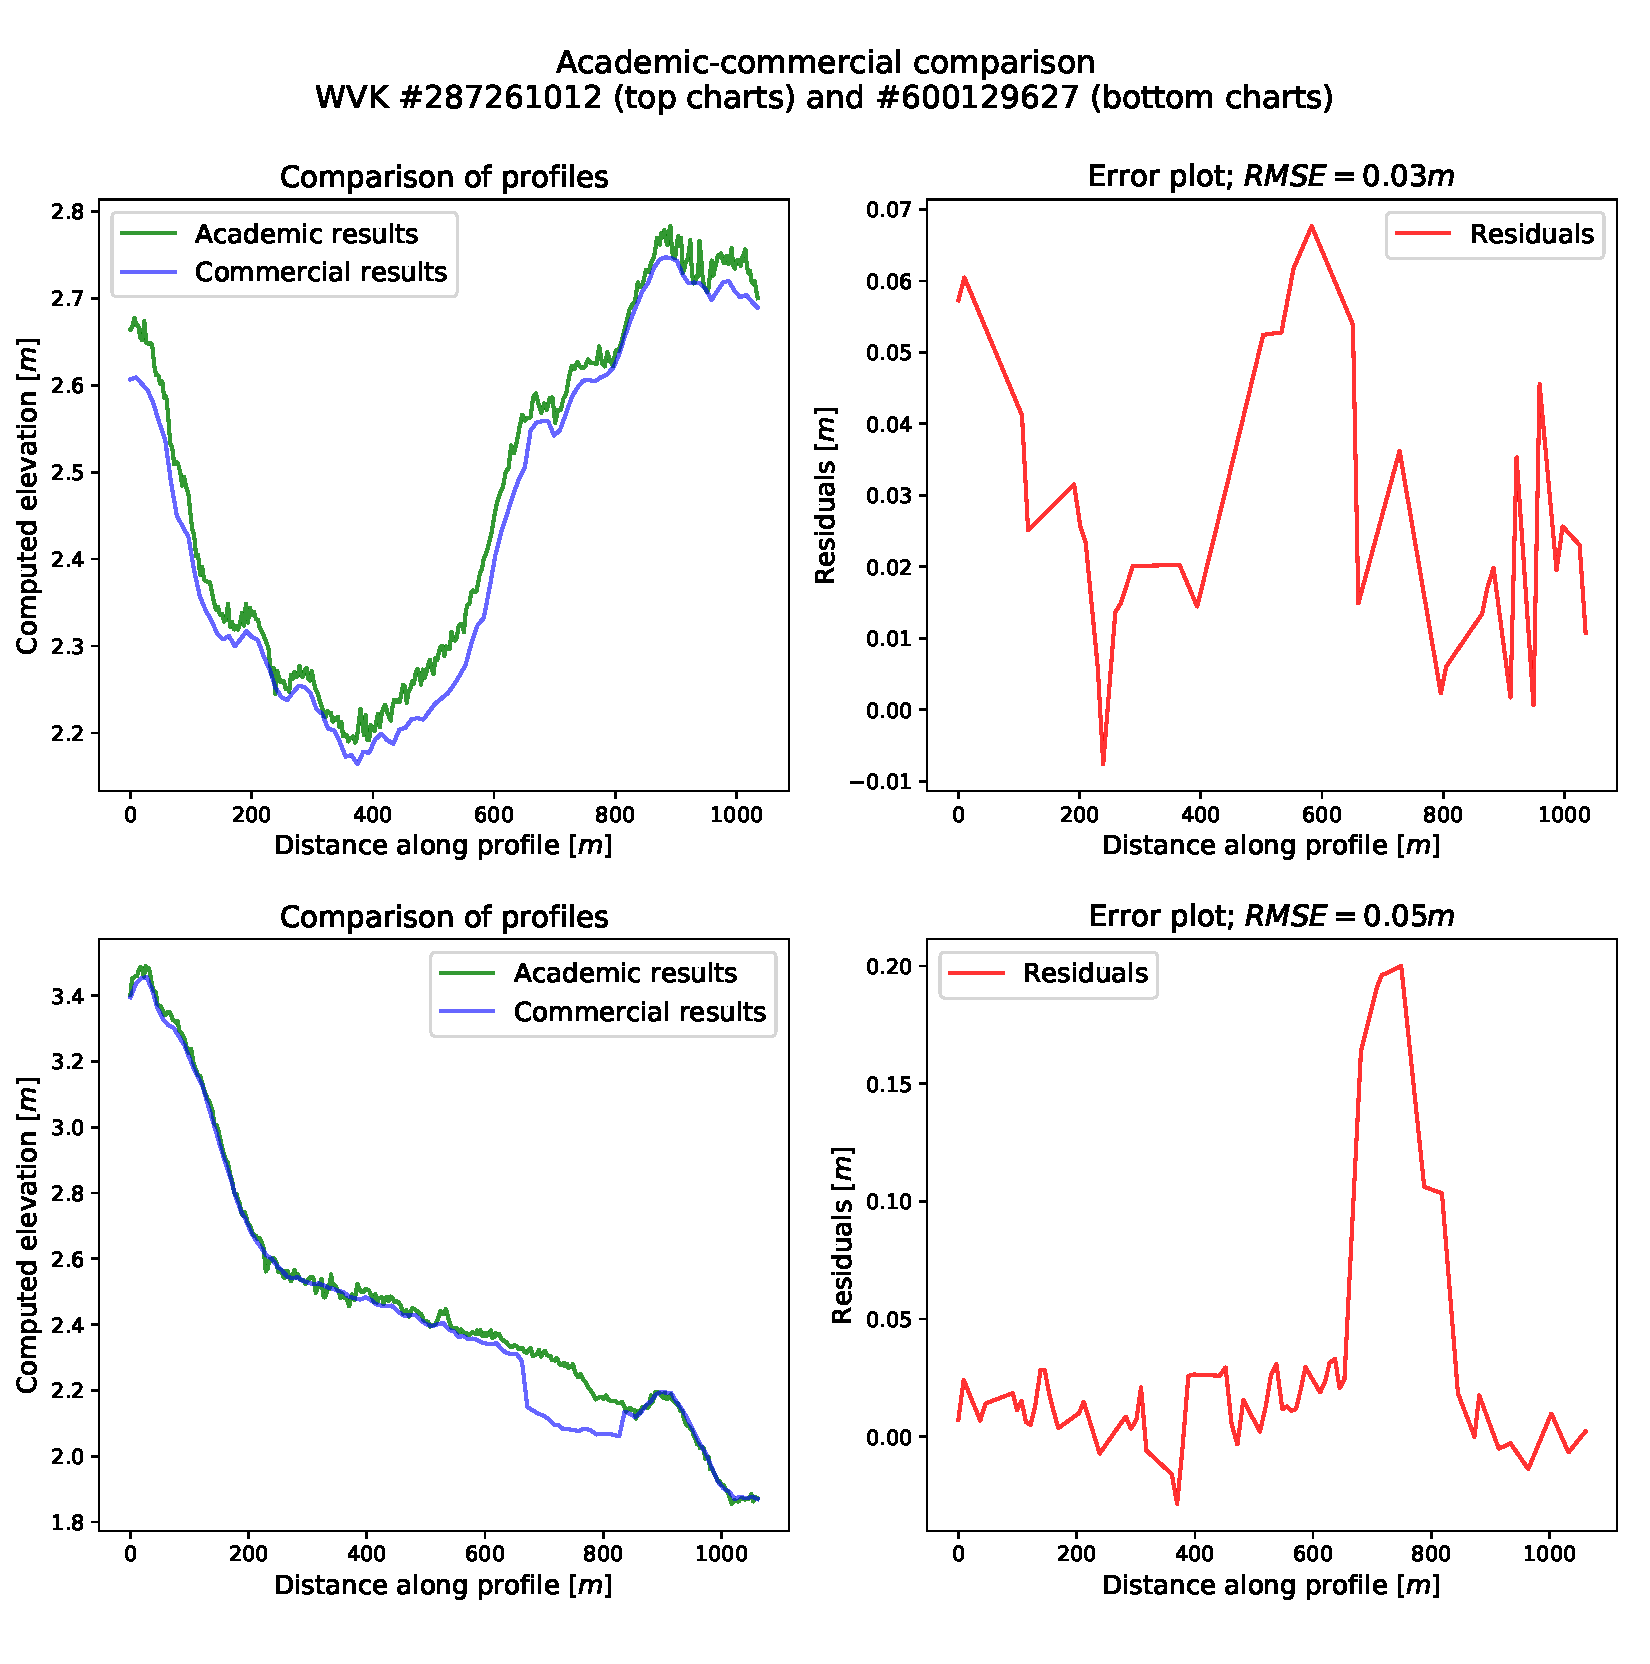
\includegraphics[width=0.87\linewidth]{final_report/figs/commercialcomparison0.pdf}
    \caption{Charts comparing the academic and commercial results using two \textit{wegvakken} from \textit{Knooppunt Deil}.}
    \label{fig:commercialcomparison0}
\end{figure}

\section{Comparison with commercial implementation}
\label{sec:r_comparison}

Like in the accuracy assessment above, I picked some specific \textit{wegvakken} that are particularly representative of the overall results of this comparison. However, here I did not restrict the selection to be from the \textit{Knooppunt Deil} dataset, because the results are very different across my set of testing datasets. Where the agreement is good, the two sets of results can be similar to a degree where it is difficult to tell them apart in a 3D visualisation, unless the Z axis is grossly exaggerated. Examining the correspondence on 2D charts (see Figures \ref{fig:commercialcomparison0}, \ref{fig:commercialcomparison1} and \ref{fig:commercialcomparison2}) works far better in terms of characterising the nature of both the small-scale and large-scale differences that are typically observed when comparing the two datasets. For this reason, I opted to show only 2D visualisations in this section. I also present tabulated mean \ac{rmse} values for all testing datasets in Section \ref{sub:comparisontabulated}.

\subsection{Representative example comparisons}
\label{sub:comparisonexamples}

\subsubsection{Knooppunt Deil}

The top chart in Figure \ref{fig:commercialcomparison0} shows a LineString (\textit{wegvak}) in which the \ac{rmse} between the two datasets is only 3 cm. The \textit{Knooppunt Deil} dataset, from where these LineStrings in this figure were taken, shows exceptionally good agreement between the results and a 3 to 5 cm \ac{rmse} can be regarded as typical everywhere in it. Such a small disagreement could be deemed unimportant, unless systematic - however, in this case there appears to be a small systematic component to it. Notably my results seem to consistently estimate higher elevations for the roads than the commercial ones here. The reason for the systematic nature of these differences is that this LineString represents a motorway, and the commercial implementation always takes motorway elevations from \ac{dtb} where it has coverage. My implementation does the opposite; it prioritises \ac{ahn3}. As a result, the systematic differences between \ac{dtb} and \ac{ahn3} are manifested in these 2D profiles. This is further illustrated by the residuals dropping to almost zero in one place at around 220 metres along the profile, and then for about 50 metres starting at 800 metres along the profile. Here, the chosen \textit{wegvak} passes underneath bridges, hence my implementation also used \ac{dtb} here - thereby triggering near-perfect agreement with the commercial results. Since the absolute value of these systematic differences is minuscule in this location, it can be regarded as unimportant.

In this particular dataset, the agreement between the two datasets is almost always this good - the one exception I found is shown in the bottom charts in Figure \ref{fig:commercialcomparison0}. The difference represents a roughly 20-centimetre erratic drop in elevation in the commercial results. I could not explain this blunder by looking at the input data, hence it must have been introduced by the commercial processing pipeline. The error is large enough to break compliance with the 20-centimetre accuracy requirement of \ac{ndw}, but it is an isolated issue - I have not found other examples of it.

\subsubsection{Gorinchem}

Both \textit{wegvakken} in Figure \ref{fig:commercialcomparison1} were taken from \textit{provincial} roads in the \textit{Gorinchem} dataset. The top two charts were generated from a LineString that is situated in a well-exposed area, free of occlusions. While the \ac{rmse} is extremely low - as in the previous figure - we may notice that here a systematic deviation can also \textit{not} be observed at all. This is because the commercial implementation uses \ac{ahn3} \textit{rasters} to interpolate elevations. Although this does not affect the \ac{rmse}, it is evident from this chart that the commercial results are less detailed than the academic ones. This is simply the result of the academic results using 10-metre vertex densification, whereas my final results were generated using 5-metre vertex densification. Both result in much denser elevation profiles than the original \ac{nwb} vertices would allow, which is the sampling density that the residual plots reflect.

While it might first appear to the reader that the agreement for provincial roads is even better than that for motorways, this is in fact not the case. The commercial solution has no feature implemented to intelligently switch between \ac{ahn3} and \ac{dtb}, and also lacks a set of features that could enable it to handle occlusion correctly in the absence of \ac{dtb}. I illustrate both of these limitations in the bottom two charts in Figure \ref{fig:commercialcomparison1}. Between about 330 and 420 metres along the profile, the commercial results show a sudden elevation increase, while the academic ones show a (much smaller) abrupt change in the opposite direction. Everywhere else in the \textit{wegvak}, the agreement is at least as good as in the top chart.

This artefact is created by the combination of the above missing features in the commercial software. At this location, the provincial road from which the \textit{wegvak} is taken, passes underneath a series of bridges. At this location, the \ac{ahn3} rasters simply record the elevation of the surfaces \textit{on} these bridges, hence this is what appears in the commercial outputs. This represents an approximately 5 m systematic overestimation of elevations over just under a 100 metres of distance along this road. My results, on the other hand, underestimate the elevations in this zone by about 30 to 40 centimetres. This is not an issue with the academic methods or implementation, it is due to \ac{dtb} being outdated locally. For this particular set of provincial roads, \ac{dtb} exists because of their proximity to motorways - in general, provincial roads do not have \ac{dtb} coverage. My implementation recognised the presence of \ac{dtb} lines, and made use of them.

The \ac{dtb} data was close enough to the predicted elevation of the road for my implementation to deem it reliable. However, inspecting them on this 2D elevation profile reveals that \ac{dtb} is, locally, itself underestimating the elevation of the road. This can be explained by the temporal difference between \ac{ahn3} and \ac{dtb} locally. Had there been accurate support data available, my implementation would have produced correct results - and even in the absence of support data, it would have interpolated linearly across the region, which still represents a better solution than including the outliers the way the commercial results do.

\begin{figure}
    \centering
    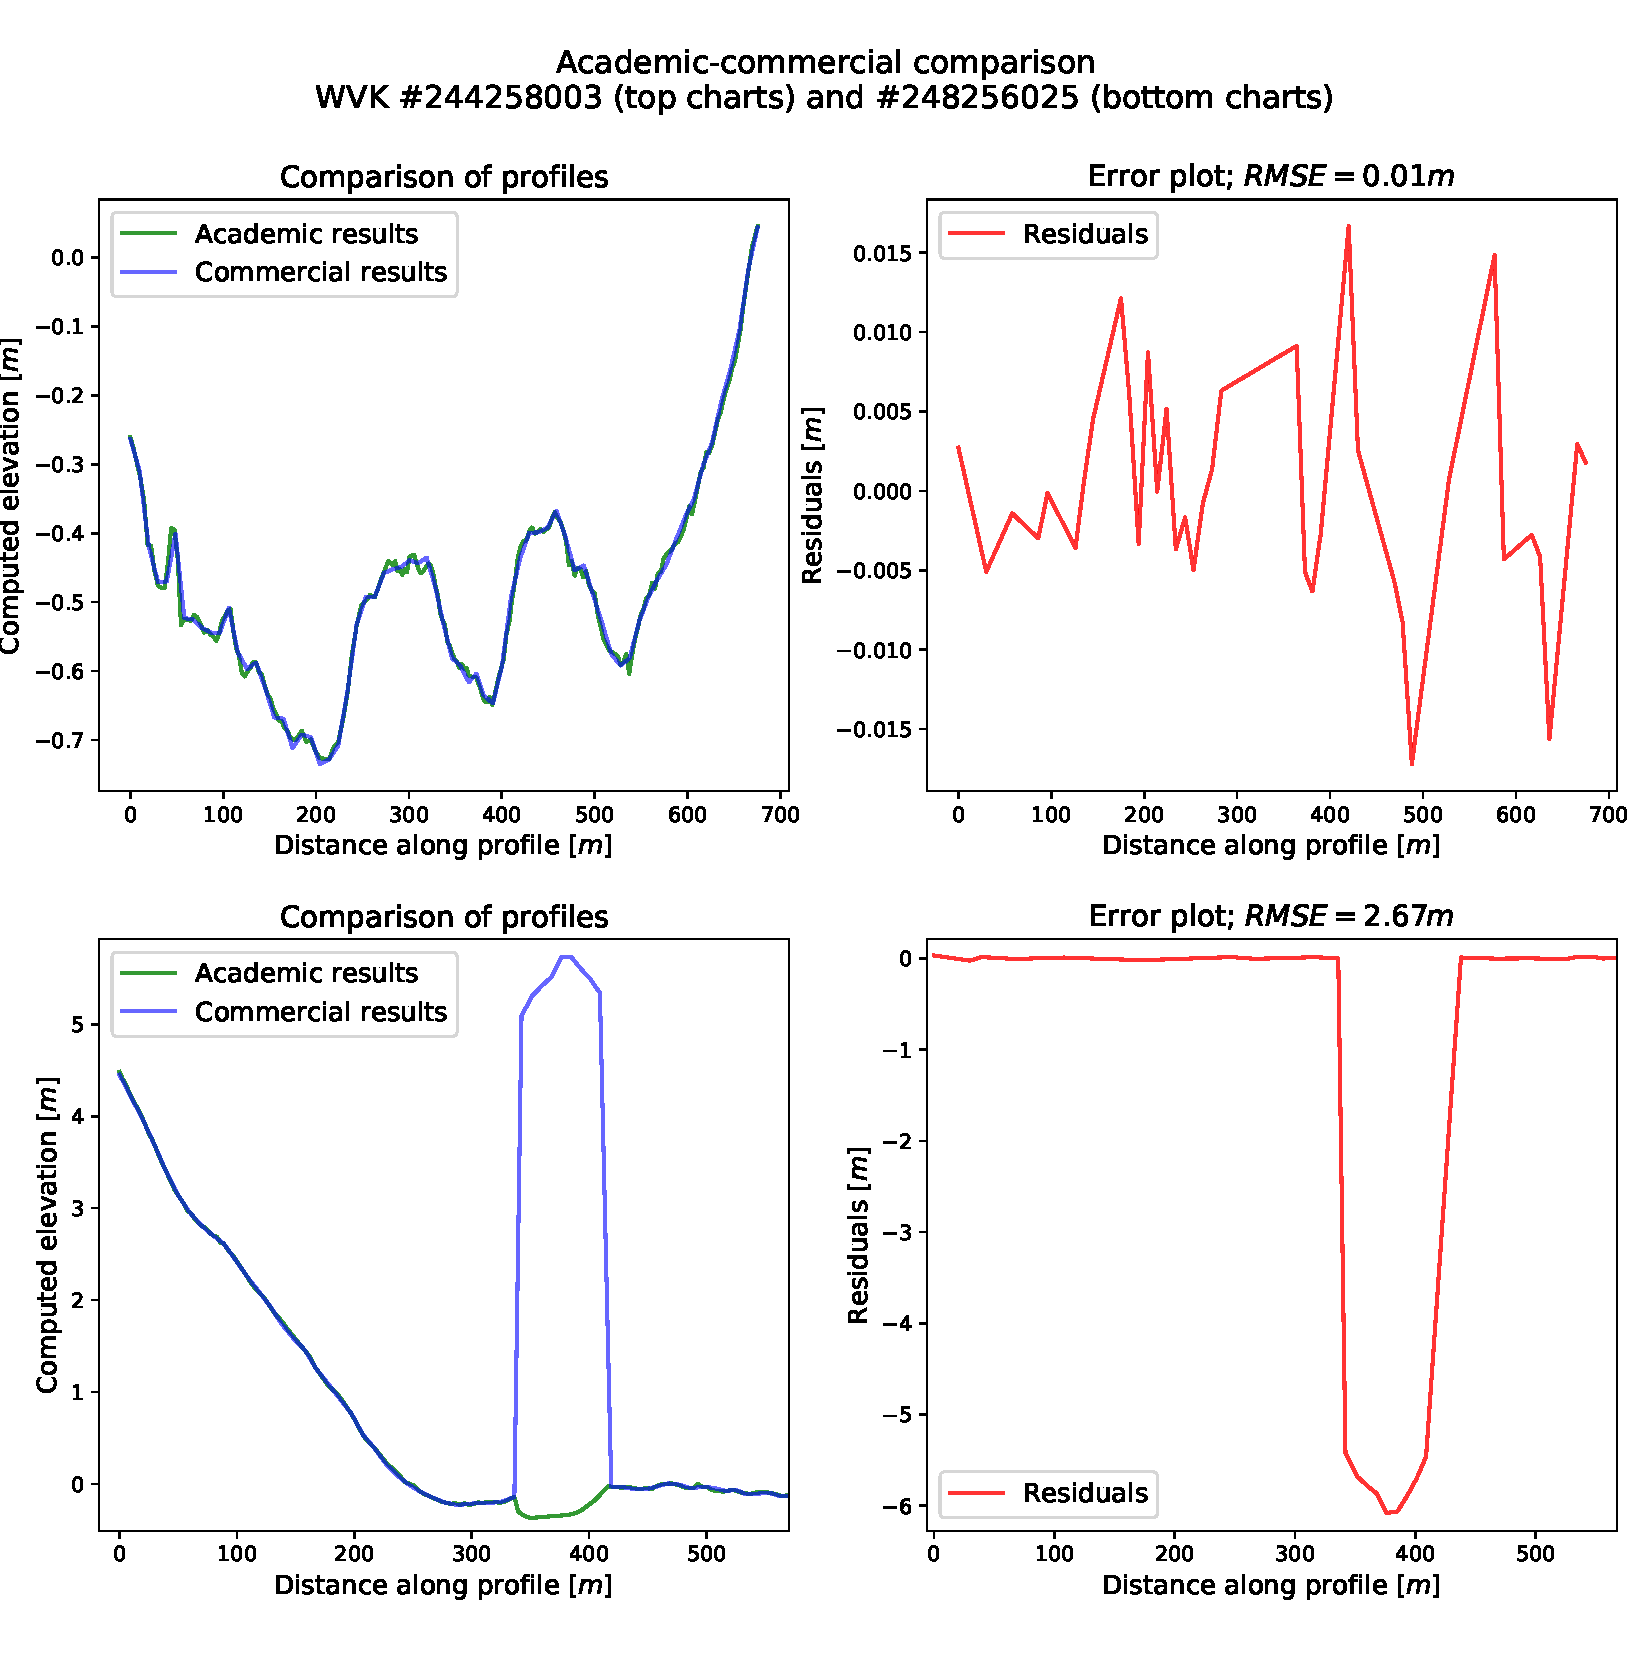
\includegraphics[width=0.87\linewidth]{final_report/figs/commercialcomparison1.pdf}
    \caption{Charts comparing the academic and commercial results using two \textit{wegvakken} from dataset \textit{Gorinchem}.}
    \label{fig:commercialcomparison1}
\end{figure}

\subsubsection{Knooppunt Ridderkerk}

Figure \ref{fig:commercialcomparison2} shows motorway \textit{wegvakken} taken from the \textit{Knooppunt Ridderkerk} dataset. The reader might recall that I used this dataset as an example of where the temporal differences between \ac{dtb} and \ac{ahn3} give rise to significant disagreements between the road elevations they contain. This last comparison figure serves to illustrate that this gives rise to significant differences between the commercial and academic results.

The outdated elevations in \ac{dtb} are the only ones considered by the commercial implementation, which results in elevations being consistently overestimated by up to half a metre relative to \ac{ahn3}, and therefore also my results. Good agreement between the two sets of results only emerges where my implementation also resorted to using \ac{dtb}, because \ac{ahn3} was missing locally. This is the same phenomenon that caused the small, systematic deviations in Figure \ref{fig:commercialcomparison0}, the only difference is that \ac{dtb} is more affected by the temporal issues here, than there.

This demonstrates the flaws in \ac{ndw}'s unconditional assumption that \ac{dtb} is more accurate spatially and temporally than \ac{ahn3}, especially from a temporal updates perspective. They specifically opted to prioritise its use as it is updated far more frequently than \ac{ahn3}. However, this assumption likely did not consider the fact that the updates only concern roads that underwent refurbishment, upgrades or other modifications, and roads that were newly built. Otherwise, the position of \ac{dtb}'s line features is \textit{not} re-measured regularly, as I also mentioned in Section \ref{sub:dtb}. These outdated elevations represent a further disparity between the noise regulations' requirements and the commercial implementation, and they affect the results in the \textit{Knooppunt Ridderkerk} area significantly.

\begin{figure}
    \centering
    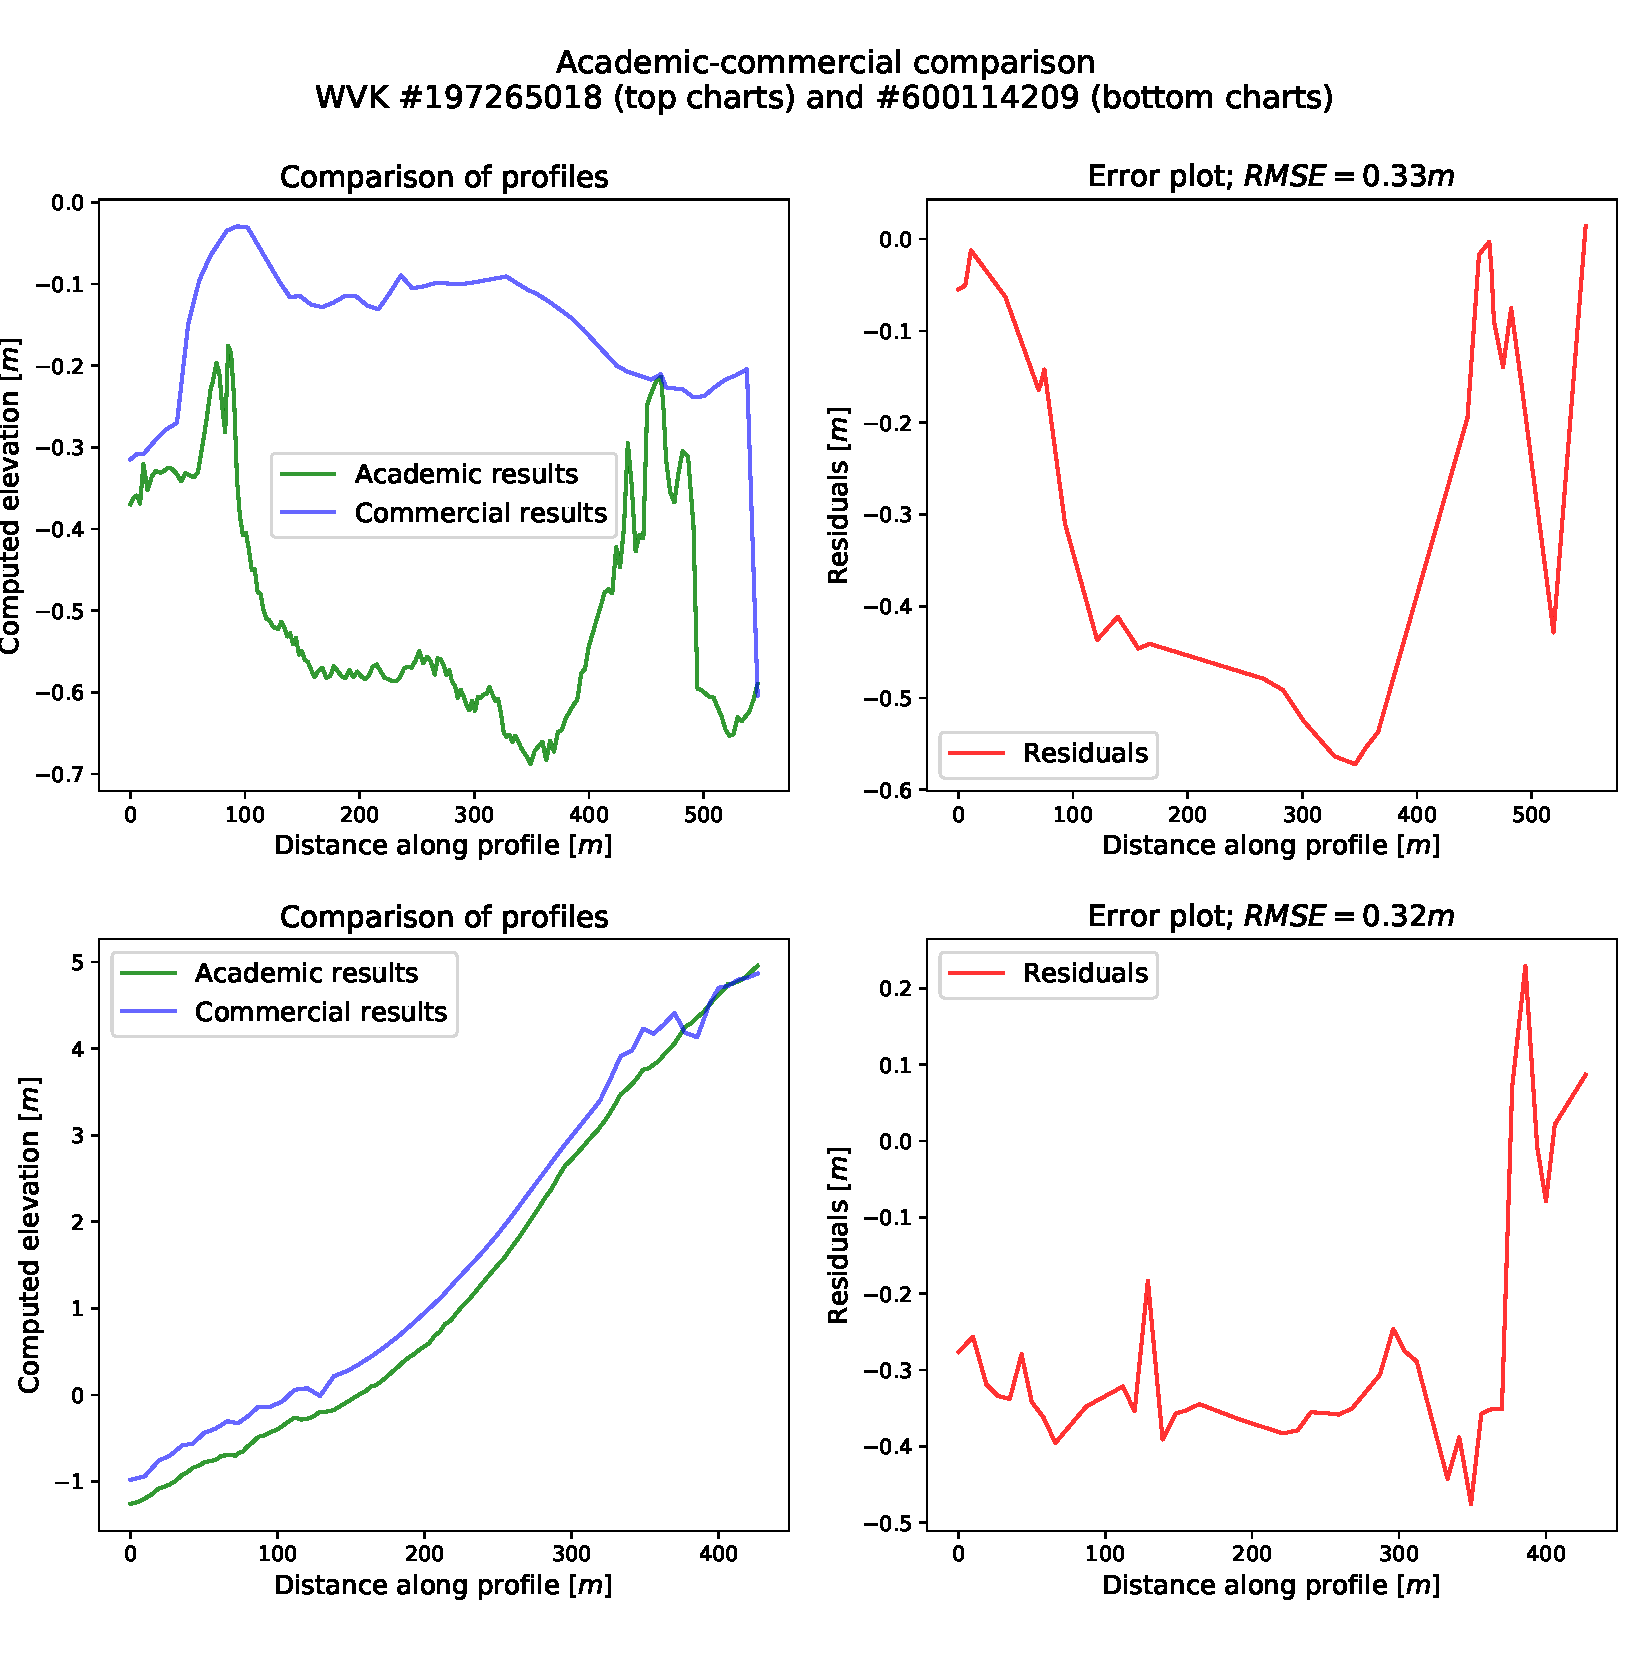
\includegraphics[width=0.87\linewidth]{final_report/figs/commercialcomparison2.pdf}
    \caption{Charts comparing the academic and commercial results using two \textit{wegvakken} from dataset \textit{Knooppunt Ridderkerk}.}
    \label{fig:commercialcomparison2}
\end{figure}

\subsubsection{Summary of detailed comparison}

It appears that relative to the commercial implementation, there is a clear set of areas where the academic solution performs better. Notably, these are the smarter use of the available input data, and the better handling of occlusion. We may also add to this a better evaluation and quantification of output accuracy, as proof of such an analysis (or at least the assumptions made that justified omitting such an analysis) is missing from their results. 

There is an area, however, in which the relationship is reversed: the commercial implementation can be run on the whole country, using a user-friendly \ac{gui}, and with a far lower computational complexity than that of the academic implementation. In fact, I needed to extract the LineStrings for this comparison from the official, country-wide 3D-NWB release that was generated using the commercial implementation.

This is a manifestation of the main difference between the two solutions' paradigms of an ideal implementation: the commercial project focused on developing a straightforward solution that works reliably out-of-the-box, even if corners need to be cut to achieve this and the results sometimes do not comply with the official requirements. On the other hand the academic project focused on exploring how various scientific approaches can be put to use in such a practical problem, and on scientific correctness and accuracy.

\subsection{Tabulated RMSE values}
\label{sub:comparisontabulated}

In the section above, I discussed detailed comparisons between my results and the commercial results, on the level of specific LineStrings. In addition to this, in the present section I present and discuss tabulated, aggregated comparison values to provide an overview of the similarity between the two sets of results on the level of testing datasets.

\begin{table}
    \resizebox{\linewidth}{!}{\begin{tabular}{@{}llllllllllll@{}}
        \toprule
        \multicolumn{1}{c}{} & 20BN1  & 25BZ2  & 25DN2  & 32BN1  & 32FZ2   & 32HZ2  & 33CN2  & 37EZ1  & 37HN2  & 38GZ1  & 39CZ1  \\ \midrule
        AHN3                 & 0.0081 & 1.5511 & 0.0385 & 0.0153 & 0.0787  & 0.0175 & 0.0087 & 1.7223 & 0.3426 & 0.7589 & 0.0693 \\
        DTB                  & -      & -      & 0.0480 & -      & 0.0383  & -      & -      & 1.9509 & 0.6170 & 4.3681 & 0.0150 \\
        L.I.                 & 0.0108 & 7.0921 & 3.3205 & 0.0692 & 0.2635  & 1.1244 & 0.3528 & 2.7504 & 0.7173 & 0.3036 & 0.1634 \\ \bottomrule
        \multicolumn{12}{c}{L.I. stands for linear interpolation.}
    \end{tabular}}
    \caption{Tabulated academic and commercial 3D-NWB similarity quantification results.
    \label{tab:comparisontabulated}.}
\end{table}

Table \ref{tab:comparisontabulated} shows the results of quantifying the similarity between the academic and commercial \ac{nwb} 3D-conversions. It contains \ac{rmse} values for each testing dataset, computed based on the residuals between the elevations estimated by the two methods for the same original \ac{nwb} vertices.

I looked up the commercial counterpart of each elevation I computed for original (non-densified) \ac{nwb} vertices, and subtracted it from my results to obtain the residuals. Before computing the \ac{rmse} values, I separated the residuals into three groups based on which of the three possible origins is associated with the given vertex in the academic results: \ac{ahn3}, \ac{dtb} and linear interpolation. The relevant classification rules are elaborated in \ref{sub:m_interpolation}. I expected the comparison to yield vastly different results for the three groups, because of the known conceptual differences between the two implementations, and also because the detailed comparison above (in Section \ref{sub:comparisonexamples}) already indicated this.

Unlike in Table \ref{tab:accuracytabulated}, clear trends cannot be observed in the data. There appears to be some scatter in all rows and columns. This is connected to the observation mentioned in the detailed comparison, that similarity is a factor of both the particular location in question, and the source of the data (\ac{ahn3}, \ac{dtb} or simple linear interpolation). I will present examples based on the table above, to illustrate this.

Dataset \codeword{39CZ1} (\textit{Knooppunt Deil}) generally shows good agreement between the two sets of outputs, with the \ac{rmse} metric not exceeding 20 cm in either of the three "classes". As I mentioned above, this is because at this particular location, \ac{nwb} is comprised of \ac{r_roads} only, the completeness of \ac{dtb} is good, and \ac{dtb} and \ac{ahn3} are in good agreement. The extremely low \ac{rmse} in the case of the \ac{dtb}-sourced academic elevations (only 1,5 cm) can be explained by both implementations relying on the exact same road surface elevation measurements locally.

In the case of \codeword{38GZ1} (\textit{Gorinchem}), the middle value (\ac{dtb}-based similarity) is equally simple to explain - the commercial methods were not aware of the presence of \ac{dtb} data for provincial roads, and thus grossly overestimated road elevations in regions of occlusion. The \ac{ahn3}-based \ac{rmse} of 0.75 m is because the dataset also contains \ac{r_roads} where the \ac{dtb} data is outdated (most of it is from 2004), and is consistently at lower elevations than \ac{ahn3}. In both cases, it is the academic results that show elevations that are closer to reality, considering that they are much more recent.

The dataset \codeword{25BZ2} (\textit{Amsterdam Hemhavens}) contains the largest tunnel among my datasets, and one which has no \ac{dtb} coverage. As a result, the academic implementation interpolates linearly across the gap, resulting in the output containing an elevation profile close to the ground and water level above the tunnel. This is what gives rise to the 7 m \ac{rmse} in the table. The commercial results contain the correct, V-shaped elevation profile of the subterranean road - the explanation of this difference is simple: the commercial implementation considers a certain type of \ac{dtb} line feature (\textit{lijnverlichting} - road surface illumination) as reliable road surface measurements. My implementation filters these out, as I found examples of this line feature not lying flat on the road surfaces in other locations. In any case, including them in my results is a matter of adding this keyword to a variable in my code. The large \ac{ahn3} \ac{rmse} in this dataset is also due to the tunnel; my implementation erratically identifies Lidar points describing the tunnel service structure as a continuation of the road, and uses it in the elevation interpolation step.

In \codeword{25DN2} (\textit{Amsterdam Zuid}), The agreement between the datasets is generally very good (as the \ac{ahn3} and \ac{dtb} values indicate), but the linear interpolation agreement is anomalously poor. This is the result of a single \textit{wegvak}, which contains a medium-length tunnel. This tunnel contains good \ac{dtb} coverage which my implementation correctly identifies and uses during the Lidar segmentation step, but which it then fails to make use of when constructing the preliminary edges, breaking off the edge geometry at the tunnel entrance. As I mentioned in Section \ref{sub:m_edgeapproximation}, this is because preliminary edge detection will mostly fail to construct cross-sections where only \ac{dtb} is available, which will result in no \ac{tin}s being constructed locally, if there is a bend in the road in the occluded area, or if the given LineString ends there. The particular LineString in question falls into both categories, as it contains a bending road in a tunnel that ends roughly in the same place as the LineString itself does. Fixing this issue falls into the category of future work, as it did not fit into the timeframe reserved for this research.

The results in \codeword{32HZ2} (\textit{Apeldoornseweg}) are interesting because the dataset contains tightly packed, thin, parallel provincial roads (no \ac{dtb} coverage) in an old-growth forest that often completely covers the sky above the roads. This decreases the mean \ac{tin} vertex density to 14 points per m\textsuperscript{2}, often dropping below 10 in the most densely vegetated areas. In this case, my attention was piqued not by a disagreement between the datasets, but near-perfect agreement. Of course, both sets of results rely on \ac{ahn3} here, but the commercial ones used \ac{ahn3} rasters, rather than Lidar points. The similarity is likely to indicate that the raster-based \ac{ahn3} terrain model is very accurate in this area, despite the forest. The only (minor) artefacts - affecting both the academic and commercial results - are due to \ac{nwb} sometimes missing the real centrelines by a significant margin, veering off into ditches and other sharp terrain features. The 1 m \ac{rmse} seen for linear interpolation in this dataset are due to the \ac{nwb} centrelines often extending beyond the corresponding clipped point clouds, which I had already discussed in terms of the accurate vertex ratios, i.e. it is artificial and meaningless in the context of this comparison.

Lastly, all three \ac{rmse} values computed for \codeword{37EZ1} (\textit{Rotterdam Ketheltunnel}) are anomalously high due to the tunnel construction works. The large \ac{rmse} values for \ac{ahn3}-based and linear interpolation are easy to explain: both the small \ac{tin}s that are constructed inside the construction areas, as well as the linear interpolation between them (where no \ac{tin}s exist) are expected to be very inaccurate, and certainly different from the commercial results which rely on \ac{dtb} here. \ac{dtb} has already been updated with line geometries that correspond to the new "version" of the motorway. Hence the commercial implementation's single-minded goal to reflect \ac{dtb} in its output prevails in this case. However, it is unexpected that even where my implementation also uses \ac{dtb}, noticeable disagreement is still observed: an \ac{rmse} of 2 m. The reason for this is, based on a visual inspection of the results, that the confusing elevations shown by \ac{ahn3} often result in the preliminary elevations matching the elevation of \textit{unrelated} \ac{dtb} lines, causing them to thus be added to subclouds in the Lidar segmentation step. The occasional use of such vastly incorrect \ac{dtb} elevations corrupts the overall \ac{rmse}, which is what we see in the table.

In the context of the above paragraph, it is important to note that while \ac{dtb} certainly is superior to \ac{ahn3} in this particular location, its quality and completeness are still far from perfect. For instance, the \textit{lijnverlichting} features (and various others) are still from the \textit{old} version of the road, the one that used to run on the surface rather than in a tunnel. Furthermore, \ac{dtb} is incomplete in this location, which prompted the commercial implementation to use \ac{ahn3} rasters in certain places, especially on the ramps Due to this, it still produced some artefacts much like the ones generated by the academic implementation.